
\section{Calibrations}
\label{sec:analysis:calibration}



\subsection{Measurement of Scale Factors for the Single Electron Trigger}
\label{sec:analysis:calibration:eTriggerEff}


% \subsection{Measurement Approach}

The data for the measurement of \PW branching fraction is triggered with single electron and single muon trigger. The difference between the trigger efficiencies in the simulation and data is accounted for by applying scale factors to the event weights of simulation. While the scale factors are provided by POG for the correction of single muon trigger efficiencies, those for the single electron has to be measured. 

Single electron trigger, \texttt{HLT\_Ele27\_WPTight\_Gsf}, is used in the $ee$, $e\mu$, $e\tau_h$, $e$+jets channels. Here a customized measurement of scale factor and the associated uncertainties of \texttt{HLT\_Ele27\_WPTight\_Gsf} trigger is performed based on 2016 re-reco dataset with the tag-prob approach. The uncertainty of the scale factor includes both statistical and systematical uncertainty, where systematical uncertainty are estimated by"two shifts":

\begin{enumerate}
  \item shift up the tagging electron by 10 GeV to simulate a different trigger. This estimates the systematical effect that some L1 seed could have a threshold of 32 GeV.
  \item shift the probing electron pT up and down by 0.5 GeV. This estimates the effect of the electron \pt resolution.
\end{enumerate}


\begin{figure}
    \centering
    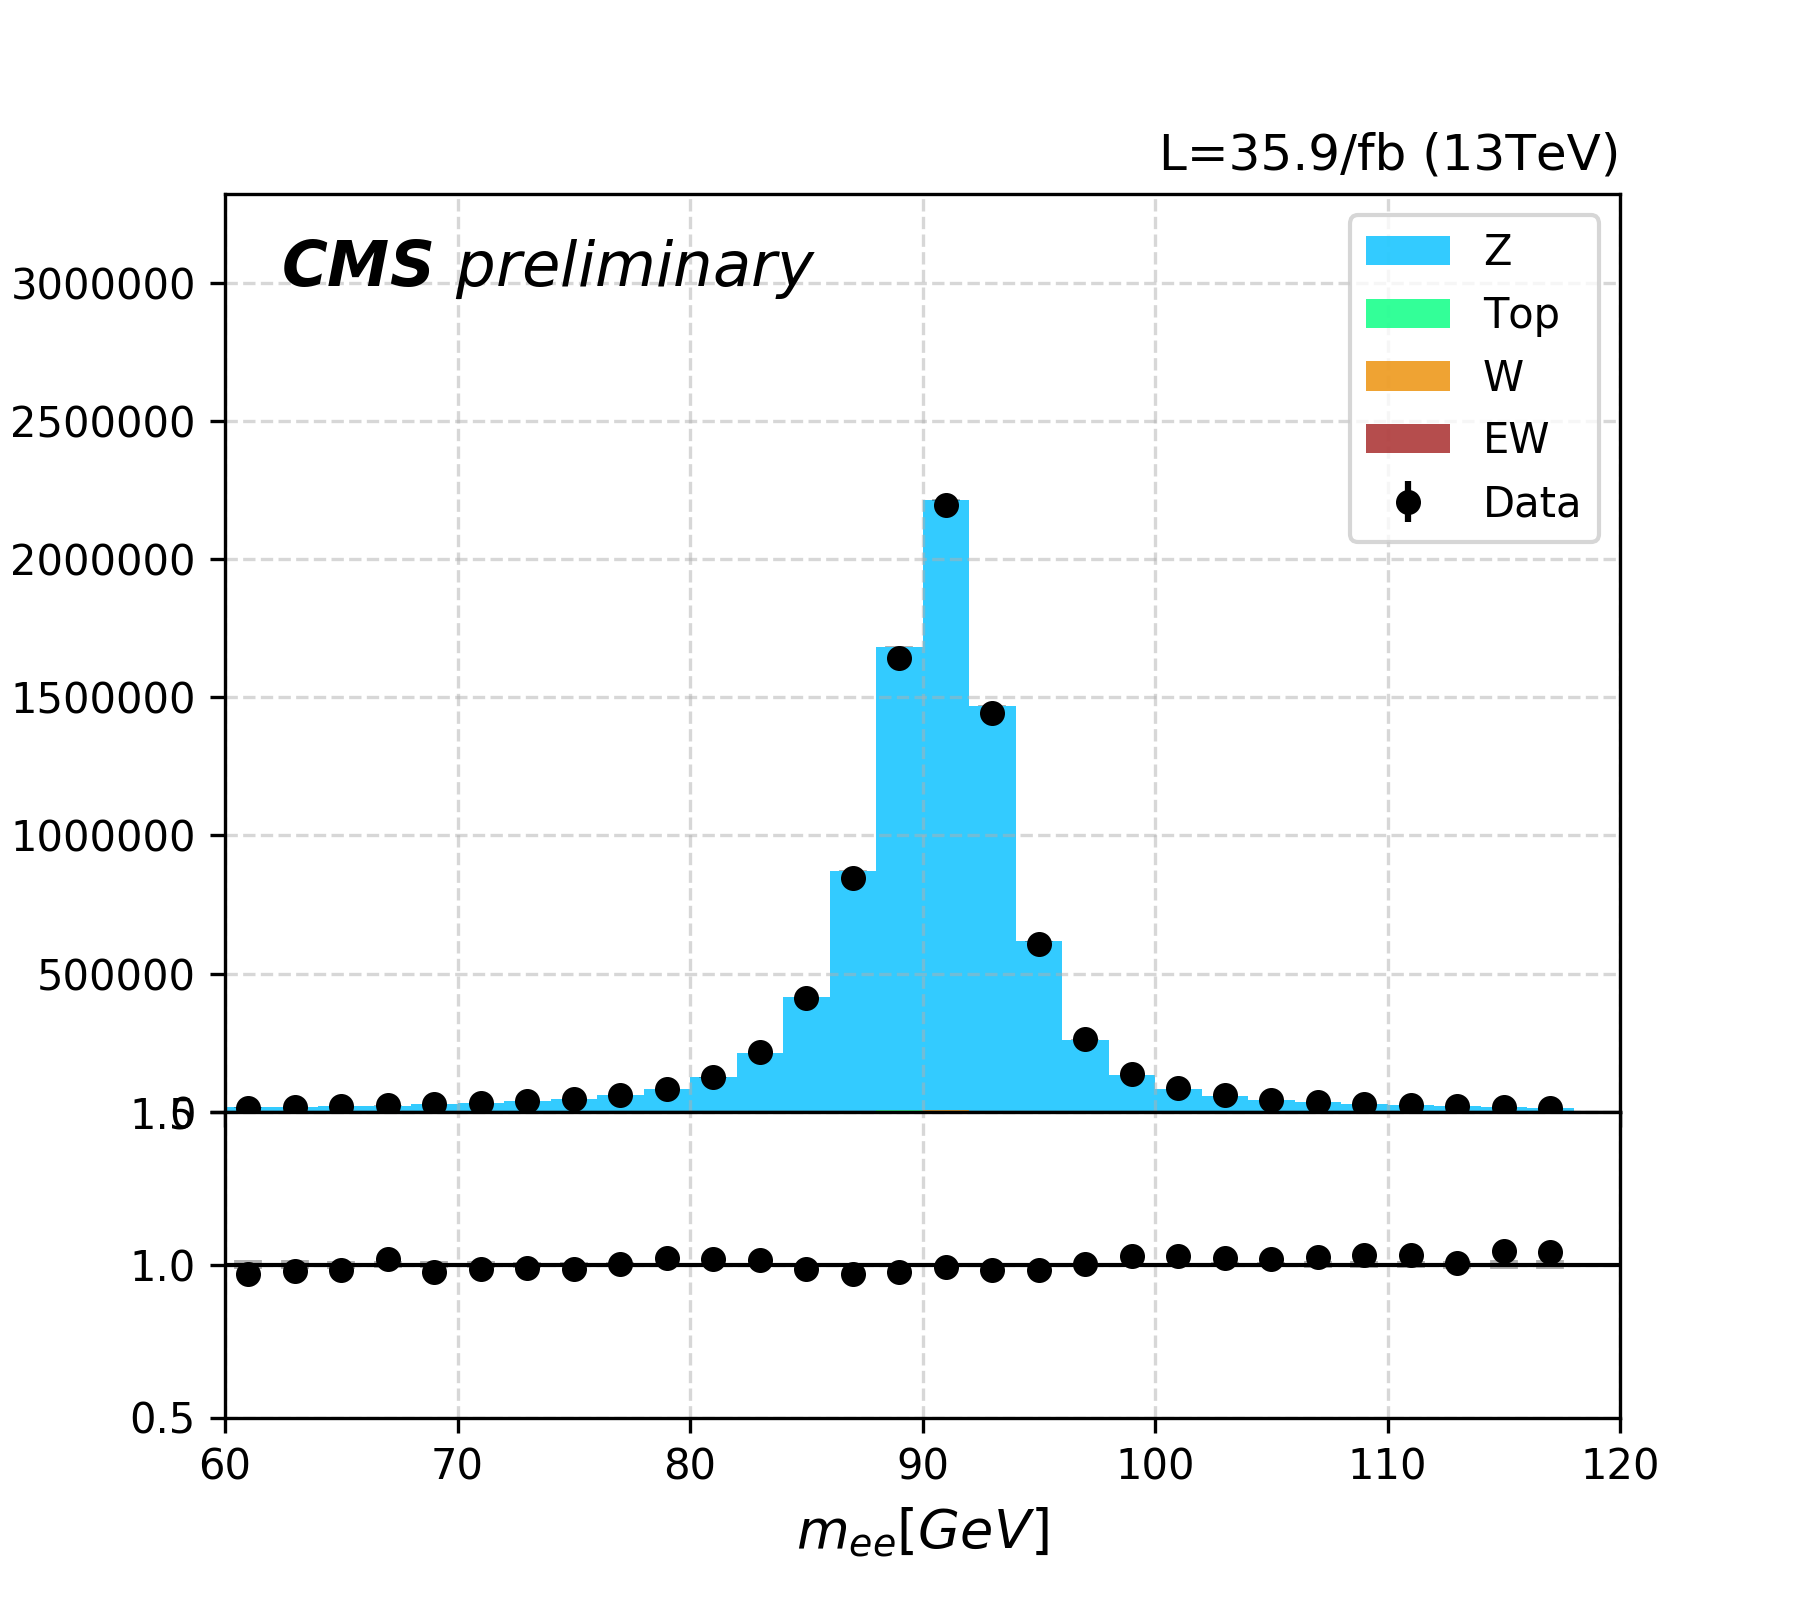
\includegraphics[width=0.6\textwidth]{chapters/Analysis/sectionCalibration/figures/eTrigger/dileptonMass_tag30.png}
    \caption{$m_{ee}$ of the selected events for the measurement of the SF of single-electron trigger efficiency.}
    \label{fig:appendix:ele27TriggerSF}
\end{figure}


The dataset used in the measurement is 2016 re-reco \texttt{SingleElectron} dataset with the golden certificate as luminosity mask. The simulations used in the measurement include \texttt{DYJETSToLL\_M-10to50\_amcatnlo}, \texttt{DYJETSToLL\_M-50\_amcatnlo} and \texttt{TT\_powheg}, reweighted to pile-up $\sigma_{mb} = 69.2\pm 2.3$ nb.

The electrons are selected with tight identification and tight particle-flow isolation with $p^T_e>20$ GeV and $|\eta_e|<2.5$. Corrections to the electrons in the simulation includes energy scale-smear, reconstruction and isolation. Among selected electrons, tagged electrons are defined as $p^T_e>30$ GeV and outside gap between barrel and endcap calorimeter $1.444<|\eta_e|<1.56$, and match with \texttt{HLT\_Ele27\_WPTight\_Gsf} triggering objects. Events are selected by requiring exactly 2 opposite electrons with at least 1 tagged electron and $60<m_{ee}<120$ GeV. This event selection yields a sample of events significantly dominated by Drell-Yan process. The distribution of $m_{ee}$ is shown in fig~\ref{fig:appendix:ele27TriggerSF}. The purity of Drell-Yan (DY) are very high in the selected events. Thus a signal-backgound fit is not necessary to get DY yields.





In each event, if one electron is tagged, the other become a prob. Each event provides either one or two tag-prob pairs. A prob is passing if it match with \texttt{HLT\_Ele27\_WPTight\_Gsf} triggering objects. The trigger efficiencies are calculated by the ratio between the number of passing probs over the total probs in $\pt-\eta$ bins, 

\begin{equation}
    \epsilon (\pt, \eta) = \frac{ N_{\rm passing} (\pt, \eta) } {  N_{\rm total} (\pt, \eta) }.
\end{equation}

\noindent The scale factors are derived by taking the ratio between efficiencies in the data over MC,
\begin{equation}
SF (\pt, \eta) = \frac{\epsilon_{\rm{data}} (\pt, \eta) }{\epsilon_{\rm{MC}} (\pt, \eta) }.
\end{equation}



% \subsection{Result of the Scale Factors}

In 2016 B-F, the data efficiency in the endcap decreases because there is a decrease of signal over noise ratio associated to loss of tracking hits caused by problems in the pre-amplifier of the APV chip. In the mid August 2016, this problem of Si-strip in endcap region is fixed by increase the drain speed of the pre-amplifier. Thus the trigger efficiencies are improved in 2016 GH. So the measurement of the scale factor of the trigger efficiency is divided into to two parts based on data taking periods, the 2016 B-F and 2016 GH.


The 2D maps of $\epsilon_{\rm{data}}$, $\epsilon_{\rm{MC}}$ and $SF$ in both 2016 B-F and 2016 GH are shown in Figure~\ref{fig:appendix:ele27SF}. Figure~\ref{fig:appendix:ele27SFperiods} shows the $SF$ in each 2016 data taking period, where the improvement in the G period is clear.



\begin{figure}
    \centering
    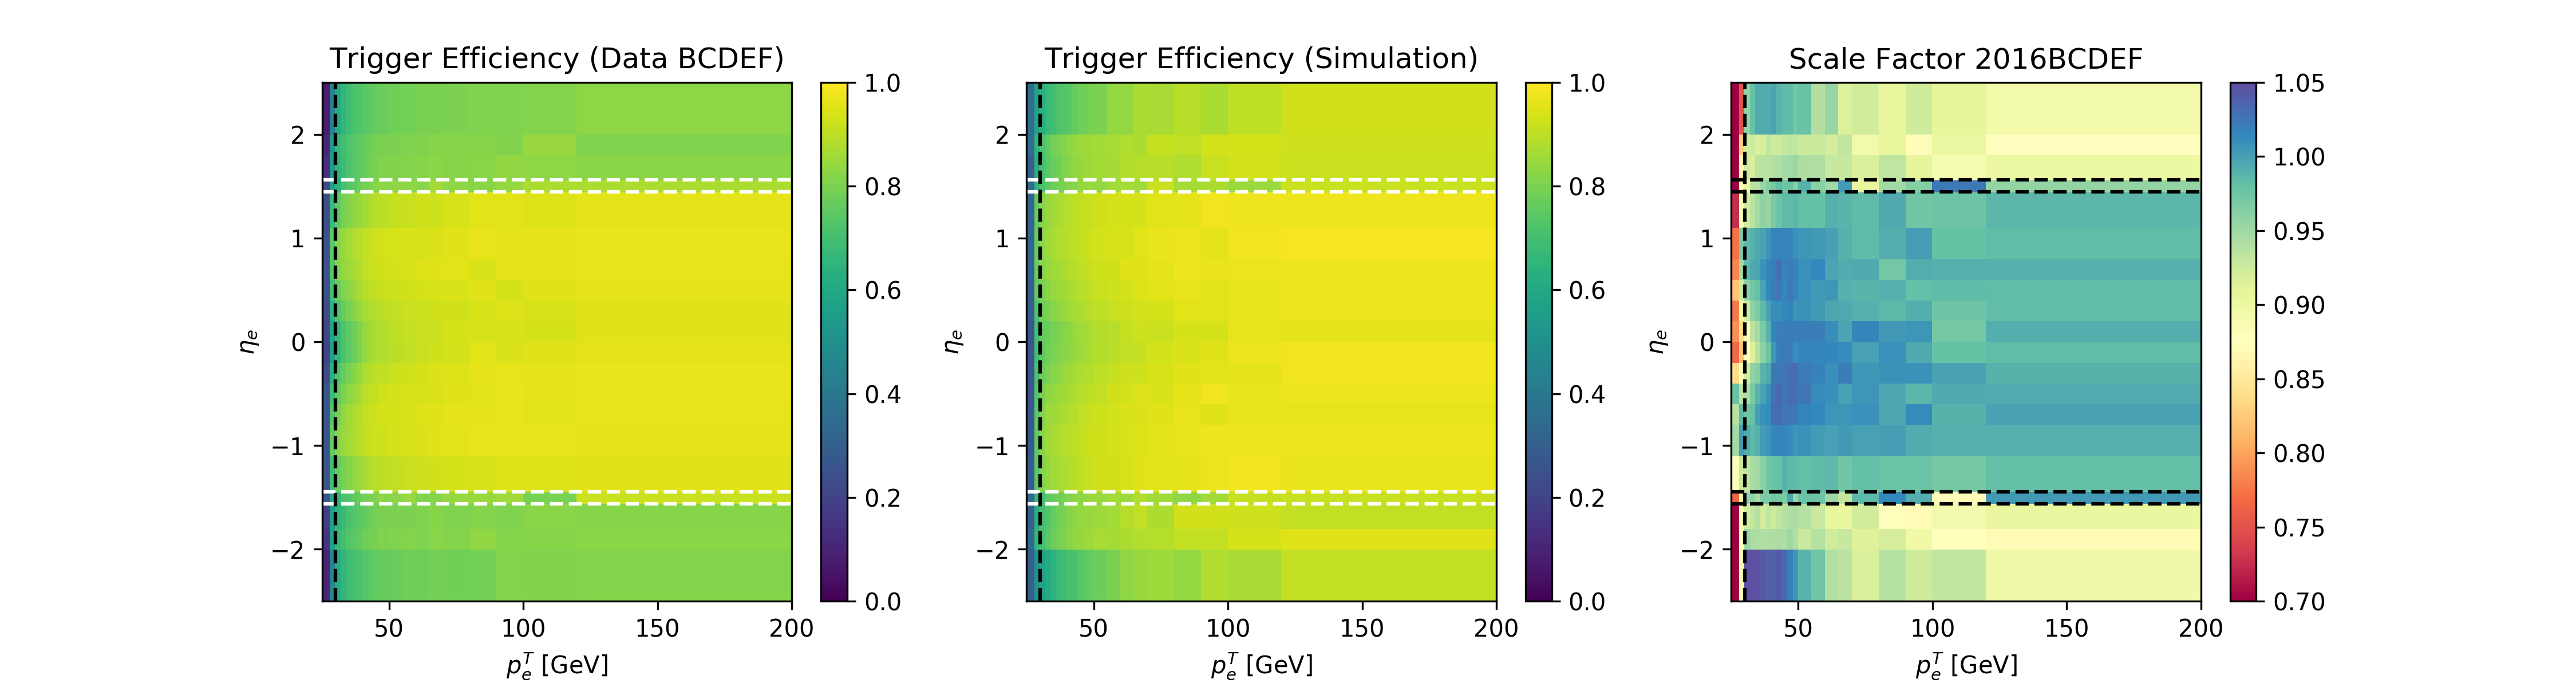
\includegraphics[width=0.99\textwidth]{chapters/Analysis/sectionCalibration/figures/eTrigger/eff2d_BCDEF.png}
    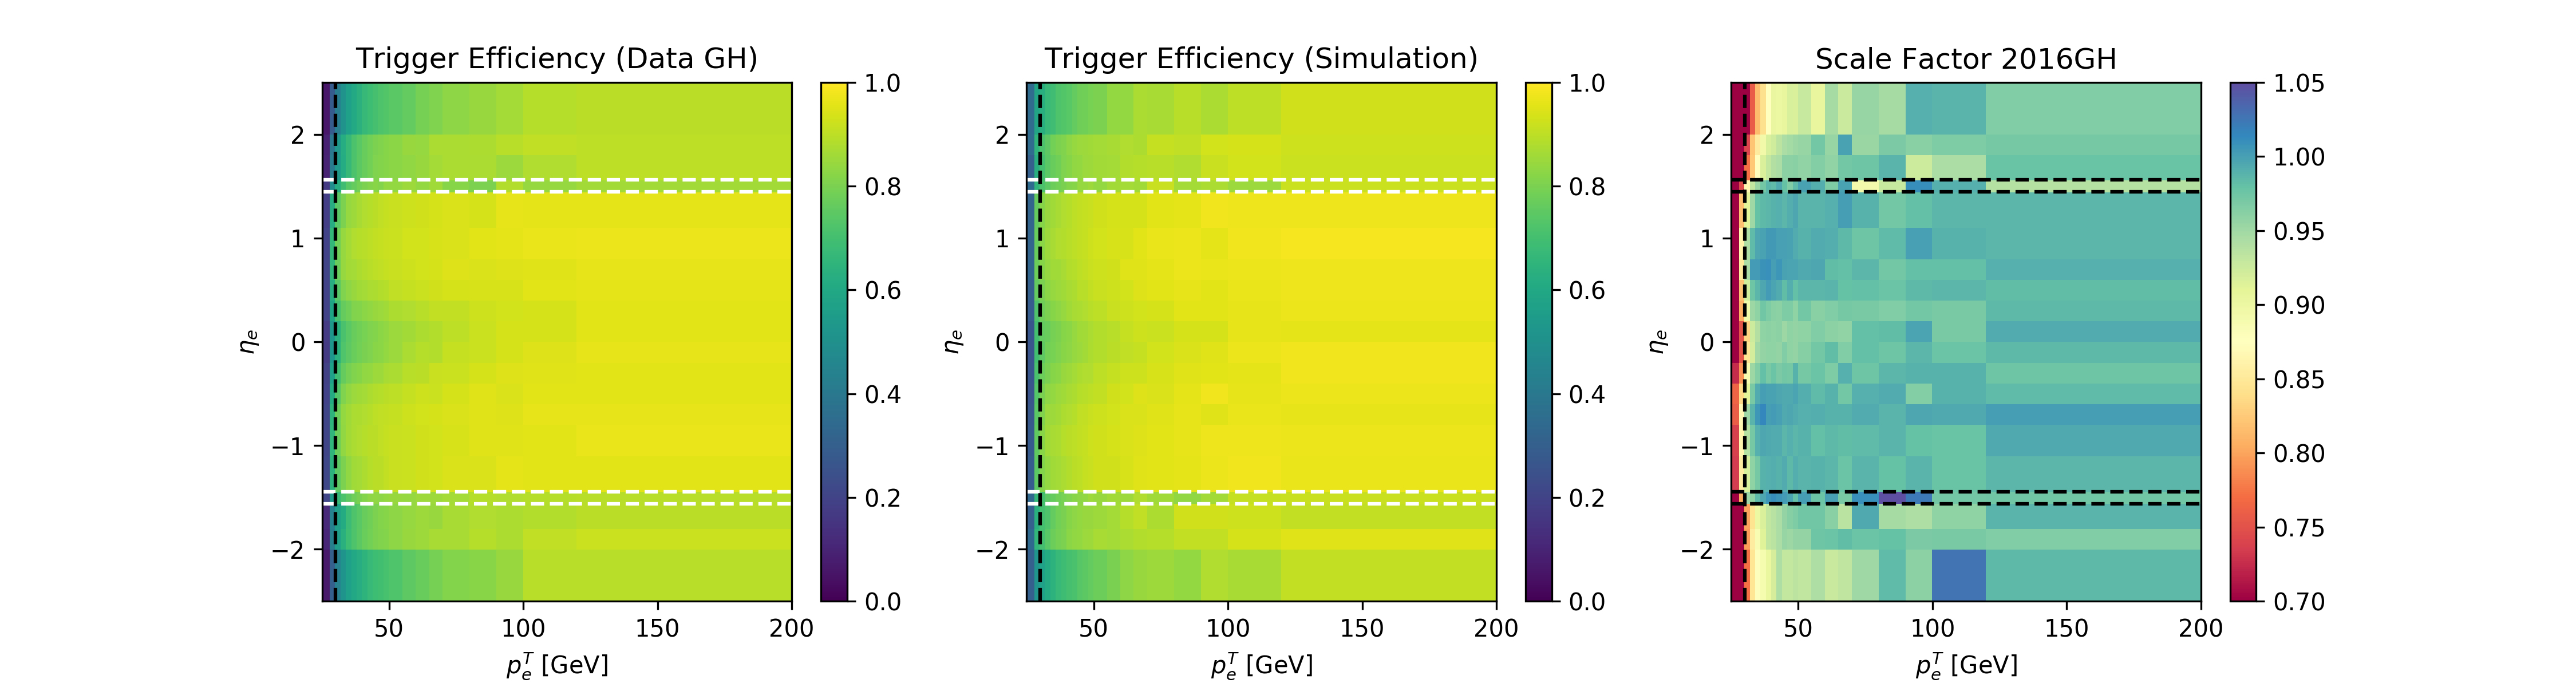
\includegraphics[width=0.99\textwidth]{chapters/Analysis/sectionCalibration/figures/eTrigger/eff2d_GH.png}
    \caption{The 2D maps of $\epsilon_{\rm{data}}$, $\epsilon_{\rm{MC}}$ and $SF$ in both 2016 B-F and 2016 GH.}
    \label{fig:appendix:ele27SF}
\end{figure}



\begin{figure}
    \centering
    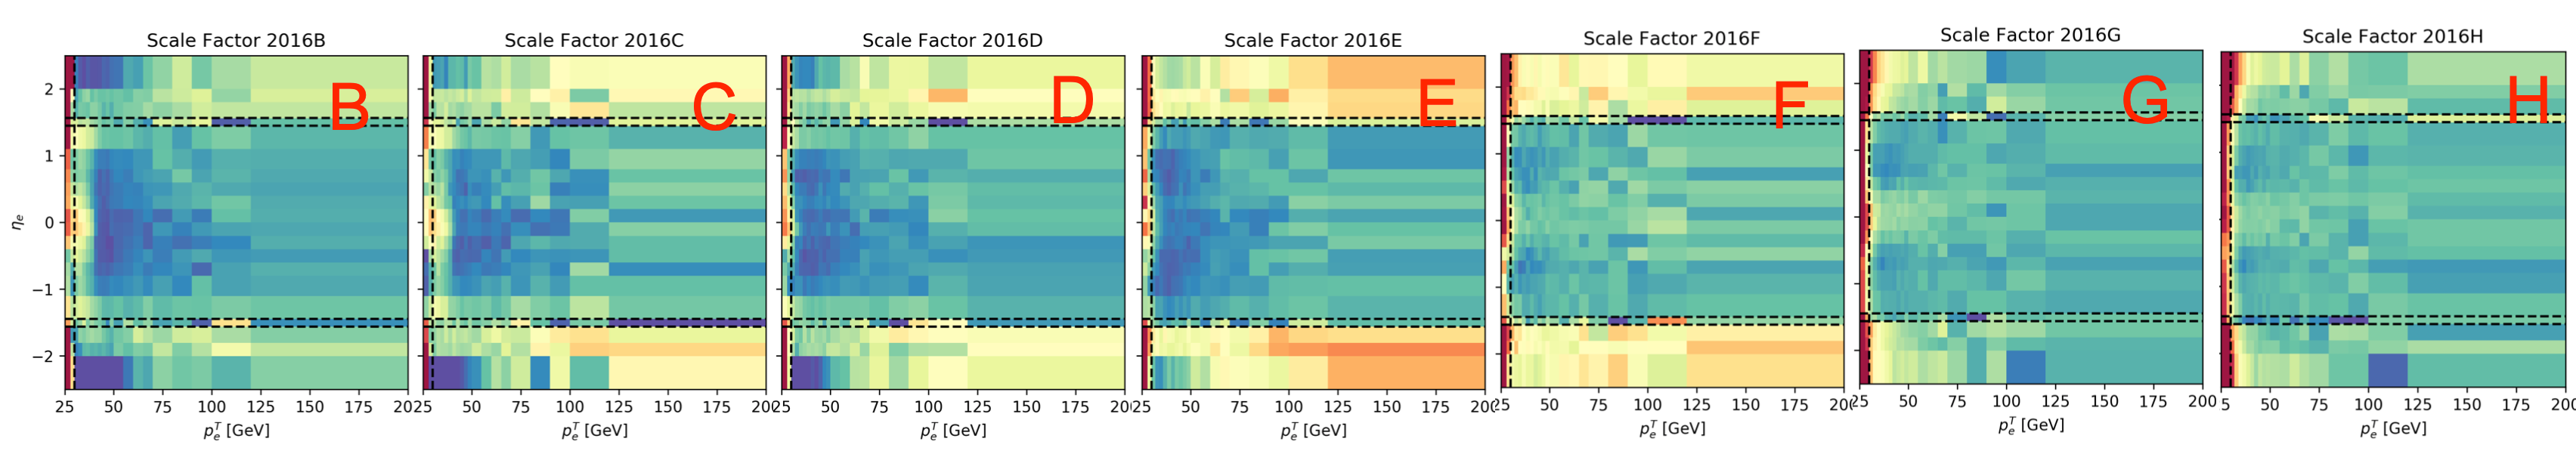
\includegraphics[width=0.99\textwidth]{chapters/Analysis/sectionCalibration/figures/eTrigger/result_period.png}
    \caption{$SF$ in each 2016 data taking period.}
    \label{fig:appendix:ele27SFperiods}
\end{figure}





For the two parts, 2016 B-F and GH, the systematical uncertainties are estimated by the "two shifts" approach described above. The total uncertainty combines the statistical and systematical uncertainties from tag and prob "two shifts". The final result of the SF and the associated uncertainties are shown in fig~\ref{fig:eTrSF_err_BCDEF} and \ref{fig:eTrSF_err_GH}.

\begin{figure}
    \centering
    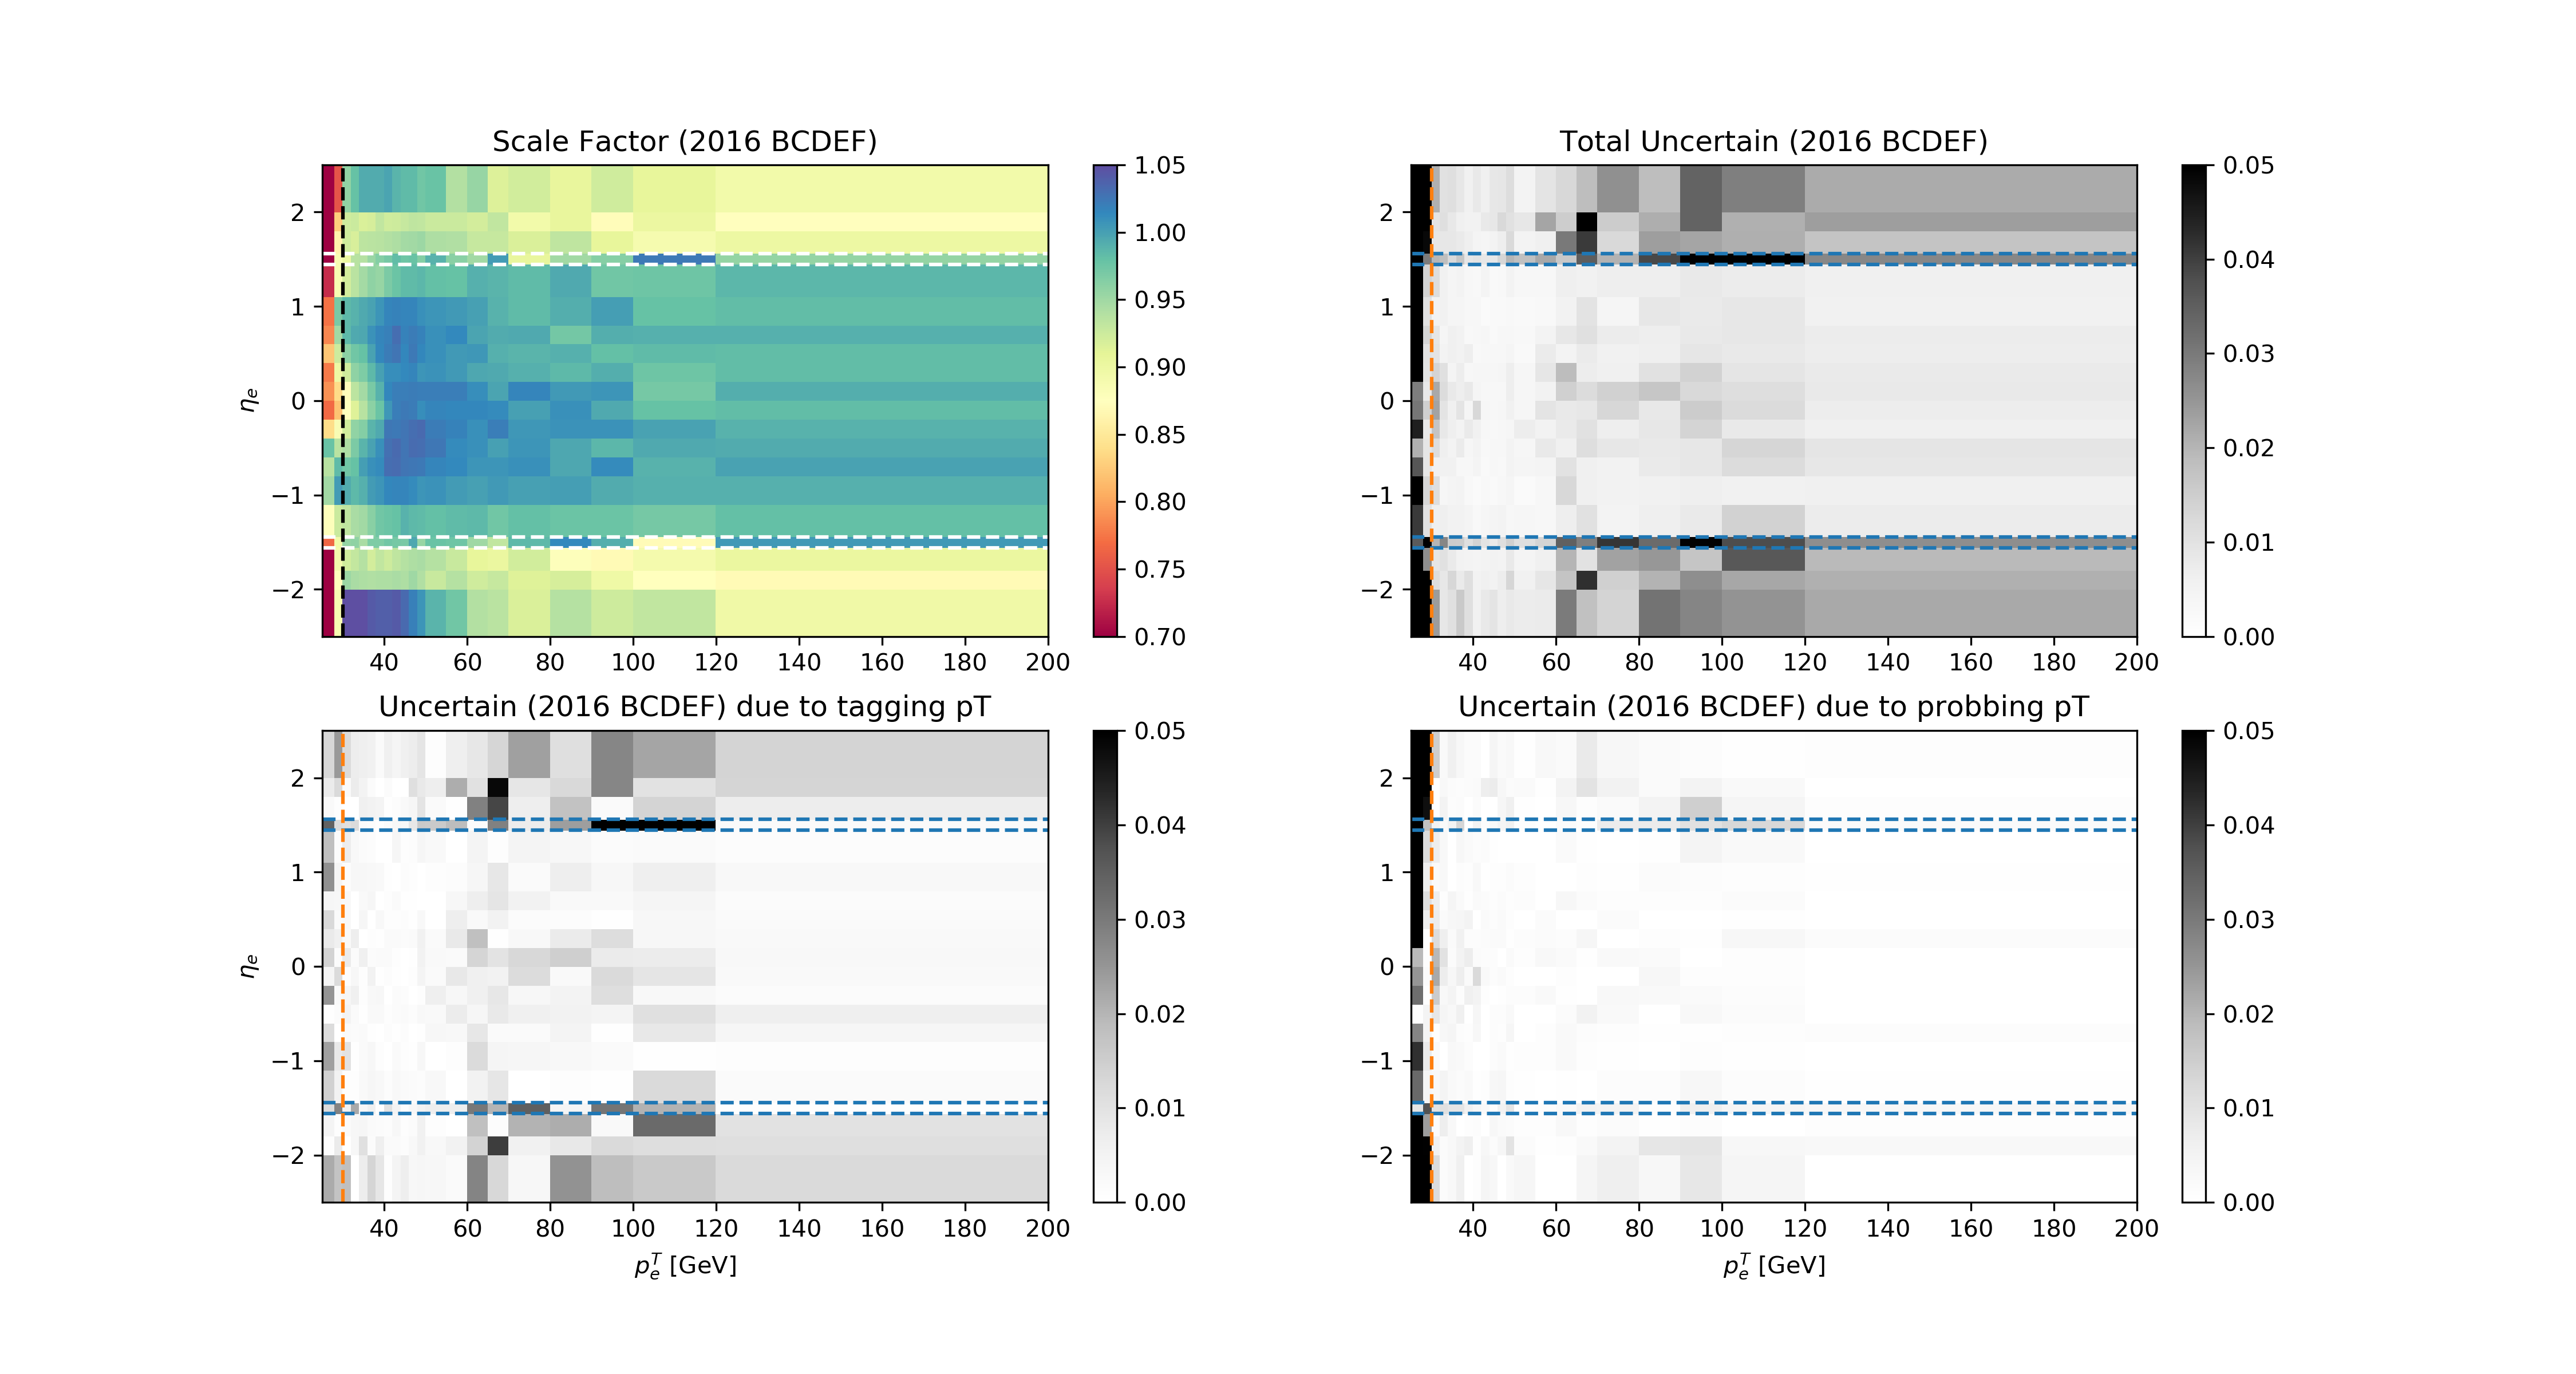
\includegraphics[width=0.99\textwidth]{chapters/Analysis/sectionCalibration/figures/eTrigger/result_BCDEF.png}
    \caption{SF and the associated uncertainties in the 2016 B-F.}
    \label{fig:eTrSF_err_BCDEF}
\end{figure}

\begin{figure}
    \centering
    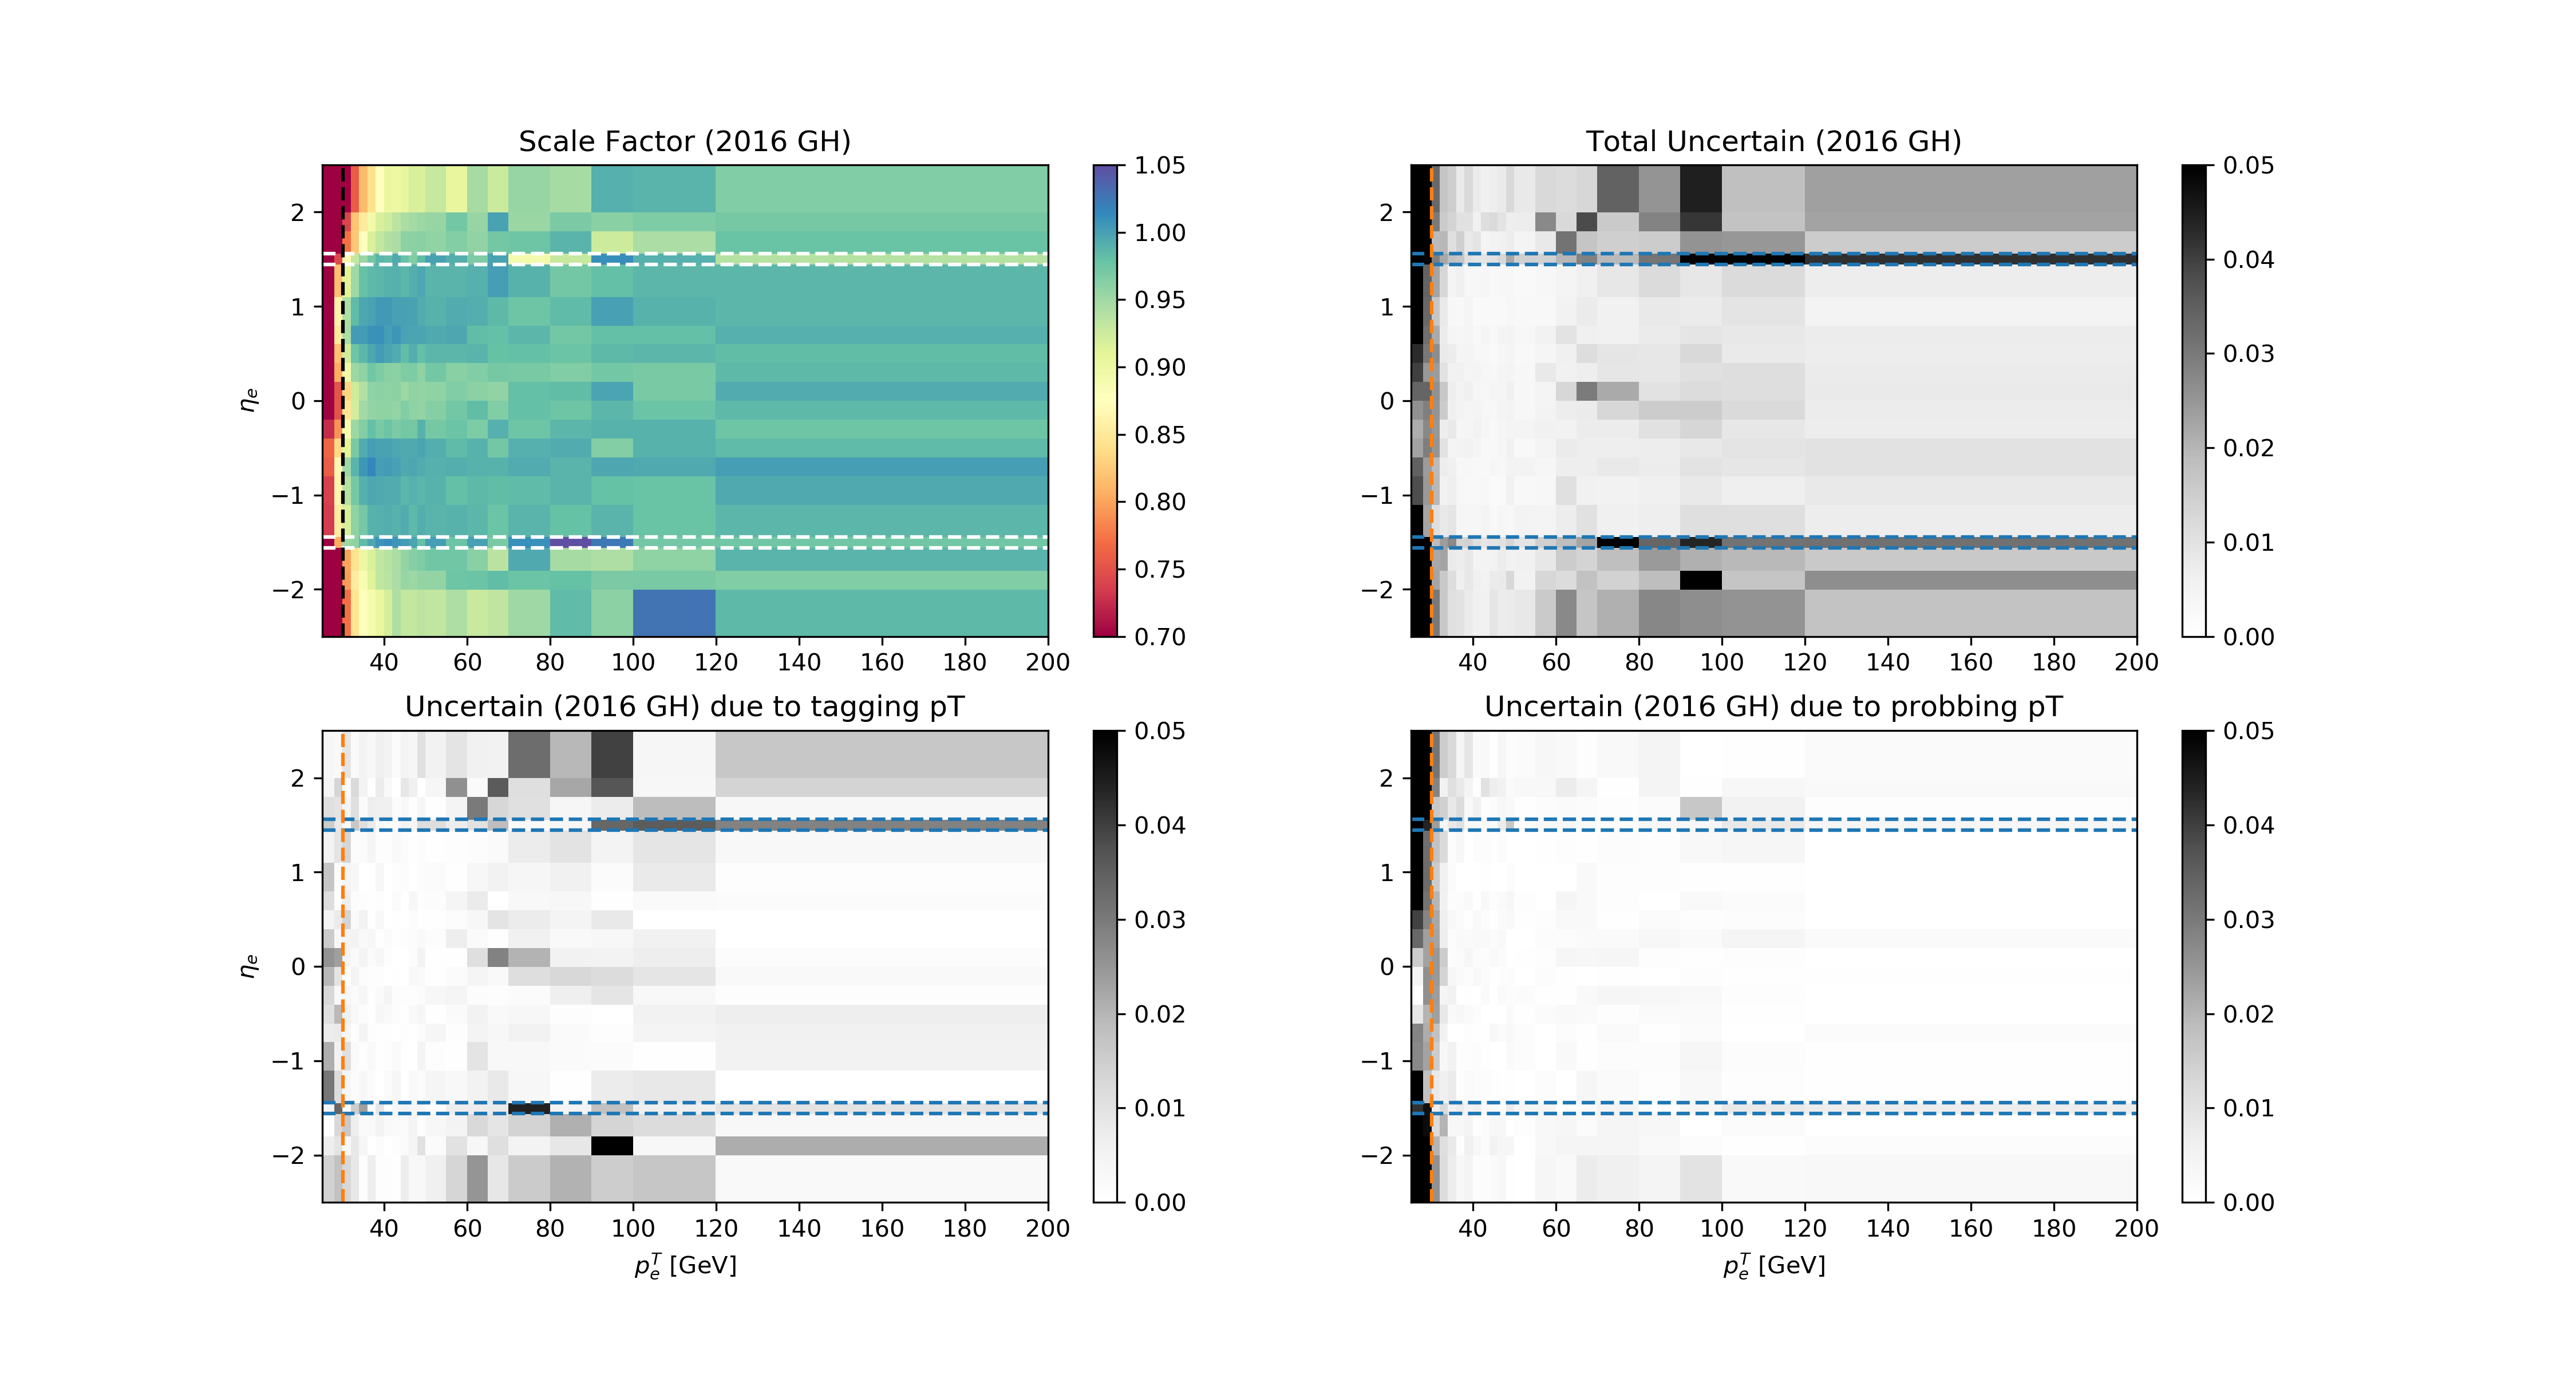
\includegraphics[width=0.99\textwidth]{chapters/Analysis/sectionCalibration/figures/eTrigger/result_GH.png}
    \caption{SF and the associated uncertainties in the 2016 GH.}
    \label{fig:eTrSF_err_GH}
\end{figure}

\FloatBarrier




\subsection{Measurement of Scale Factors for Jet Faking Hadronic Tau}
\label{sec:analysis:calibration:jetToTauh}


% \subsection{Measurement Approach}
In both the signal region and control region, $\mu \tau$ and $e \tau$ final states have sizable contributions from electron or muon plus a jet misidentified as a hadronic tau.  For correction to tau identification efficiency, tau POG has provided $SF (\tau_h \to \tau_h)$ measured with tag-prob technique at different identification working points.  However, regarding the $SF (j \to \tau_h)$, because the jet environment varies from analysis to analysis, tau POG suggests to measure it ourselves in a side-band region to correct $j \to \tau_h$ contributions and access corresponding uncertainties.

Our measurement of $SF (j\to \tau_h)$ is based on two regions, $t\bar{t}$ region which is enriched with b-jets identified as hadronic taus, $Z+jets$ region which is enriched with light jets identified as hadronic taus. Both Tight and VTight $\tau_h$ identification working points are considered.

\begin{itemize}
    \item $t\bar{t}$ region: $e\mu+\tau_h$ final state is selected. The selection requires exactly one muon and one electron with tight identification and isolation, plus one hadronic tau passing Tight or VTight working point. Corrections to reconstruction and selection of electron and muon are applied. The events has to fire either single muon trigger or single electron trigger.  The \pt threshold for triggering muon (electron) is 25 (30) GeV, while for non-triggering muon (electron) is 10 (20) GeV.  This selects a sample enriched with $t\bar{t}$ with $b \to \tau_h$. The kinematics of $e\mu+\tau$ final state events are shown in Figure~\ref{fig:appendix:fakeTauId:emutau}.
    
    
    \item $Z+jets$ region: $\mu\mu+\tau_h$ and $ee+\tau_h$ final state are selected.  The selection requires exactly two muons or two electrons with tight identification and isolation, plus one hadronic tau passing Tight or VTight working point.  Corrections to reconstruction and selection of electron and muon are applied. The trigger and \pt thresholds of leptons are the same as $e\mu+\tau_h$ final state.  This selects a sample enriched with $Z + jet$ with a light jet misidentified as $\tau_h$. The kinematics of $\mu\mu+\tau$ and $ee+\tau$ final states are shown in Figure~\ref{fig:appendix:fakeTauId:mumutau} and \ref{fig:appendix:fakeTauId:eetau}.
\end{itemize}

\noindent Note that the selections of $e\mu+\tau$, $\mu\mu+\tau$, $ee+\tau$ are developed based on the $e\mu$, $\mu\mu$, $ee$ selection in the main Br analysis,
using the same dilepton selection but requiring one additional Tight or VTight $\tau_h$. The origins of selected $\tau_h$ are tagged based on MC truth.  For each selected $\tau_h$, if there is a gen-level $\tau_h$ found within $\delta R = 0.3$, the $\tau_h$ is tagged as true identification.  If not a true identification, we try to match it with jet in the vetoed-jet collection and tag it as $j \to \tau_h$, flavor of which equals to the MC flavor of the jet correspondence.  In the rare cases where multiple jet correspondences are found, the one with highest pT is considered.  If neither gen-level $\tau_h$ match nor jet correspondence are found, the $\tau_h$ is untagged, which mainly due to $e \to \tau_h$. The gen-level  origin of $\tau_h$ are included in Figure~\ref{fig:appendix:fakeTauId:emutau,fig:appendix:fakeTauId:mumutau,fig:appendix:fakeTauId:eetau}.


\begin{figure}
    \centering
    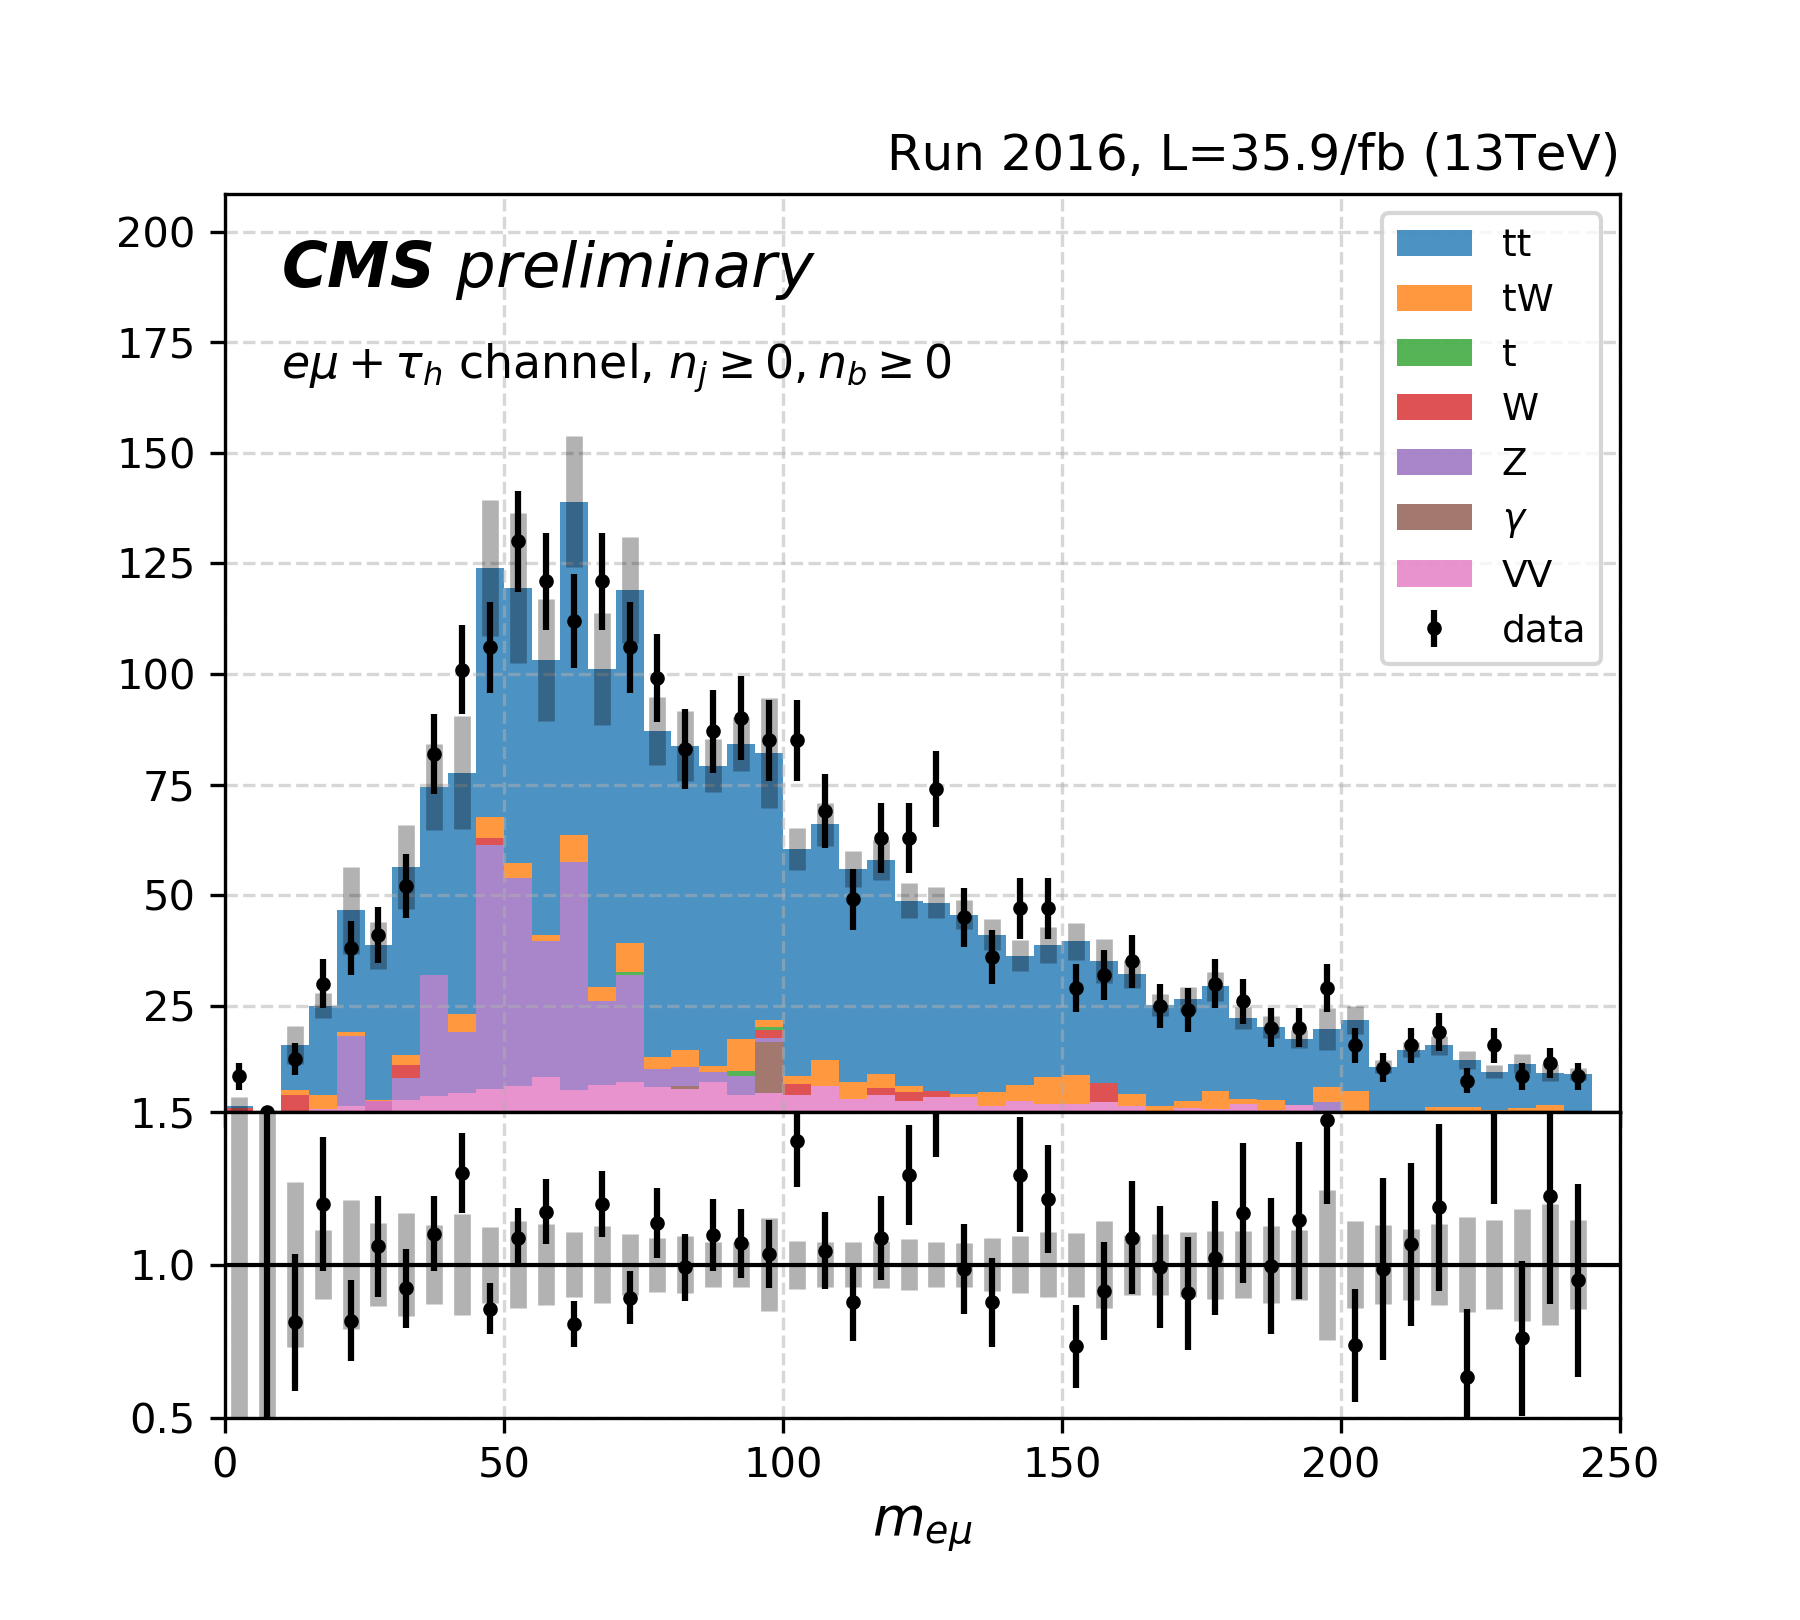
\includegraphics[width=0.4\textwidth]{chapters/Analysis/sectionCalibration/figures/jetToTauh/emutau_dilepton_mass_pickles_lltauTight.png}
    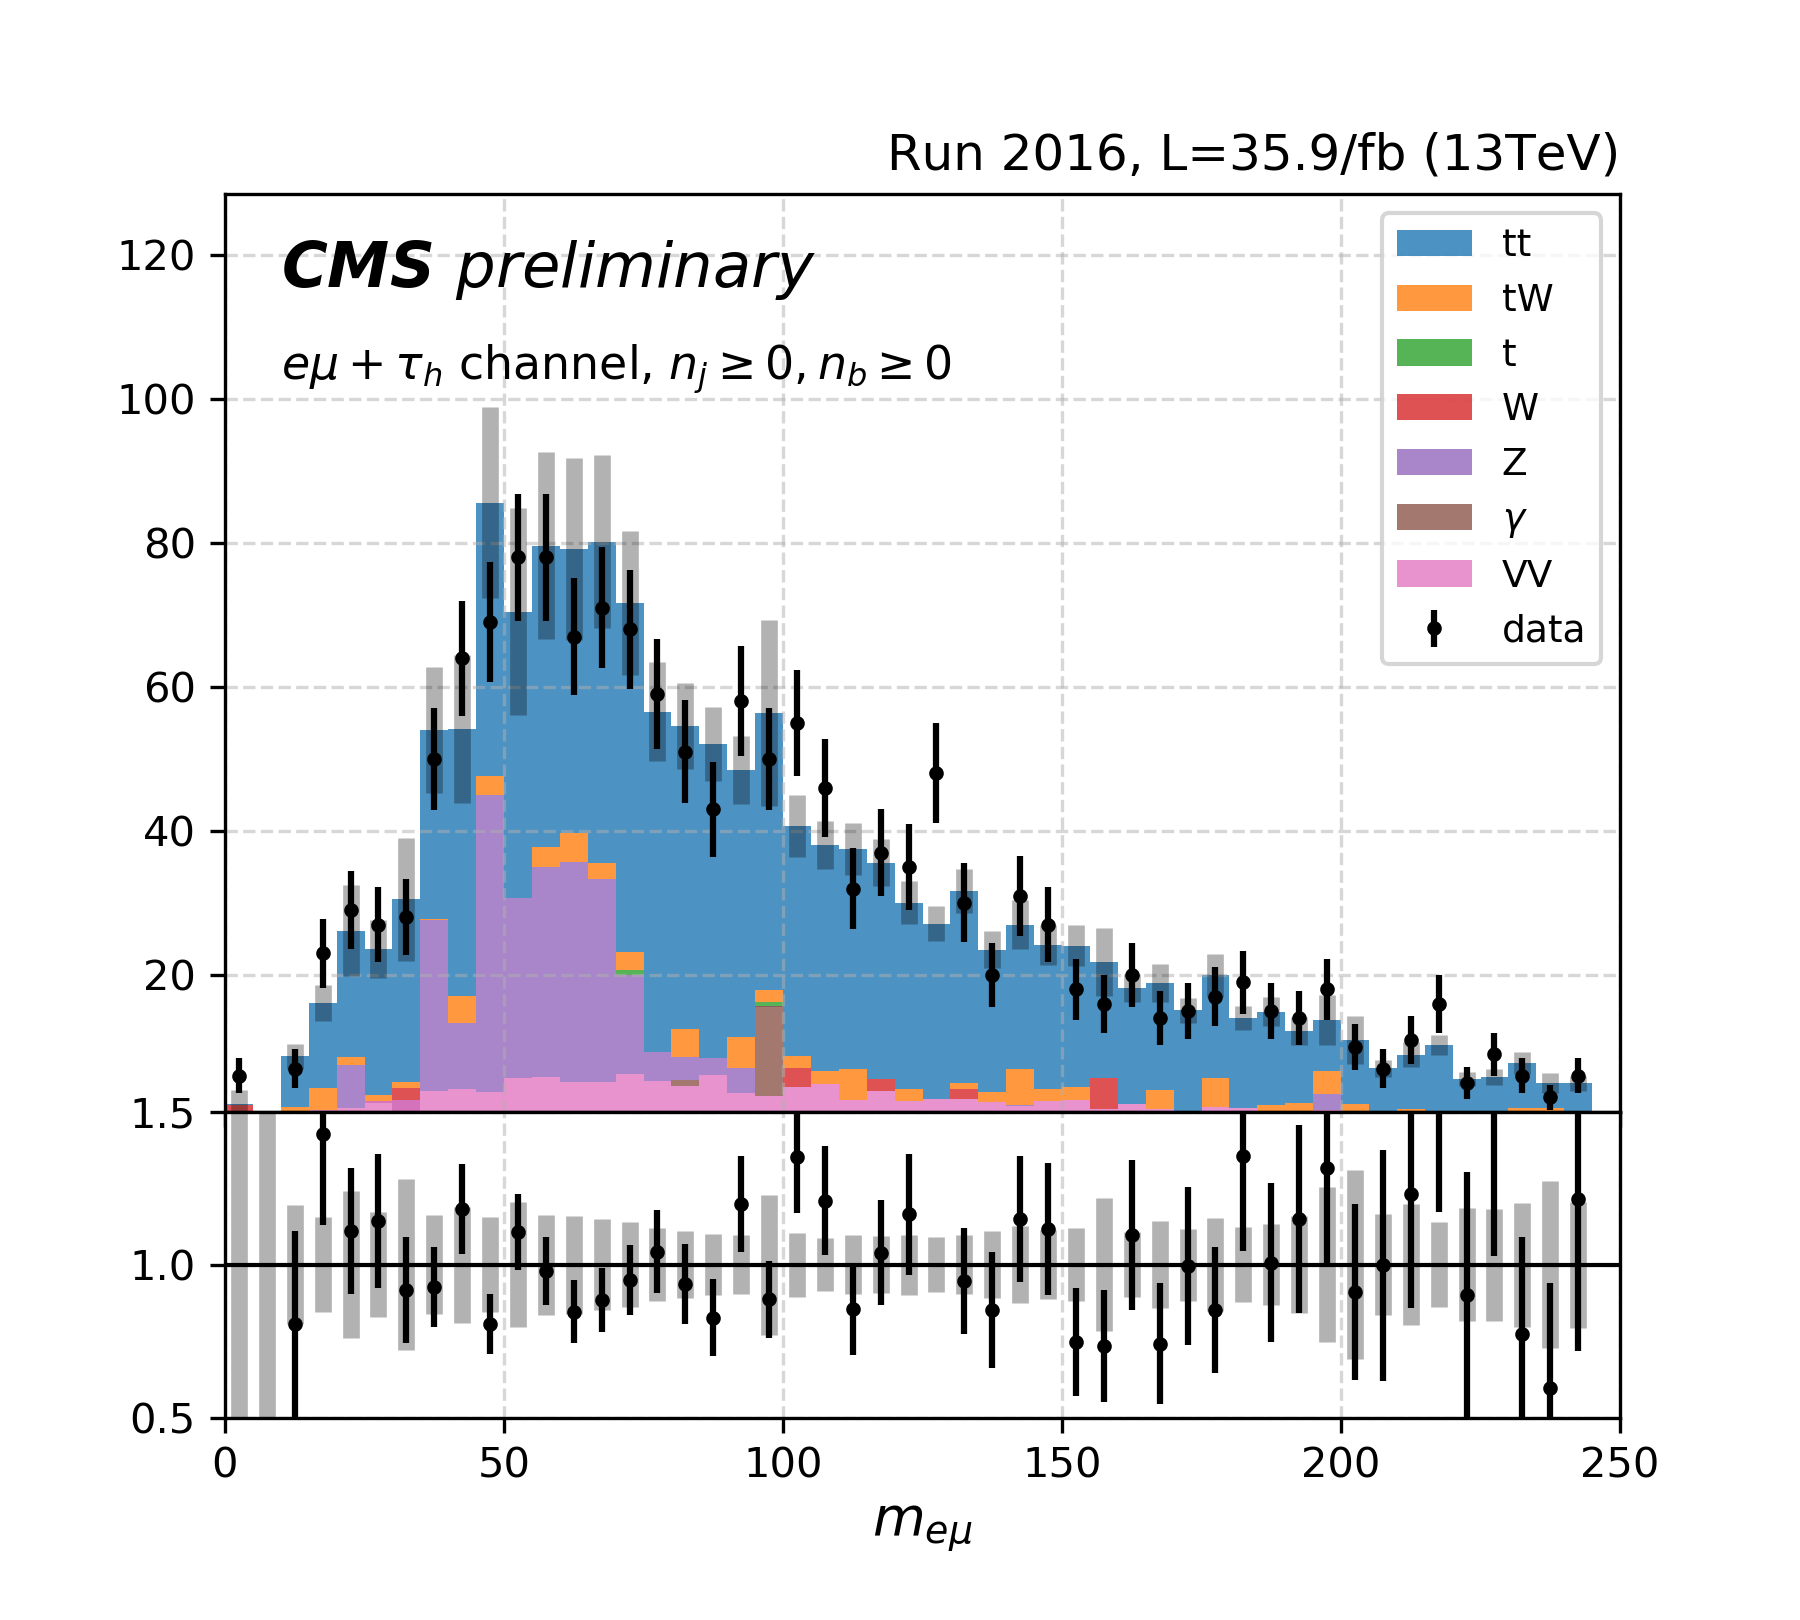
\includegraphics[width=0.4\textwidth]{chapters/Analysis/sectionCalibration/figures/jetToTauh/emutau_dilepton_mass_pickles_lltauVTight.png}
    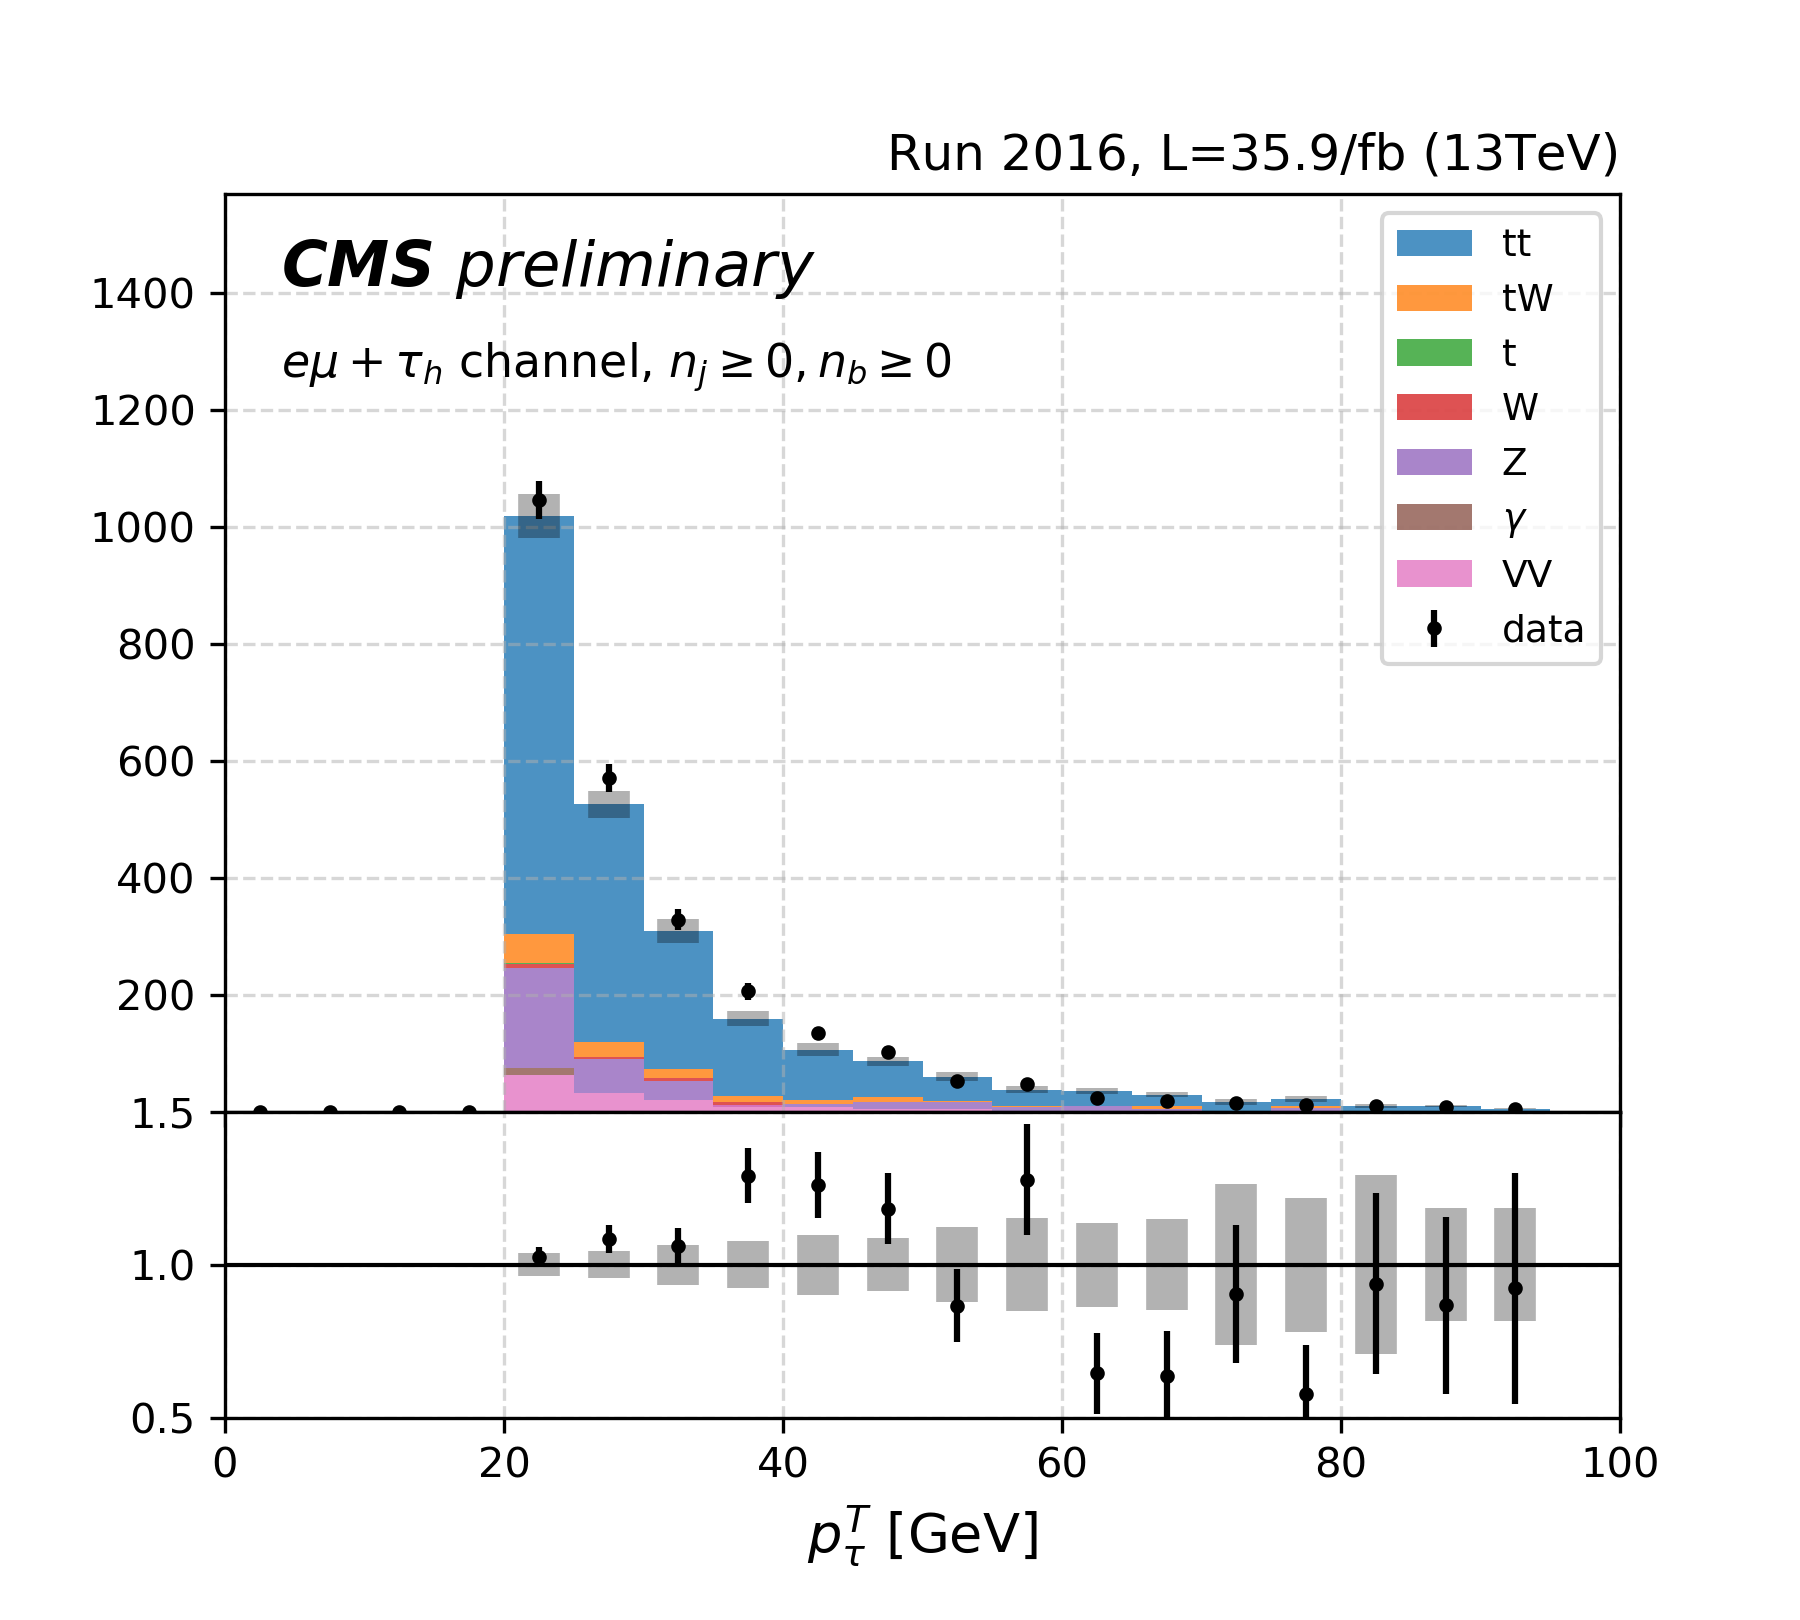
\includegraphics[width=0.4\textwidth]{chapters/Analysis/sectionCalibration/figures/jetToTauh/emutau_tauPt_pickles_lltauTight.png}
    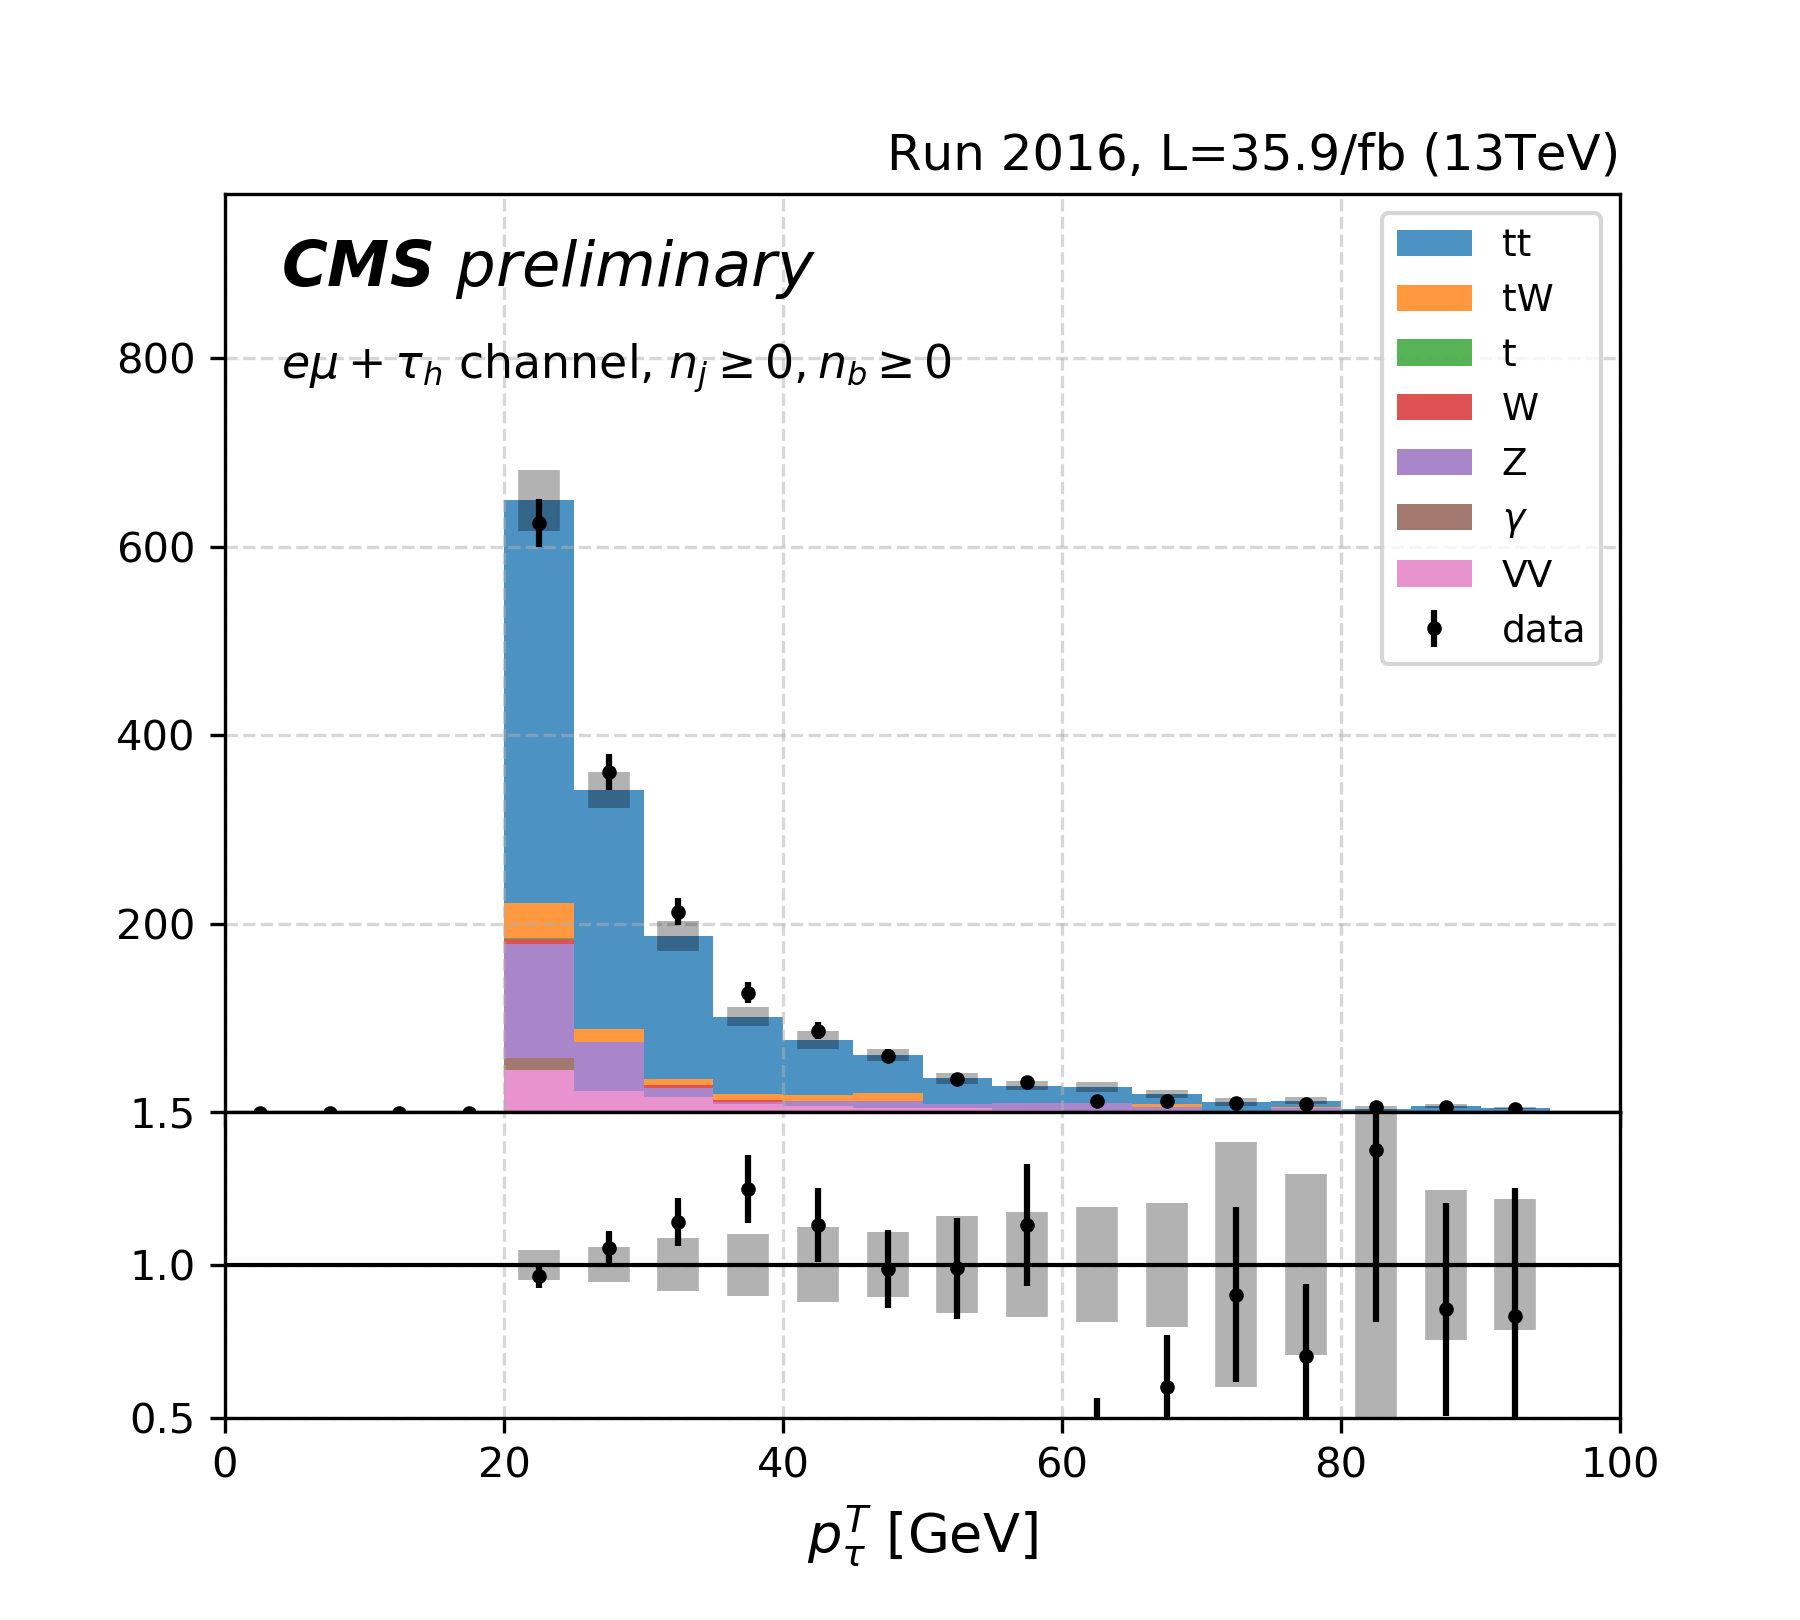
\includegraphics[width=0.4\textwidth]{chapters/Analysis/sectionCalibration/figures/jetToTauh/emutau_tauPt_pickles_lltauVTight.png}
    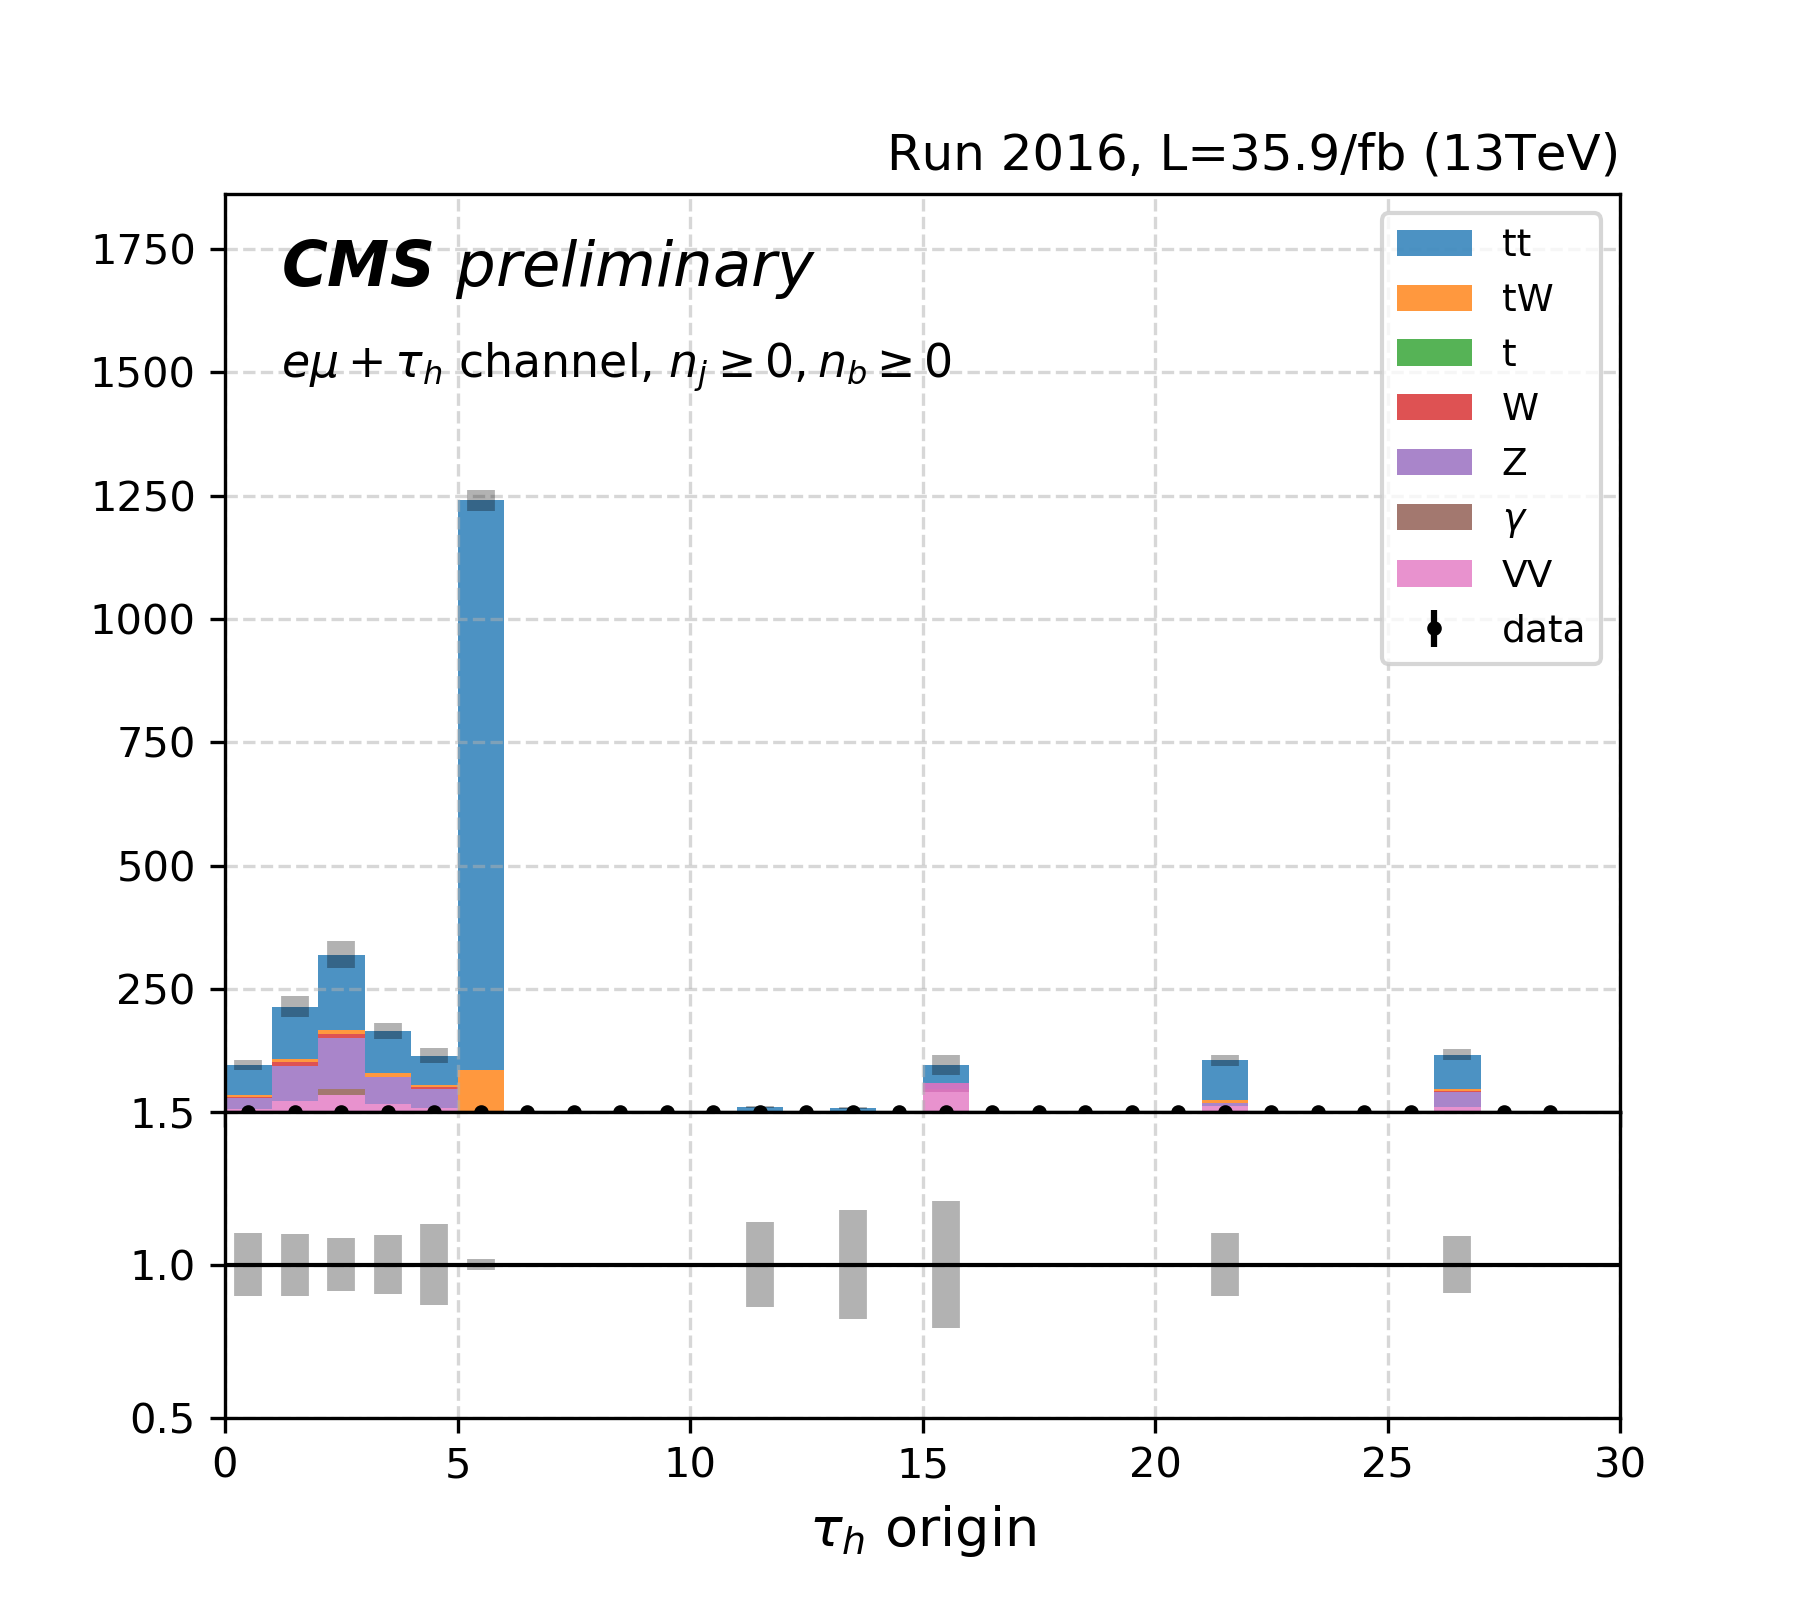
\includegraphics[width=0.4\textwidth]{chapters/Analysis/sectionCalibration/figures/jetToTauh/emutau_tauGenFlavor_pickles_lltauTight.png}
    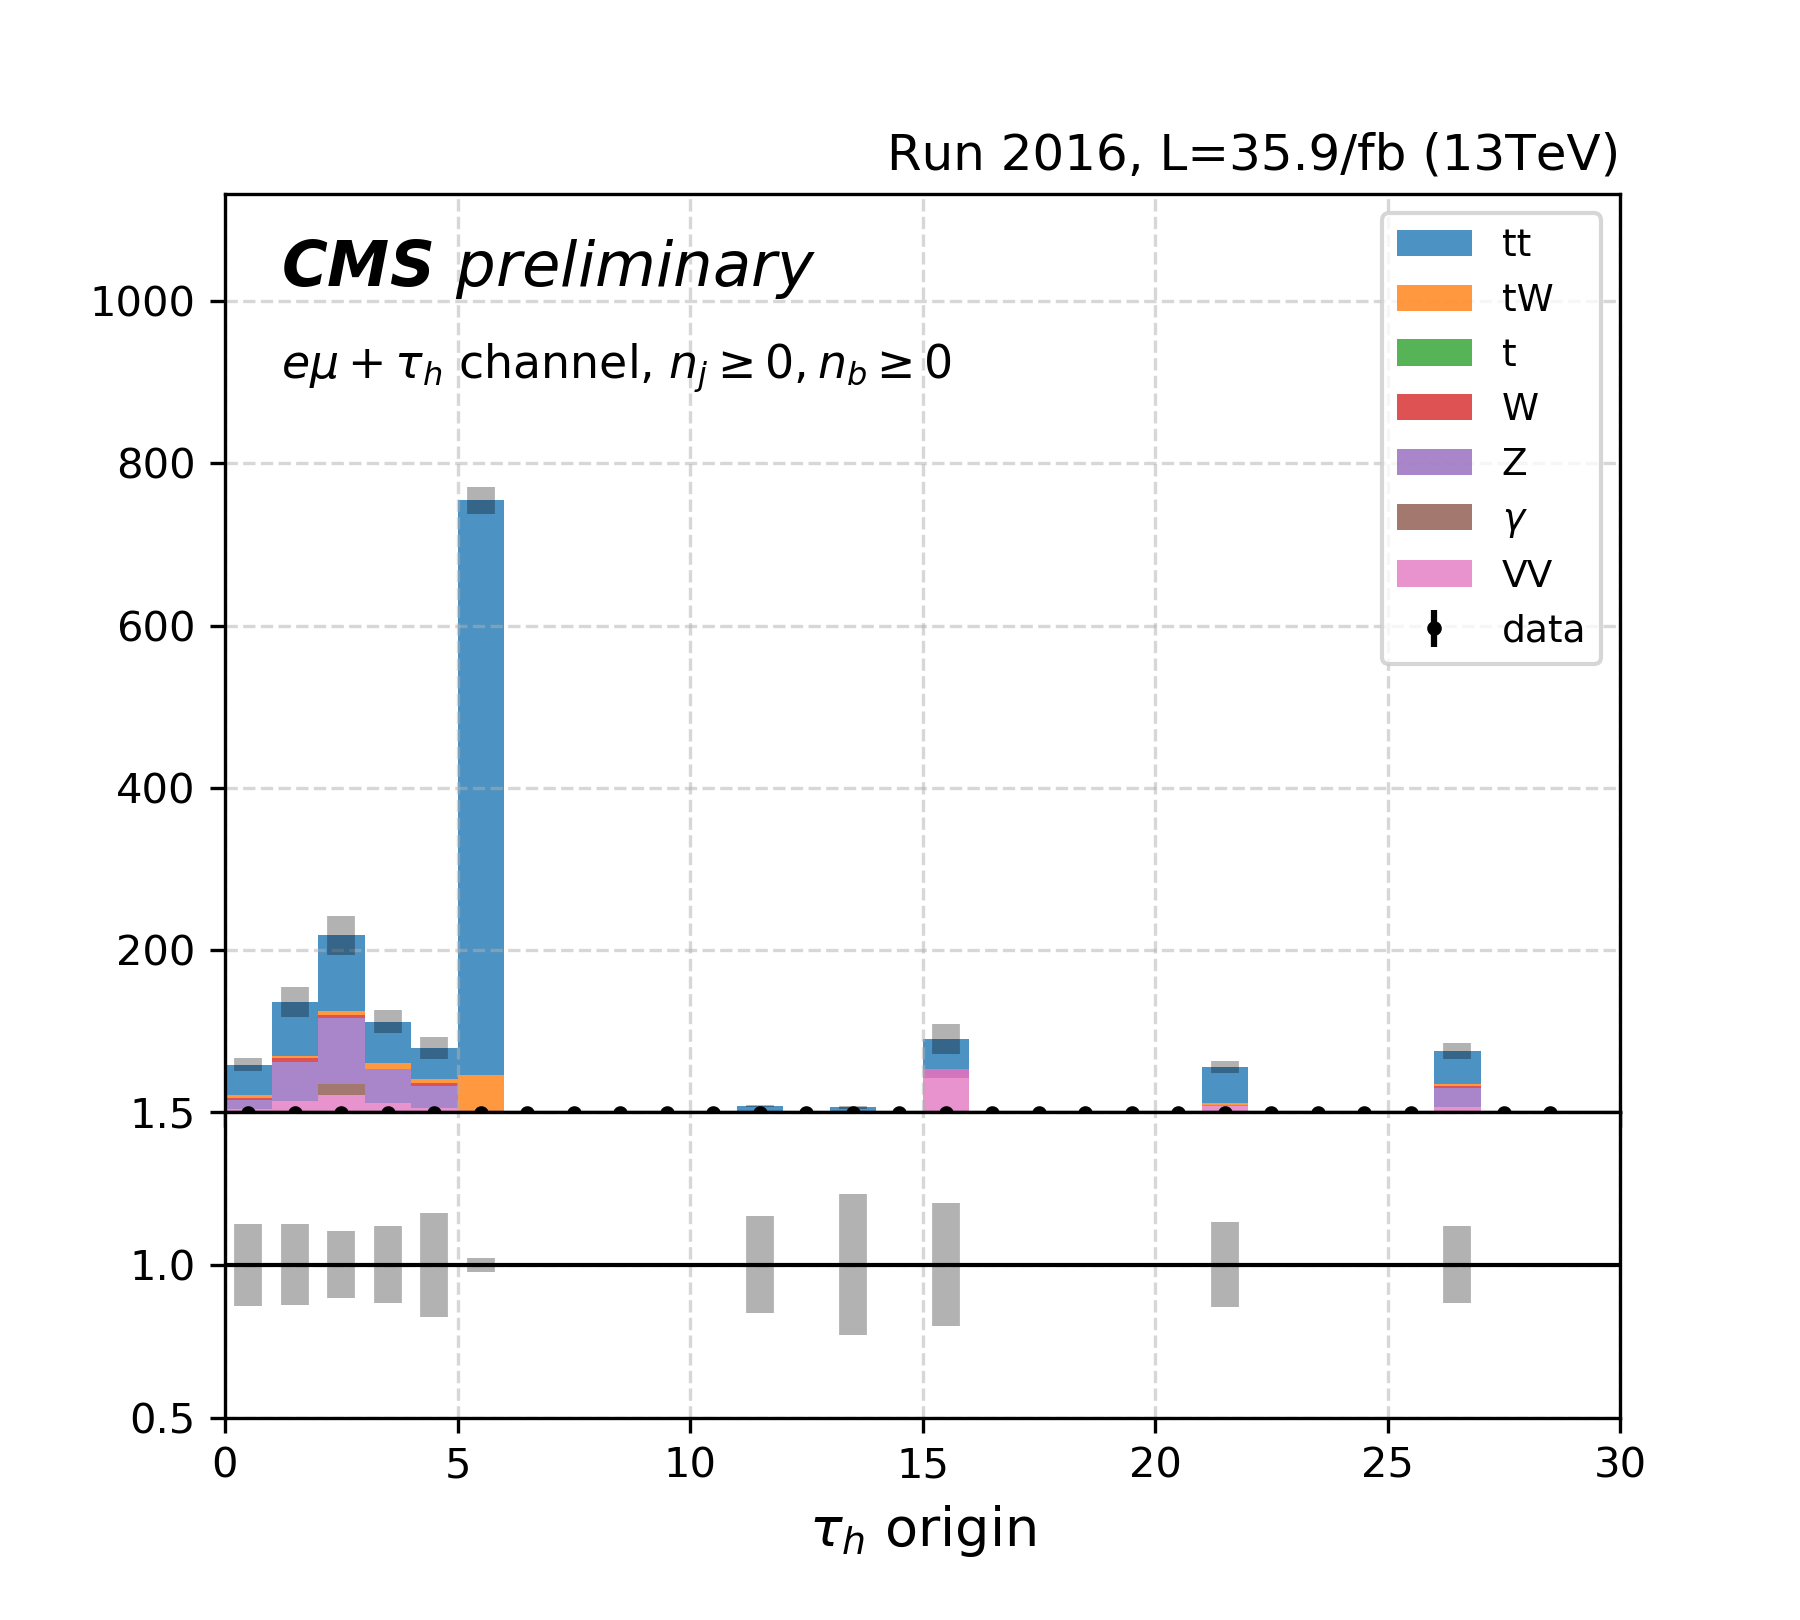
\includegraphics[width=0.4\textwidth]{chapters/Analysis/sectionCalibration/figures/jetToTauh/emutau_tauGenFlavor_pickles_lltauVTight.png}
    \caption{Distributions of $m_{e\mu}$, $\tau_h$ \pt and gen-level $\tau_h$ origin in the $e\mu+\tau$ channel. The left and right column shows the Tight and VTight $\tau_h$ WP respectively.}
    \label{fig:appendix:fakeTauId:emutau}
\end{figure}

\begin{figure}
    \centering
    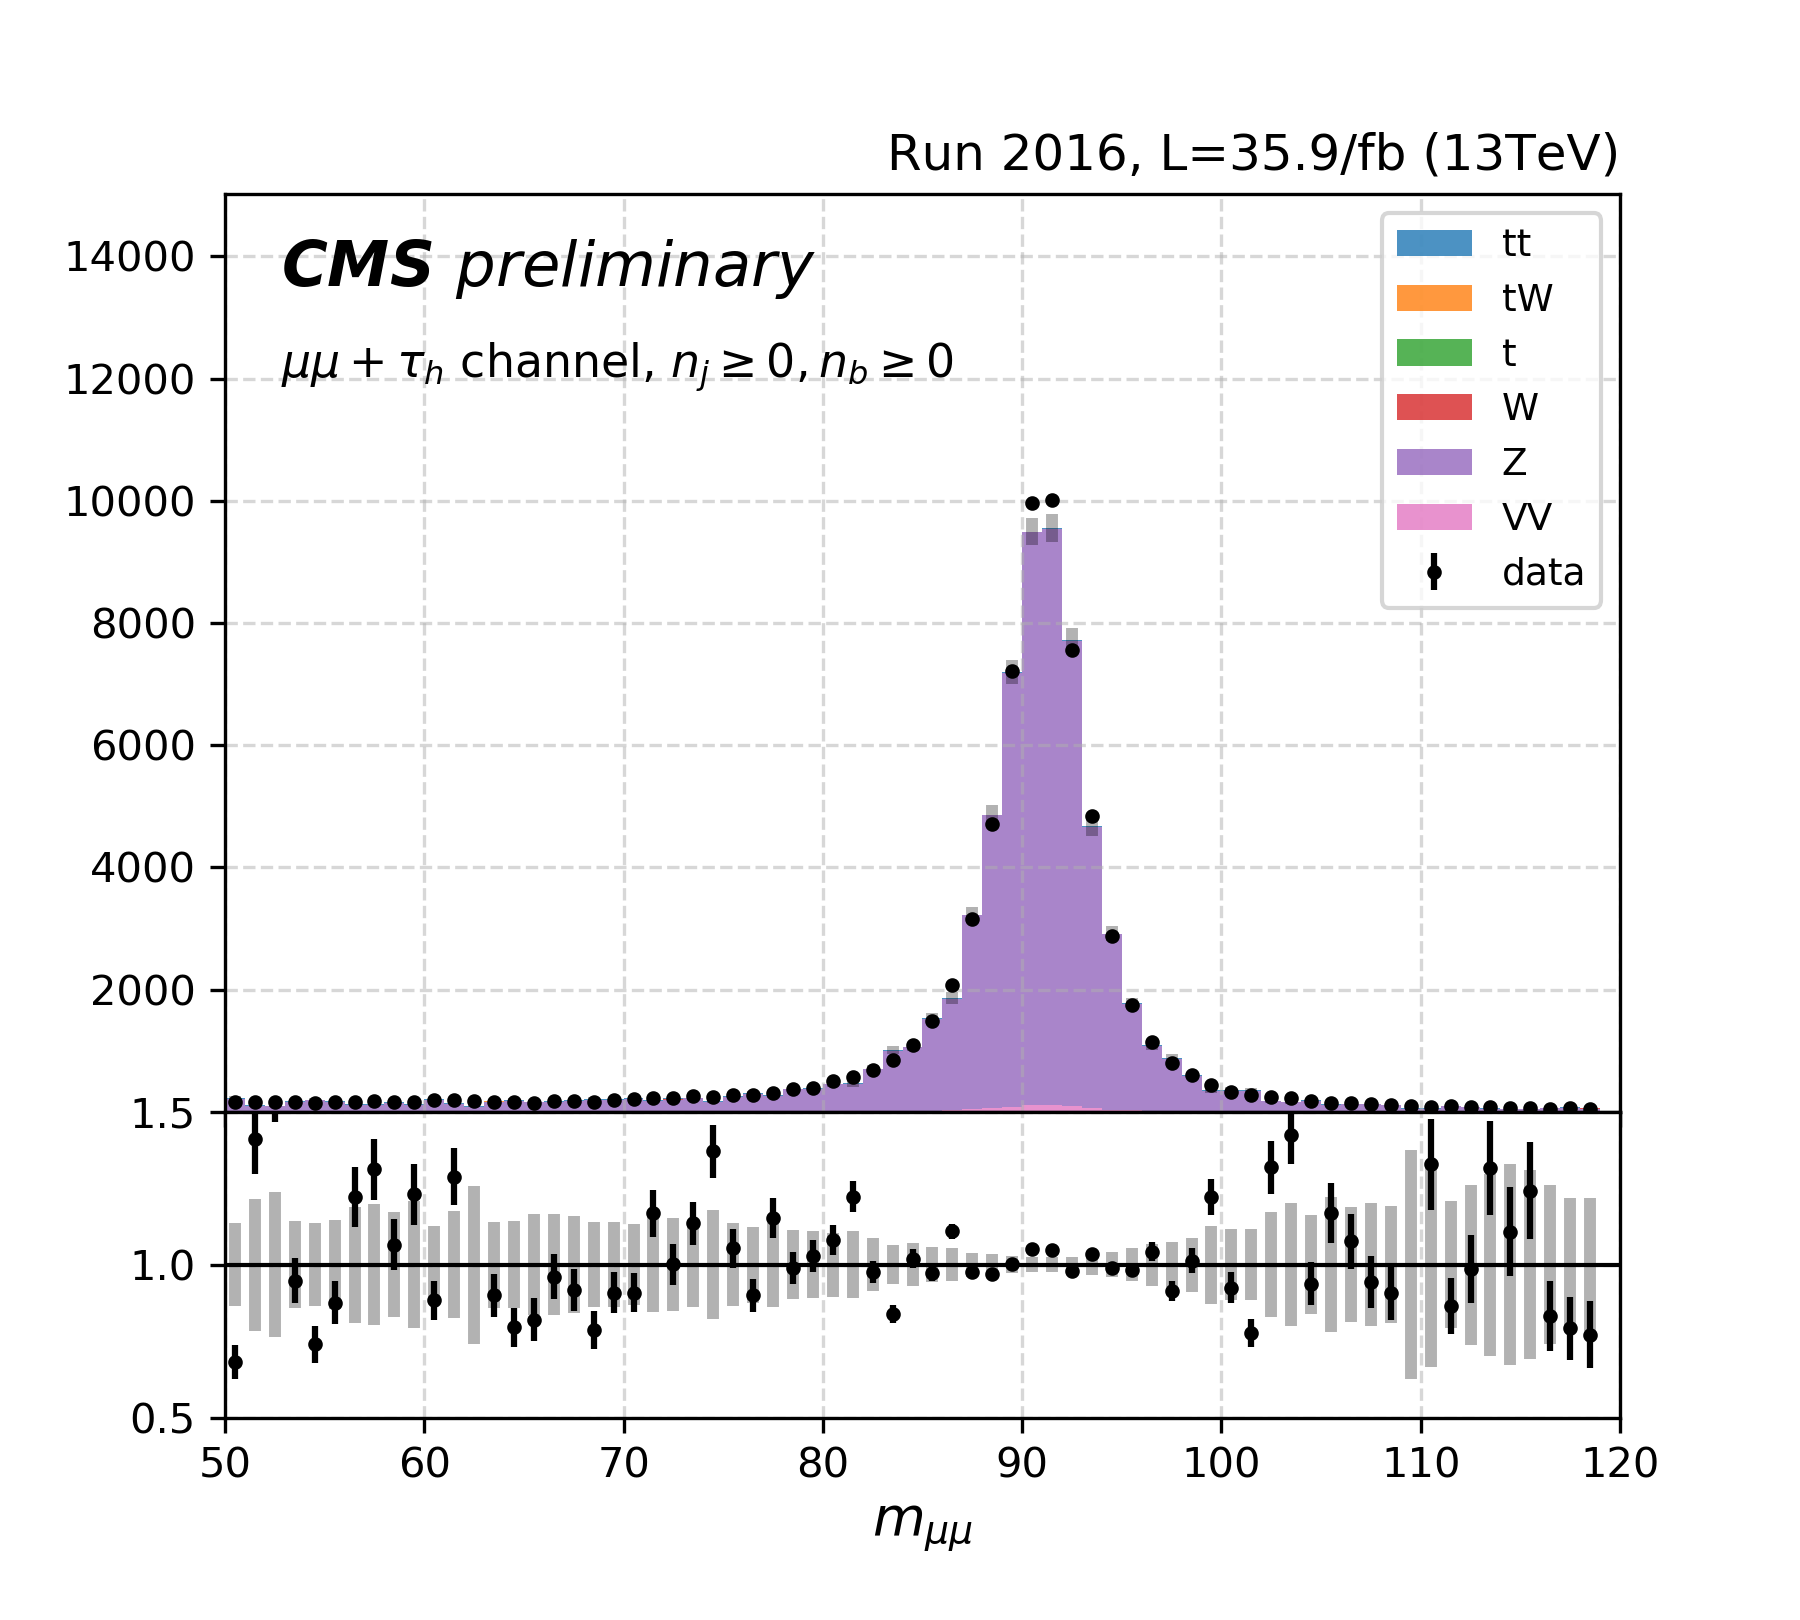
\includegraphics[width=0.4\textwidth]{chapters/Analysis/sectionCalibration/figures/jetToTauh/mumutau_dilepton_mass_pickles_lltauTight.png}
    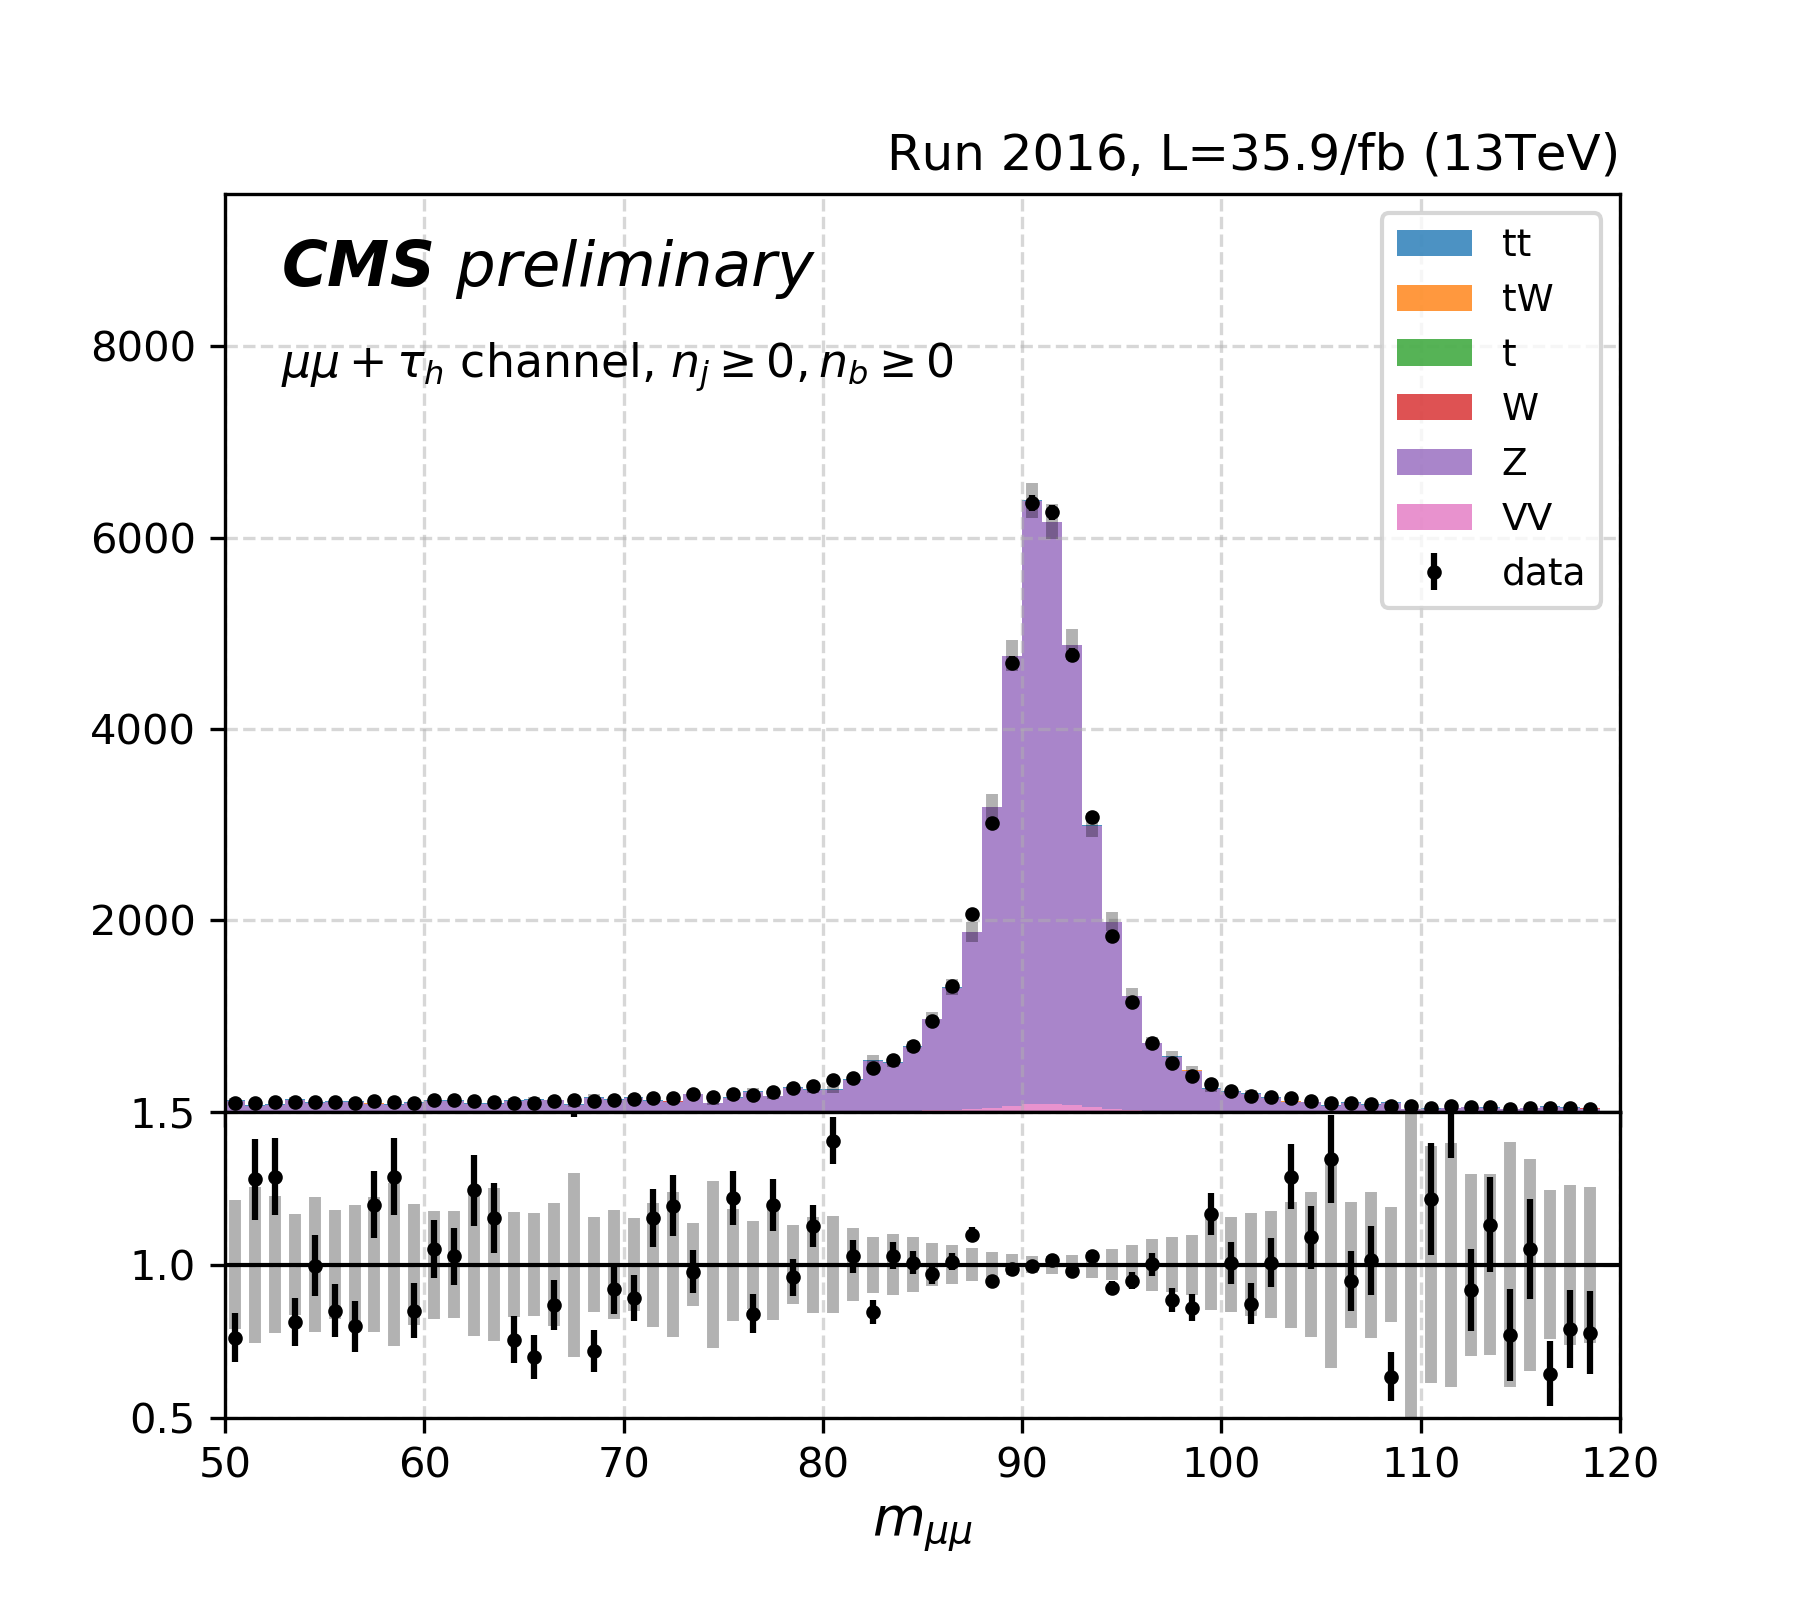
\includegraphics[width=0.4\textwidth]{chapters/Analysis/sectionCalibration/figures/jetToTauh/mumutau_dilepton_mass_pickles_lltauVTight.png}
    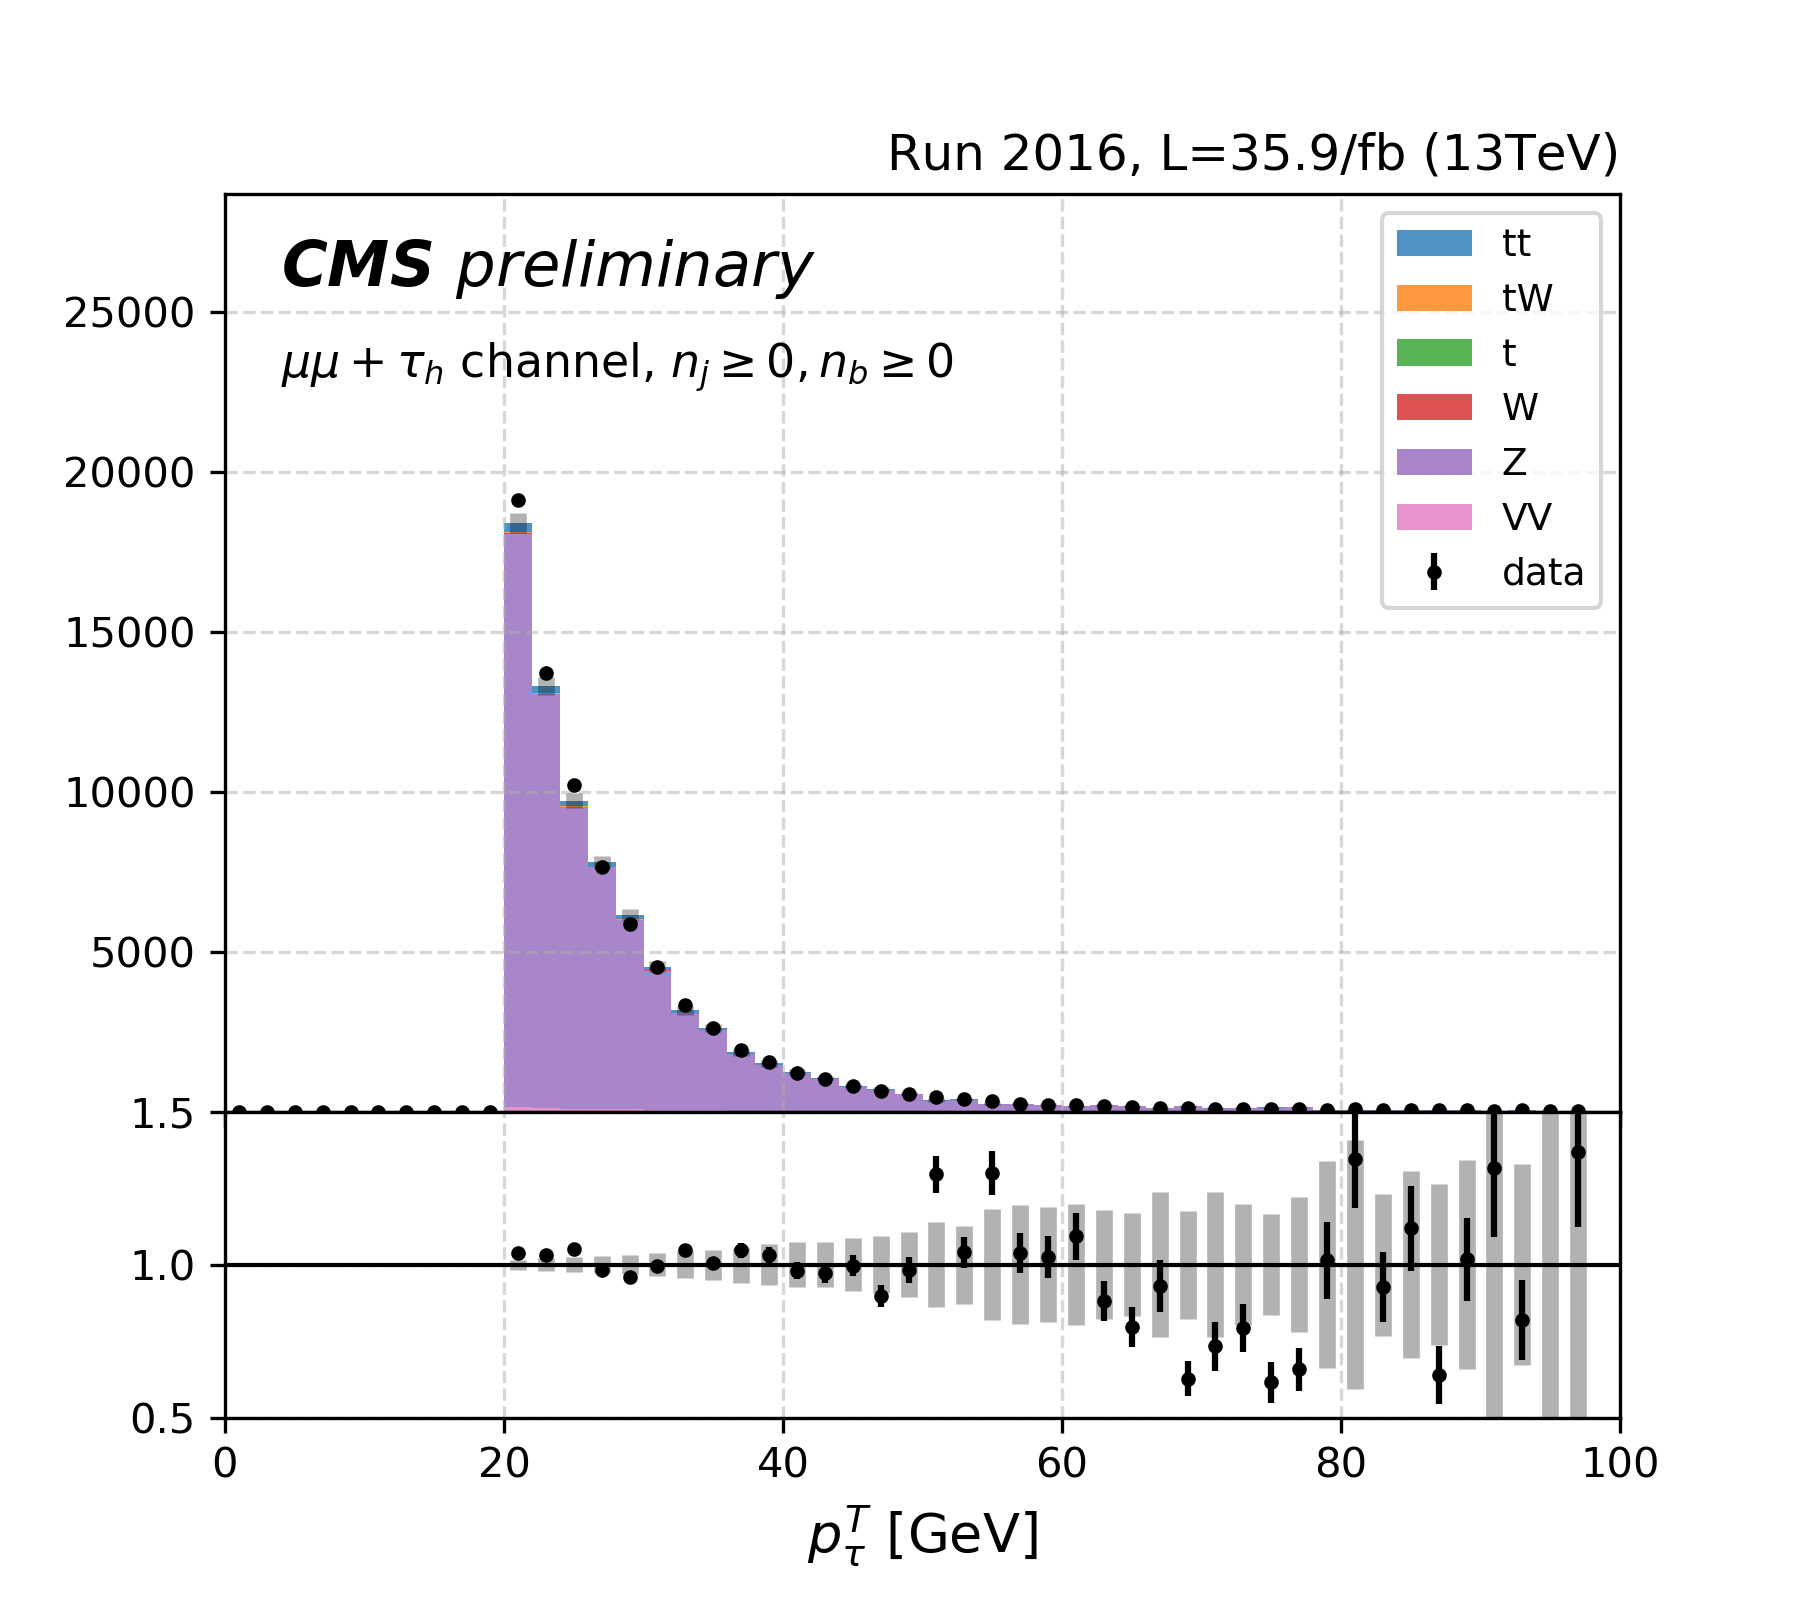
\includegraphics[width=0.4\textwidth]{chapters/Analysis/sectionCalibration/figures/jetToTauh/mumutau_tauPt_pickles_lltauTight.png}
    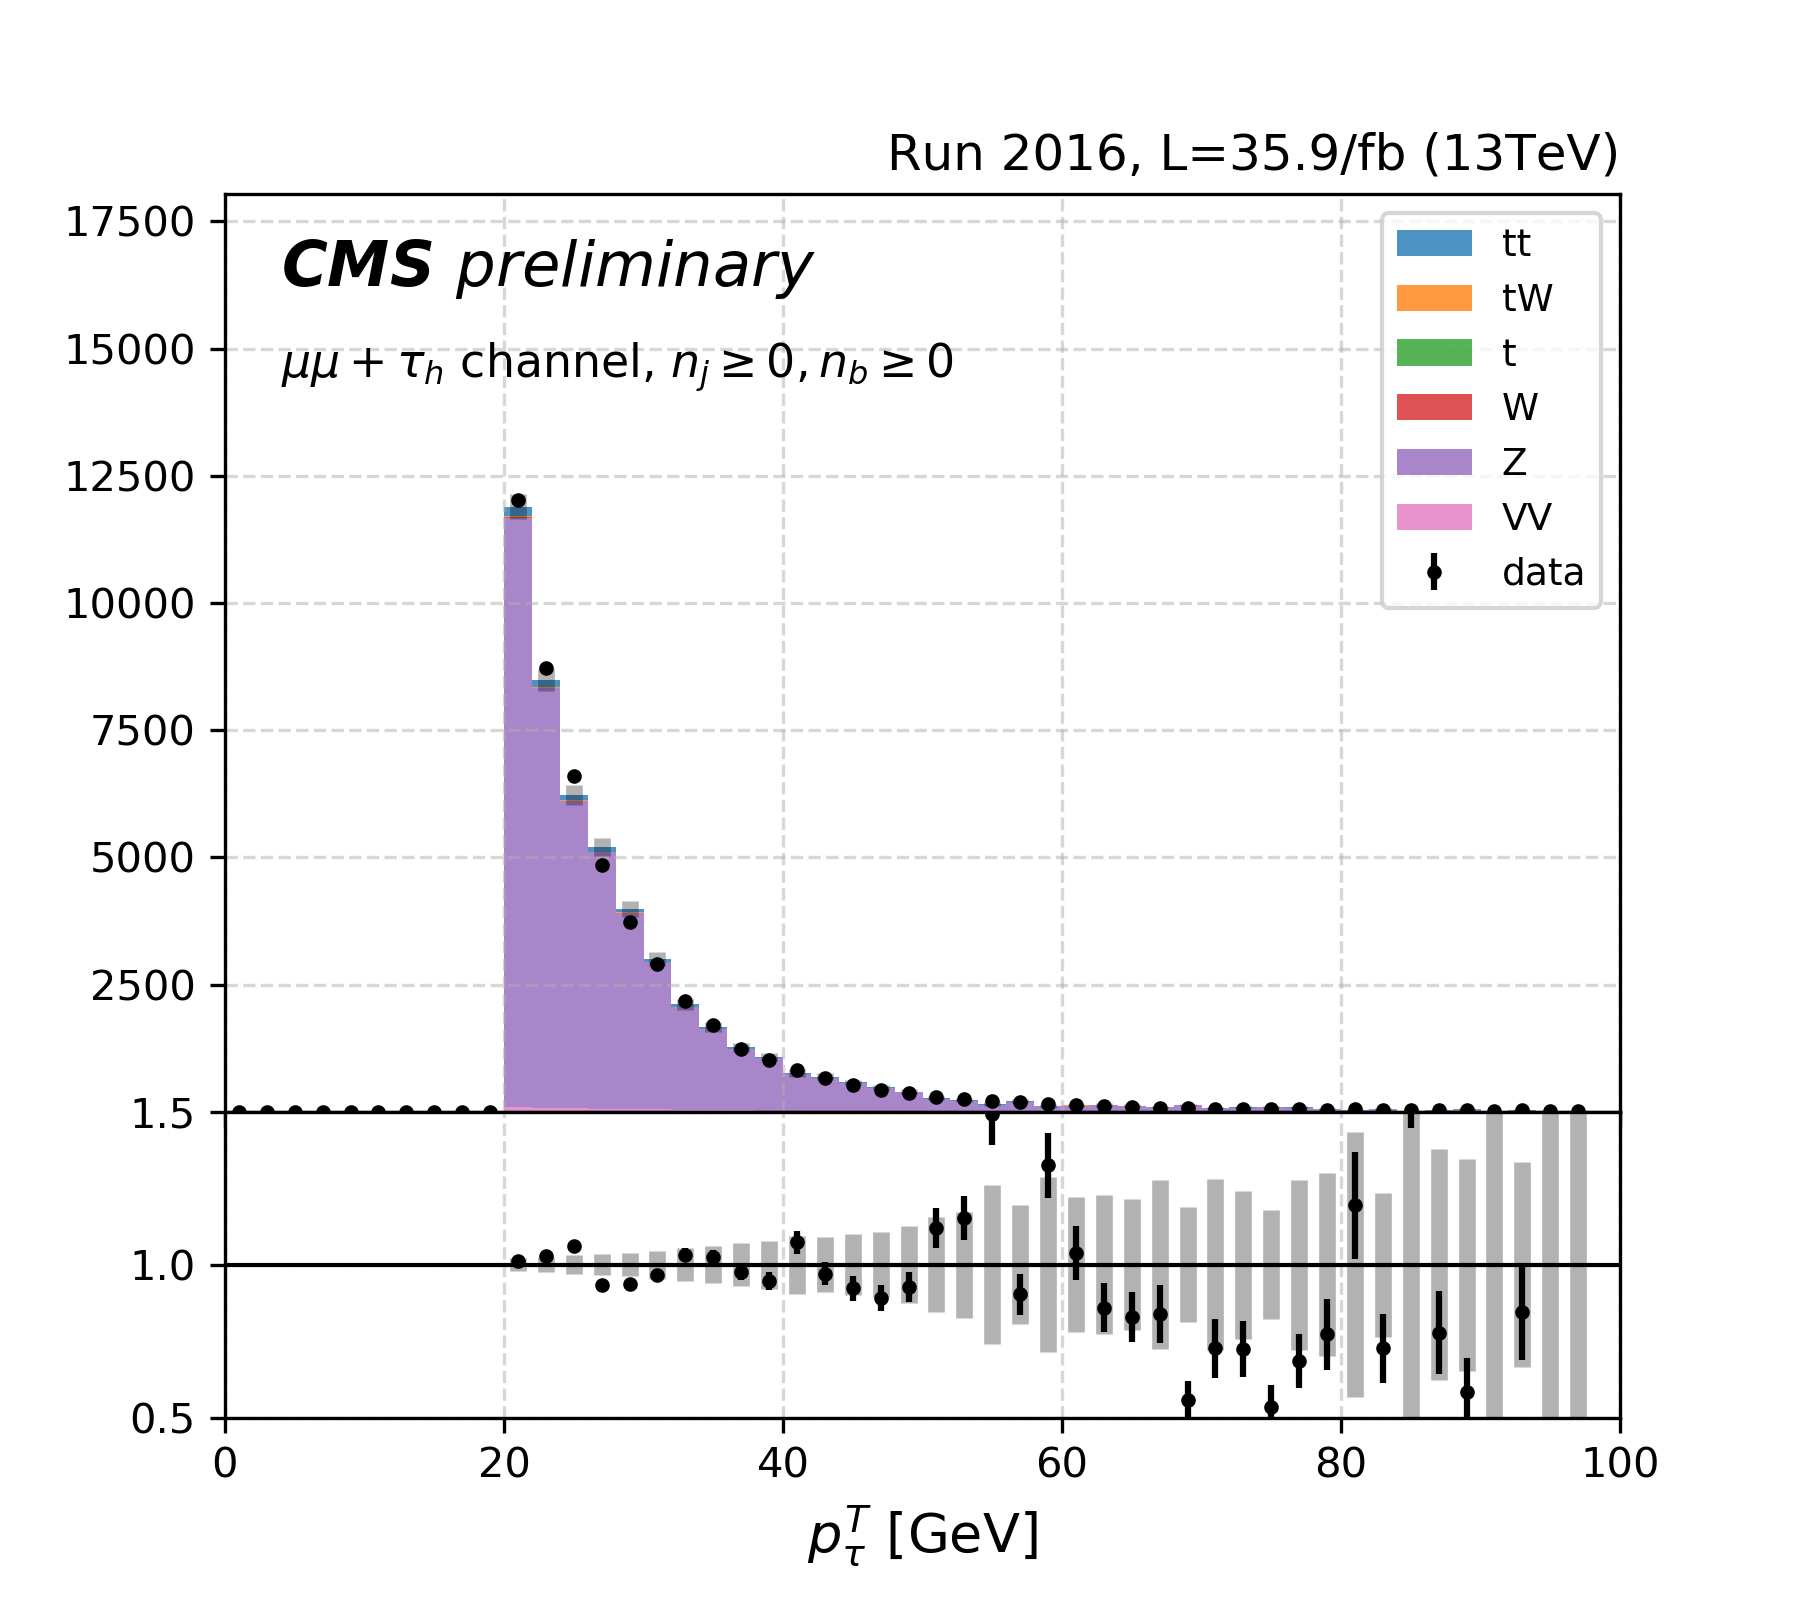
\includegraphics[width=0.4\textwidth]{chapters/Analysis/sectionCalibration/figures/jetToTauh/mumutau_tauPt_pickles_lltauVTight.png}
    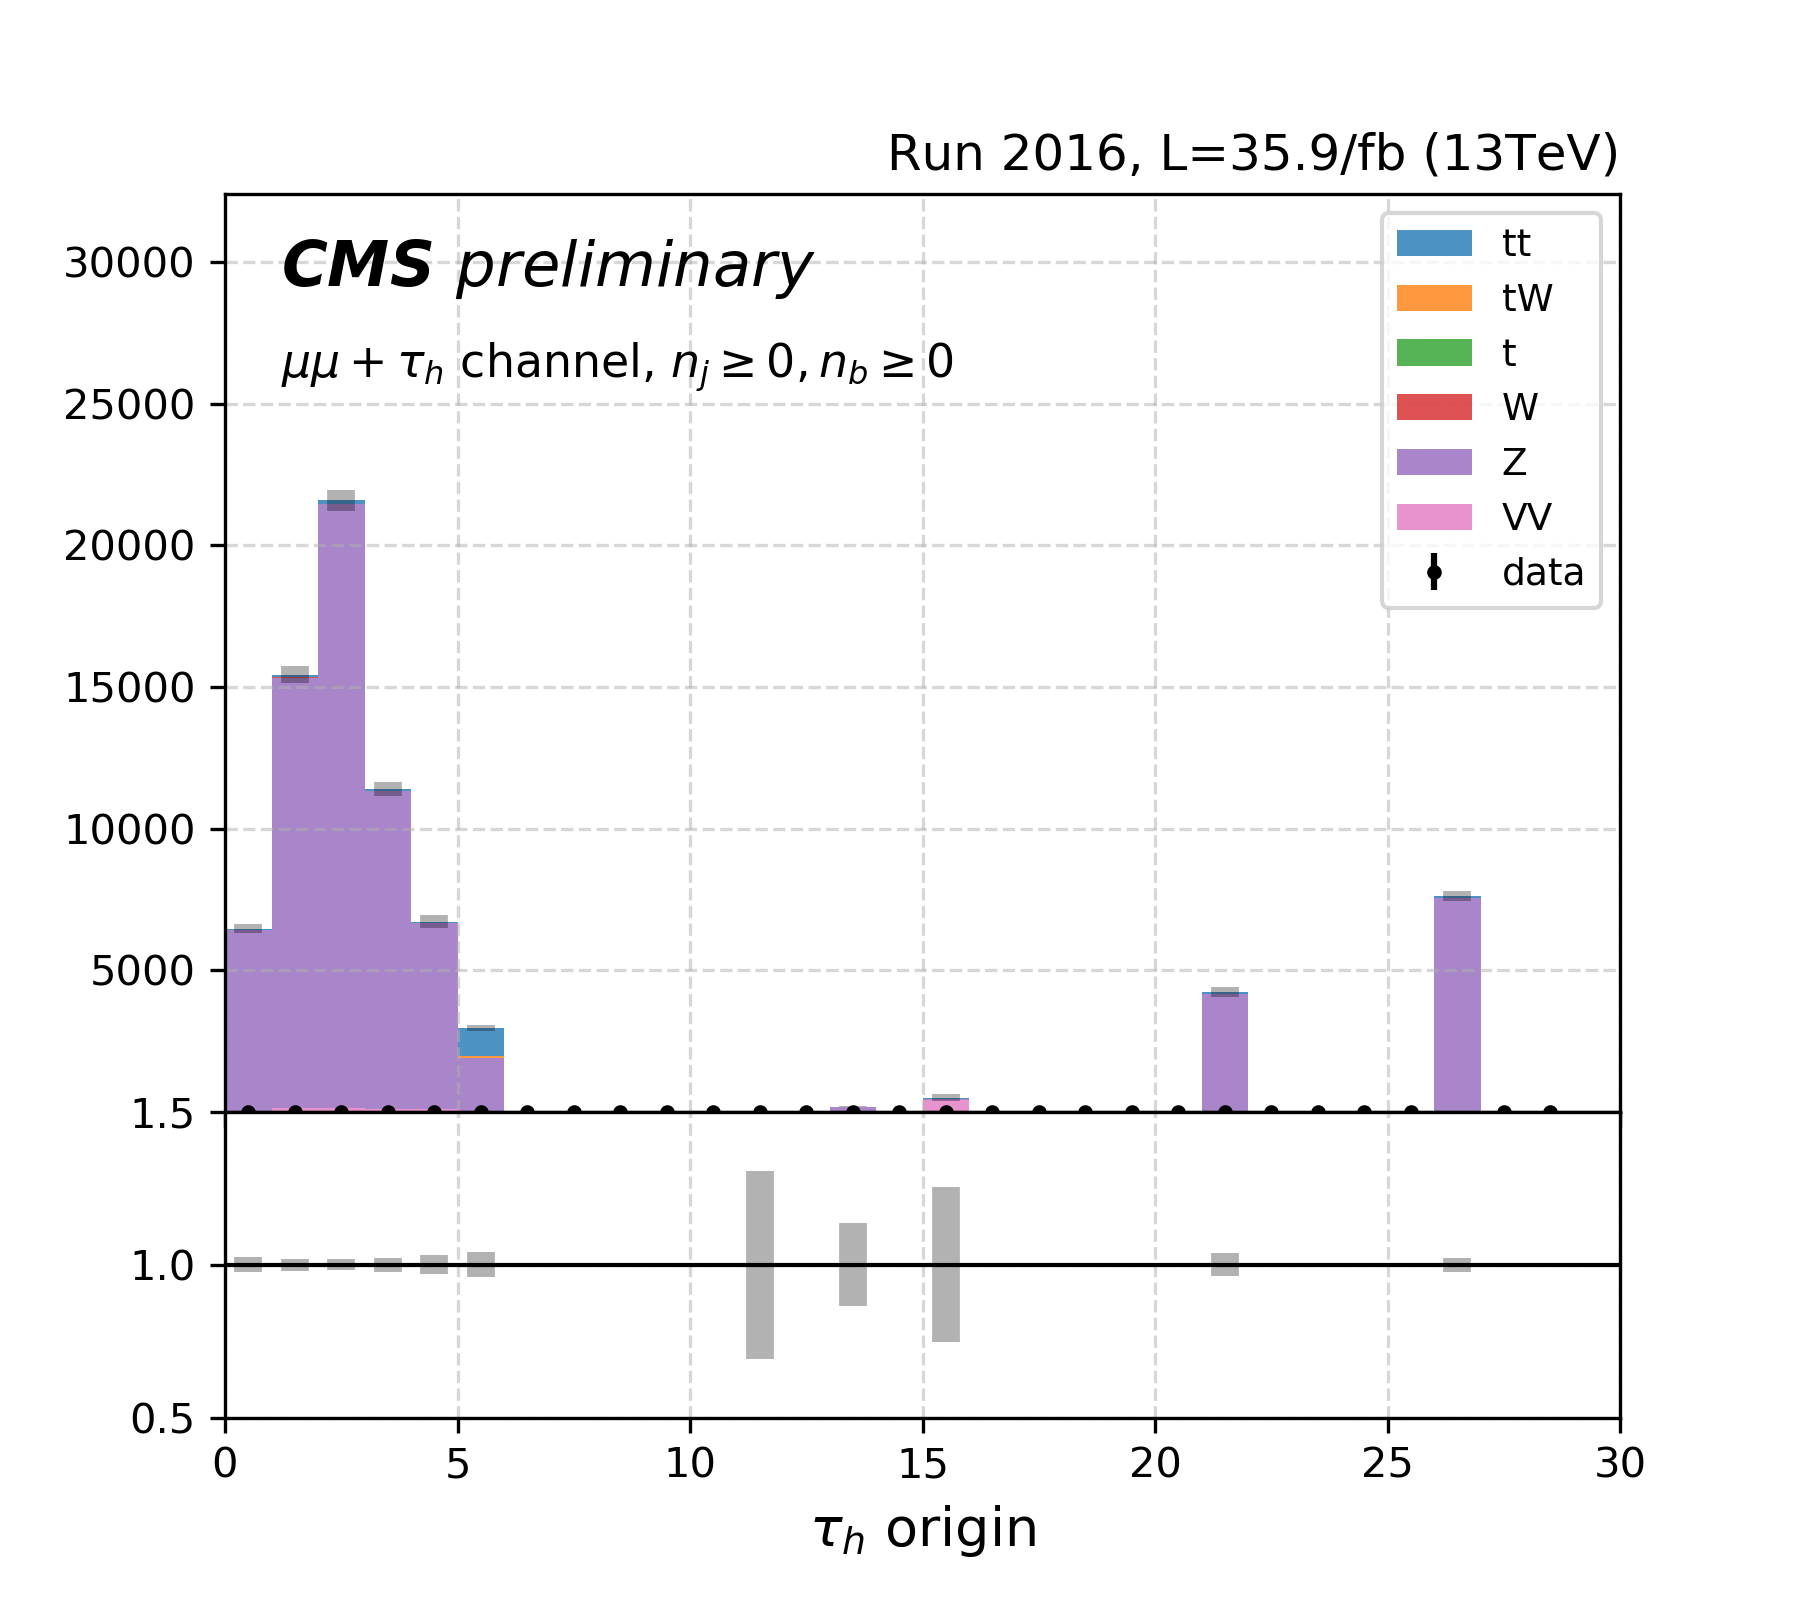
\includegraphics[width=0.4\textwidth]{chapters/Analysis/sectionCalibration/figures/jetToTauh/mumutau_tauGenFlavor_pickles_lltauTight.png}
    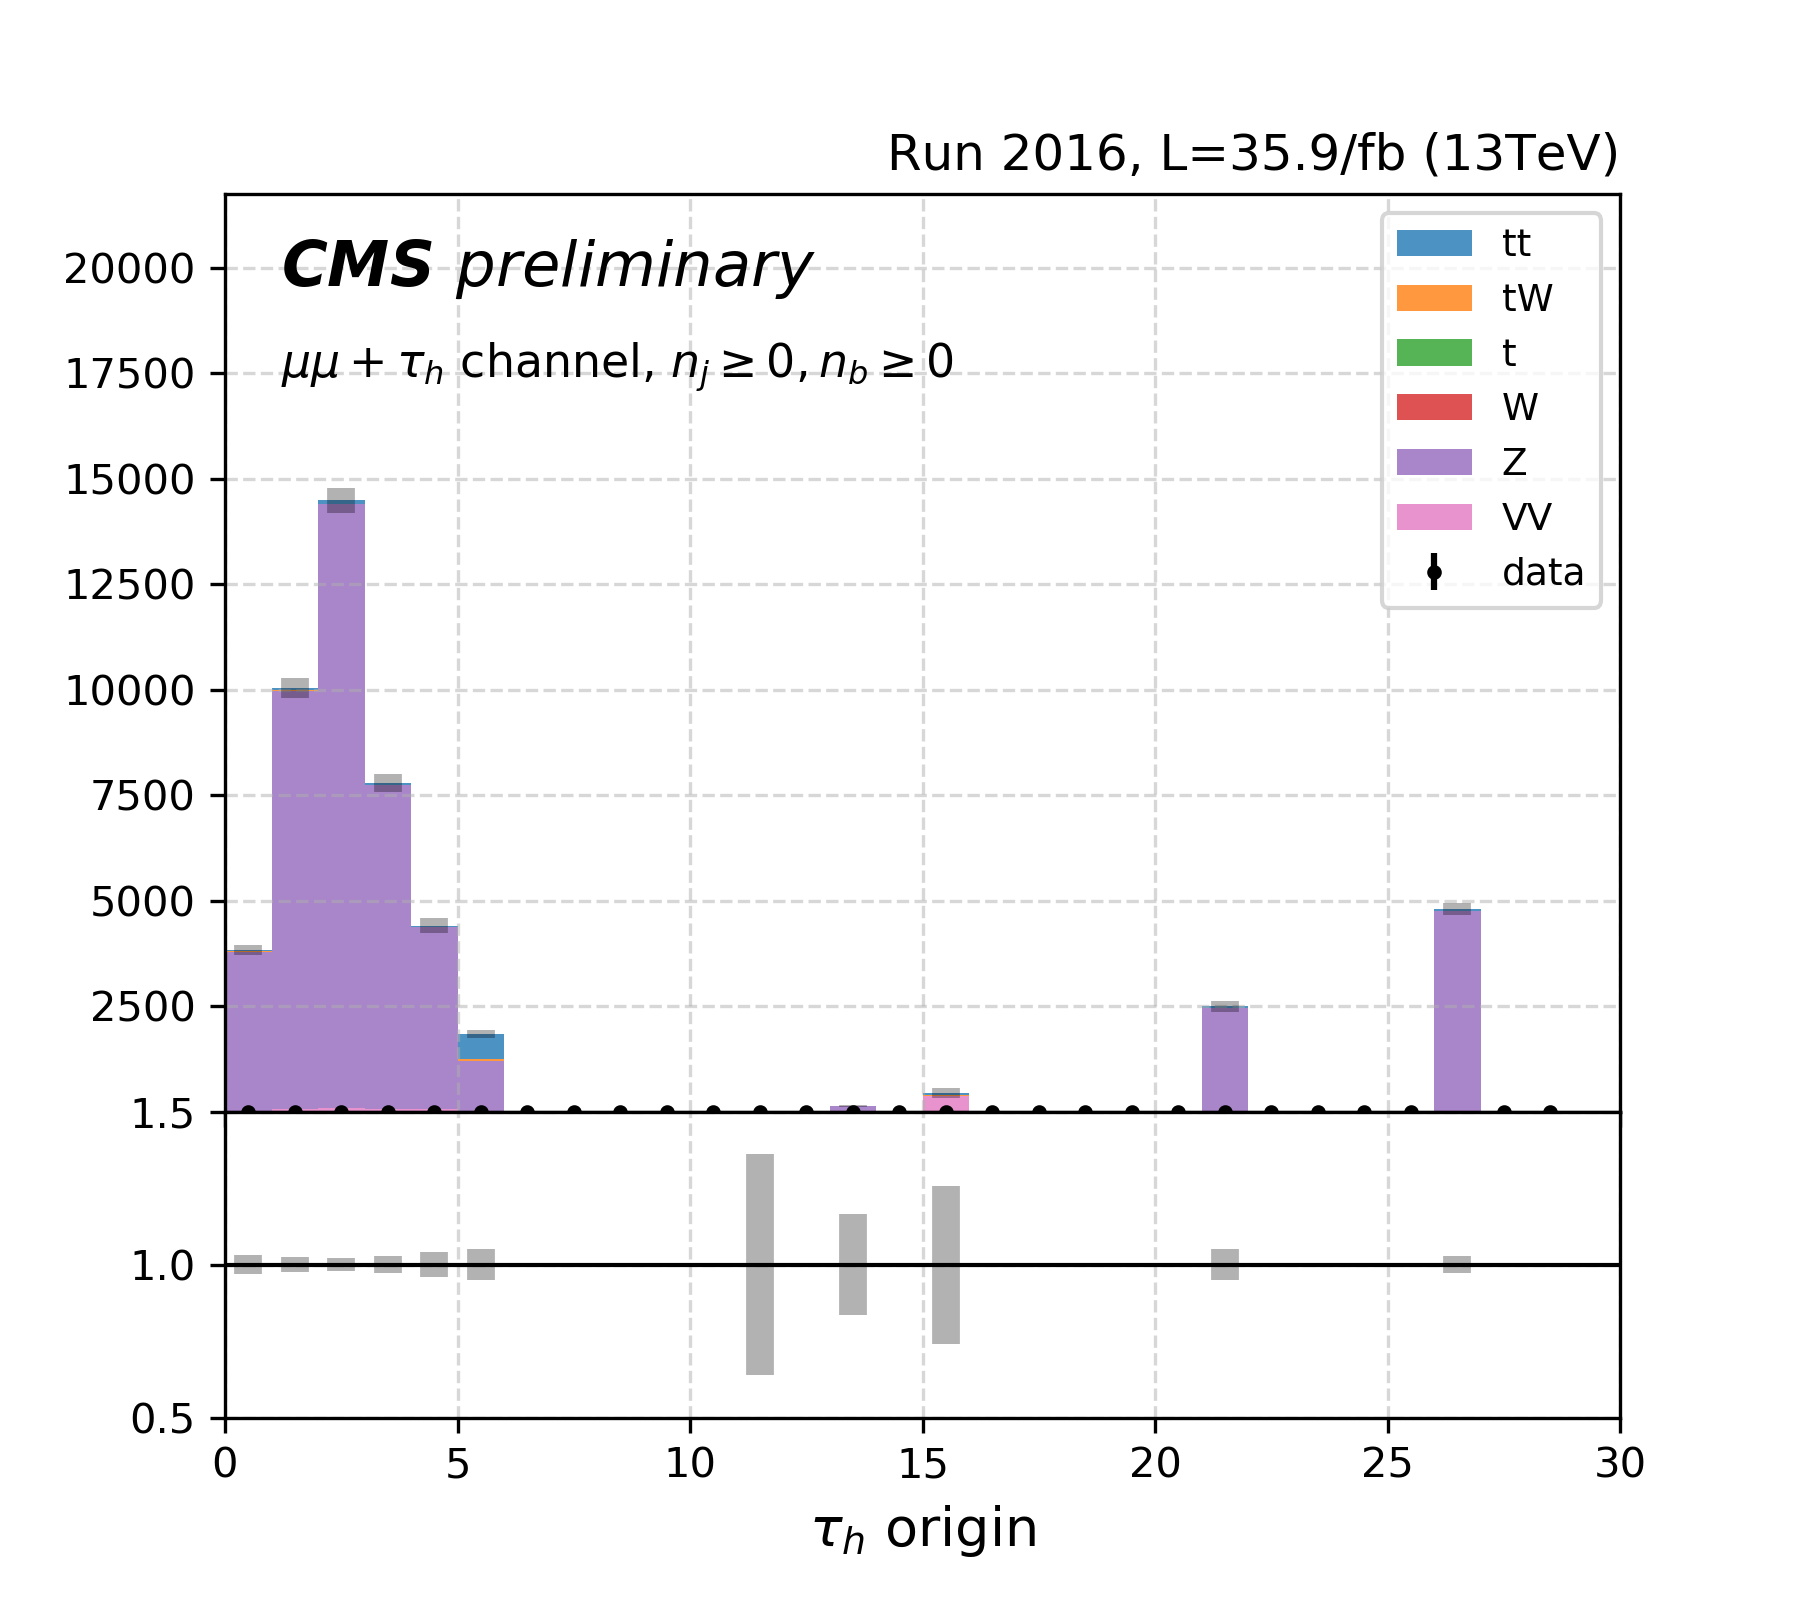
\includegraphics[width=0.4\textwidth]{chapters/Analysis/sectionCalibration/figures/jetToTauh/mumutau_tauGenFlavor_pickles_lltauVTight.png}
    \caption{Distributions of $m_{\mu\mu}$, $\tau_h$ \pt and gen-level $\tau_h$ origin in the $\mu\mu+\tau$ channel. The left and right column shows the Tight and VTight $\tau_h$ WP respectively.}
    \label{fig:appendix:fakeTauId:mumutau}
\end{figure}


\begin{figure}
    \centering
    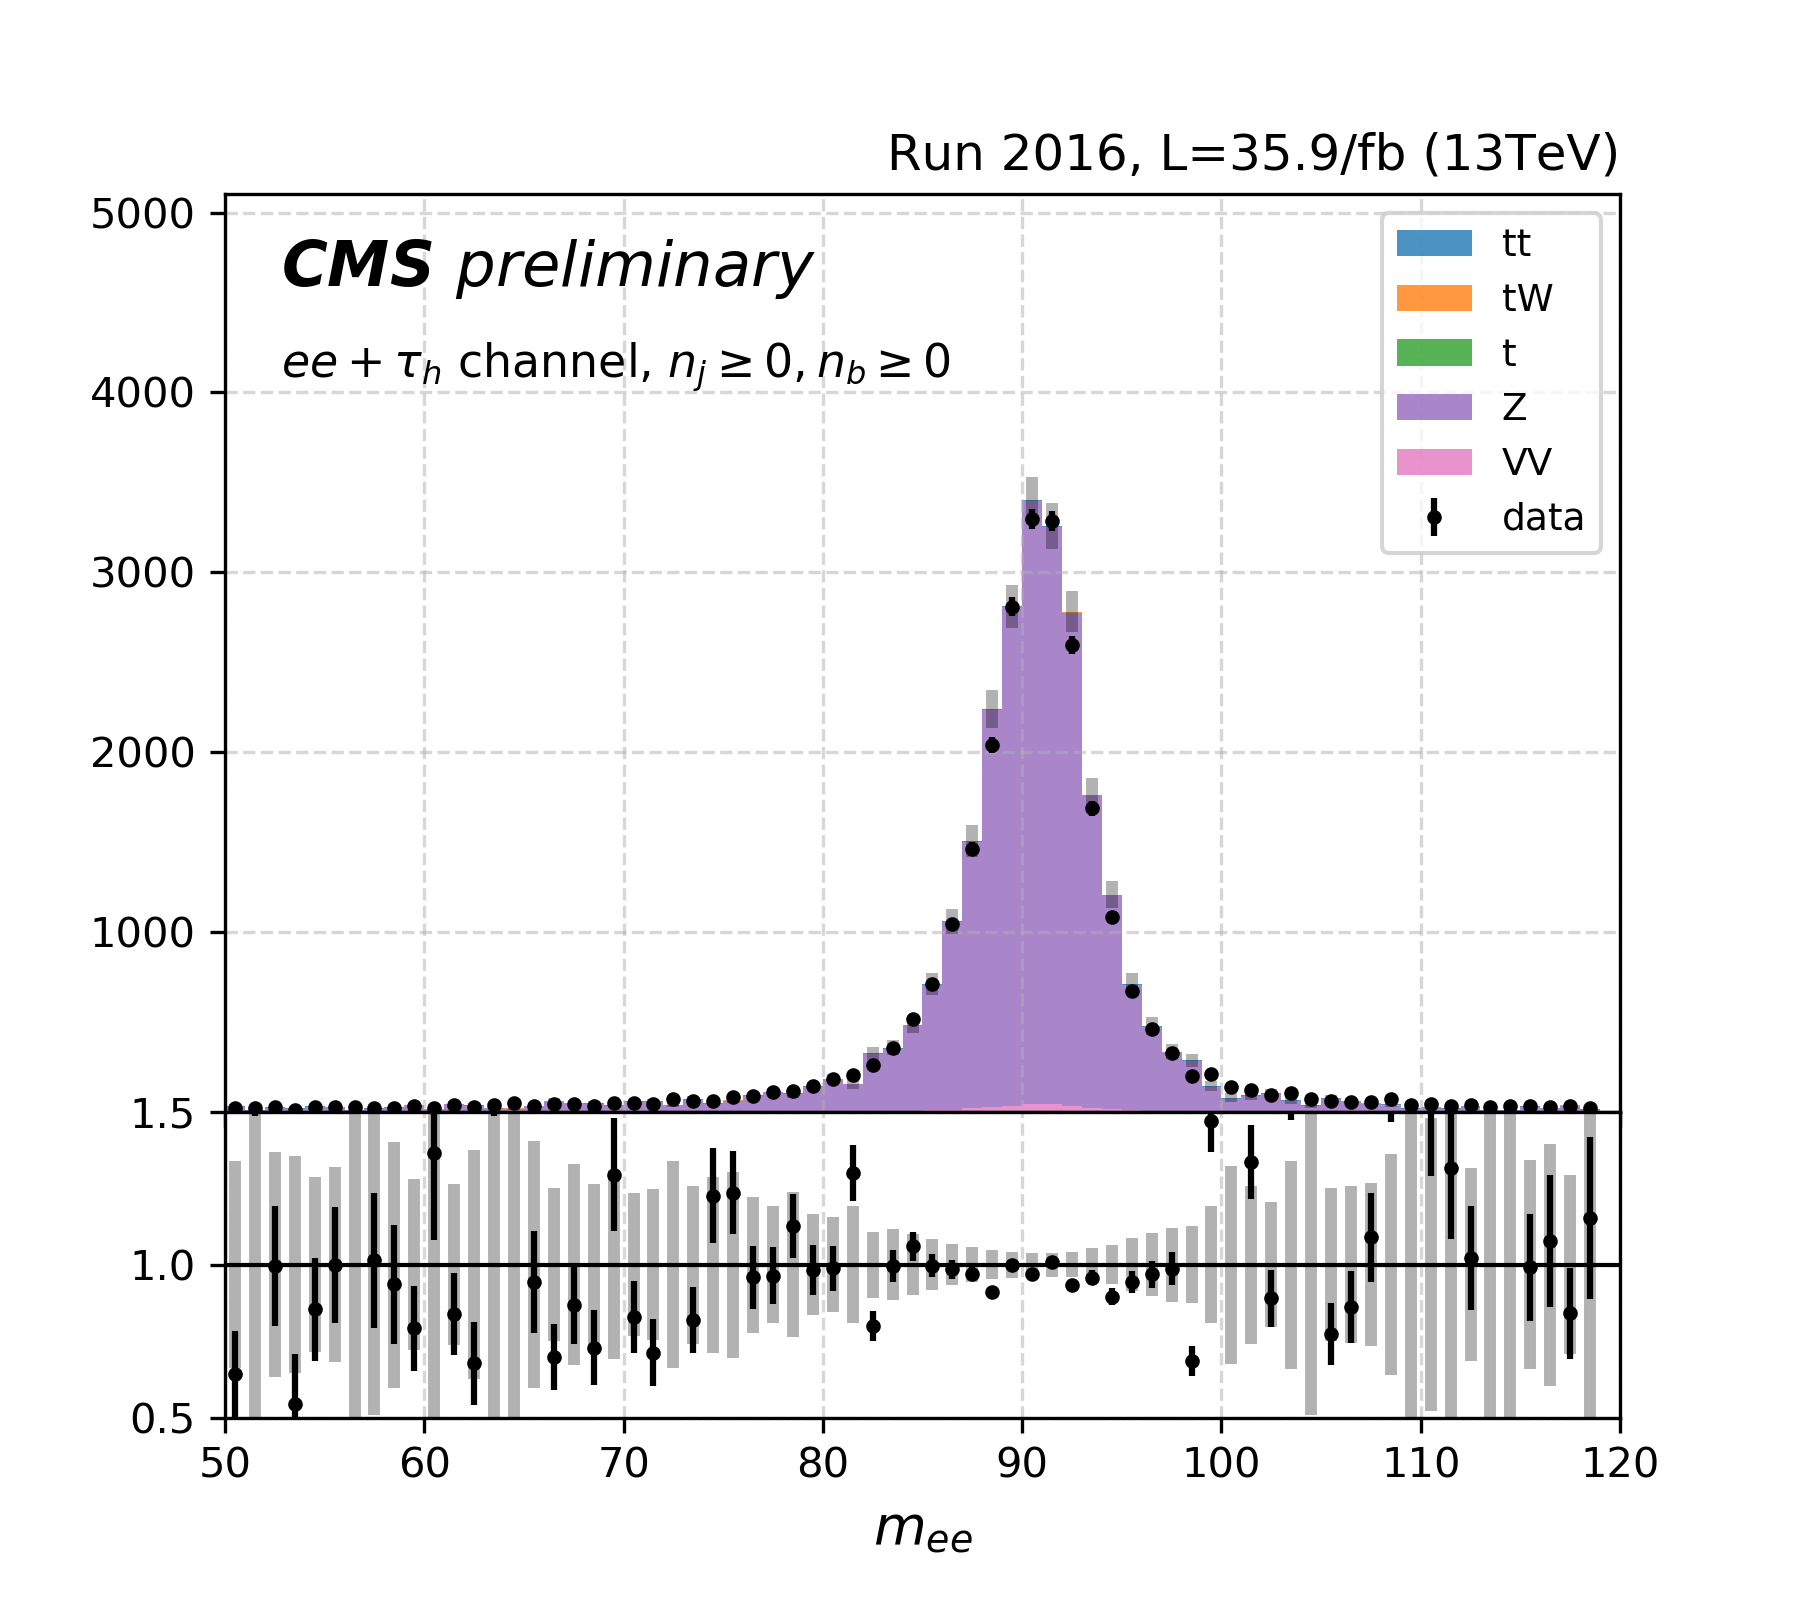
\includegraphics[width=0.4\textwidth]{chapters/Analysis/sectionCalibration/figures/jetToTauh/eetau_dilepton_mass_pickles_lltauTight.png}
    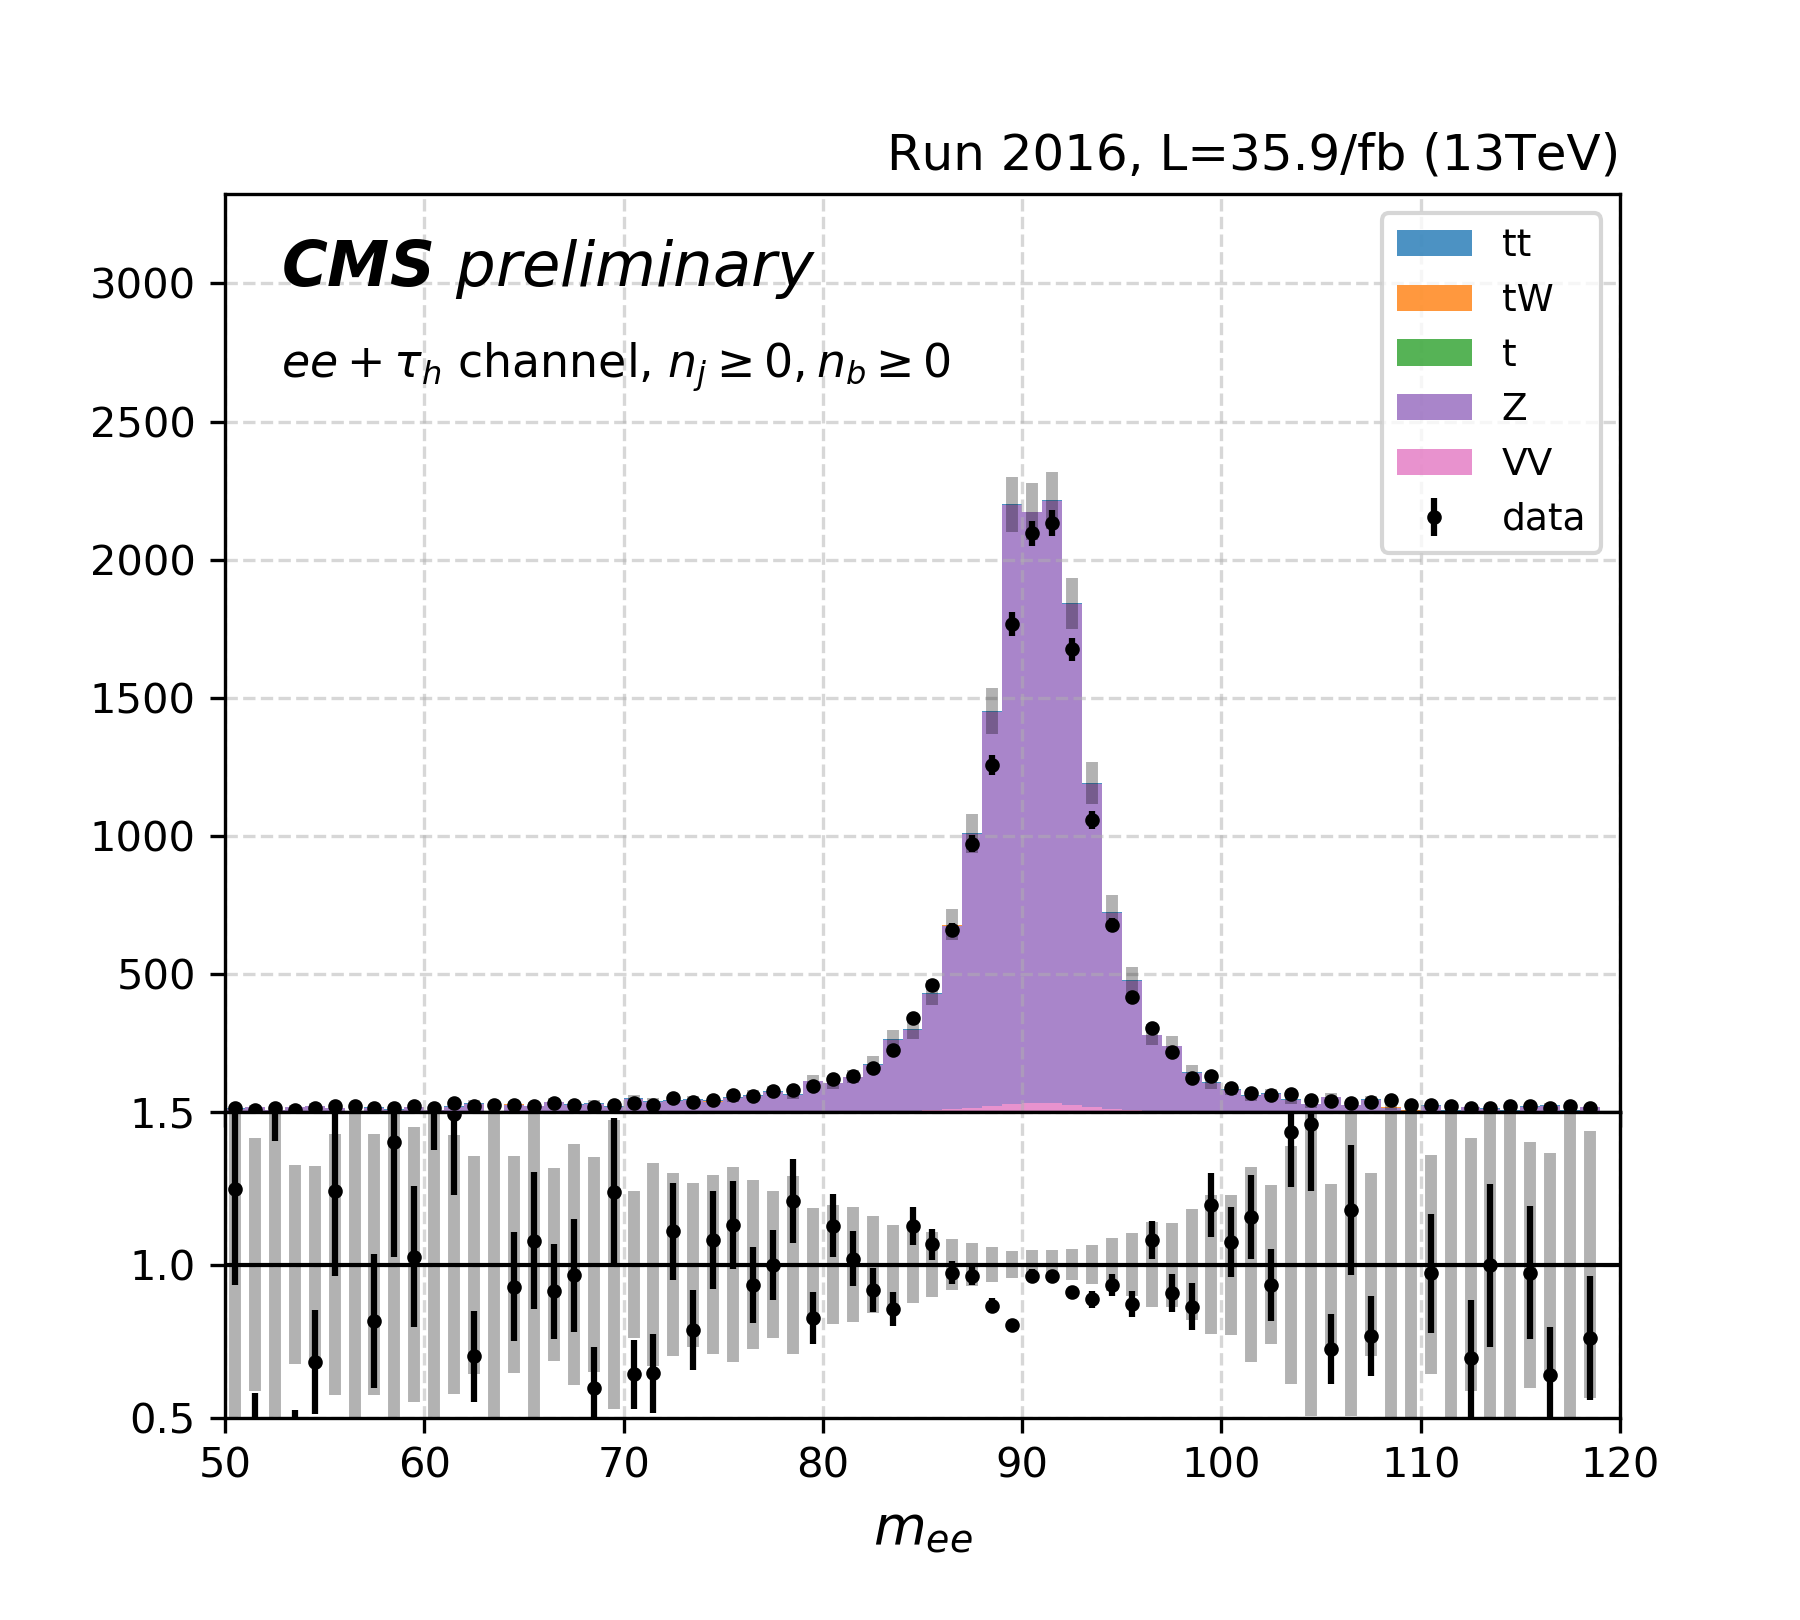
\includegraphics[width=0.4\textwidth]{chapters/Analysis/sectionCalibration/figures/jetToTauh/eetau_dilepton_mass_pickles_lltauVTight.png}
    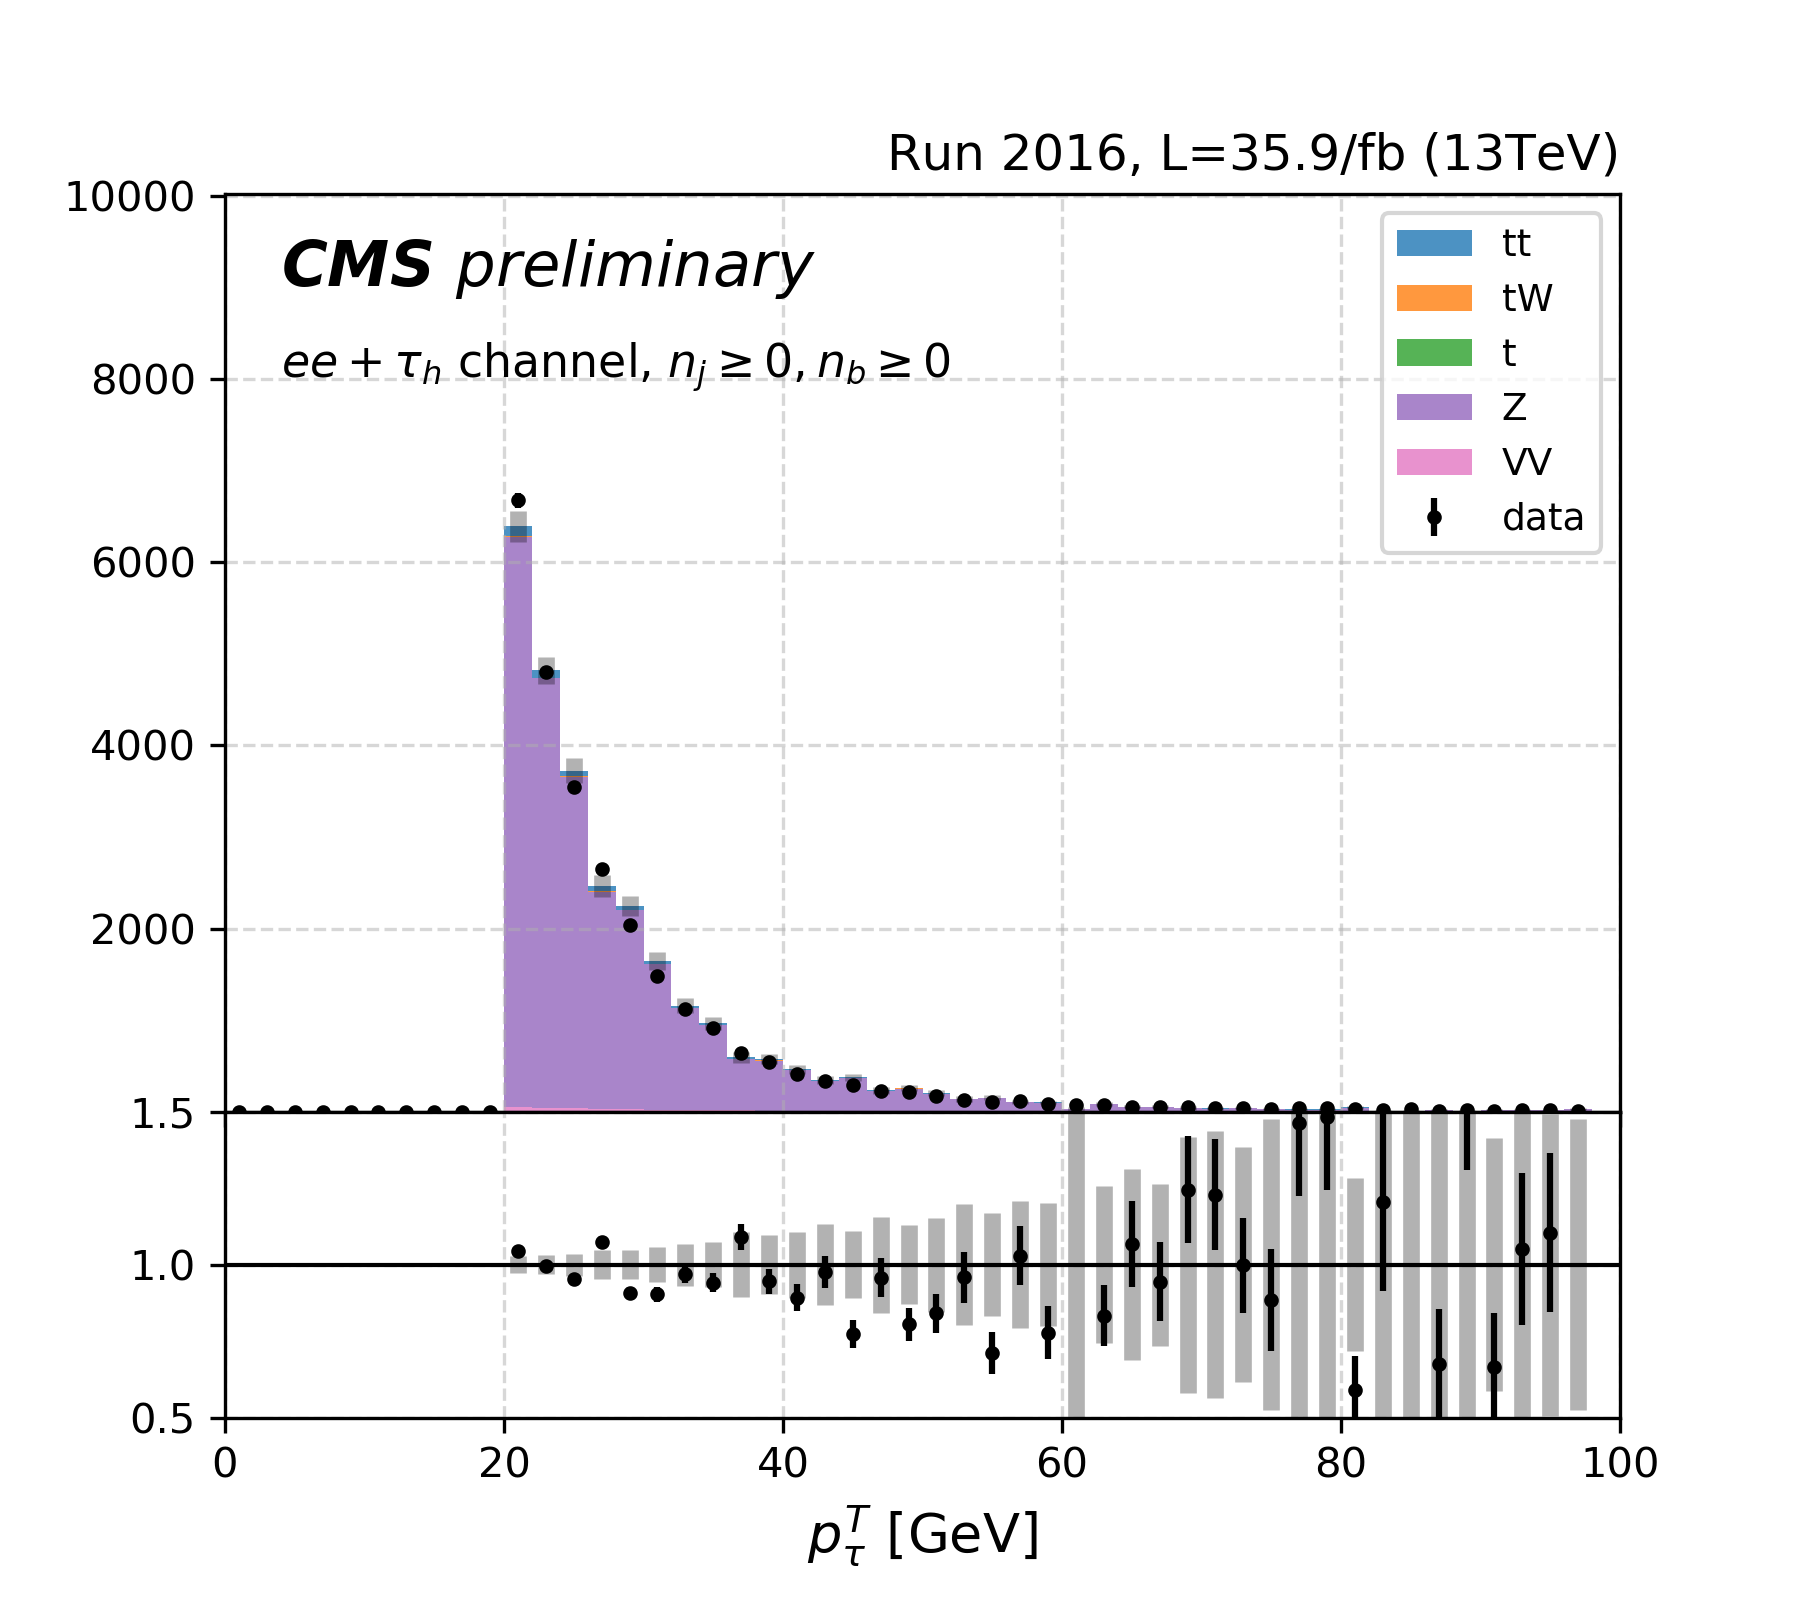
\includegraphics[width=0.4\textwidth]{chapters/Analysis/sectionCalibration/figures/jetToTauh/eetau_tauPt_pickles_lltauTight.png}
    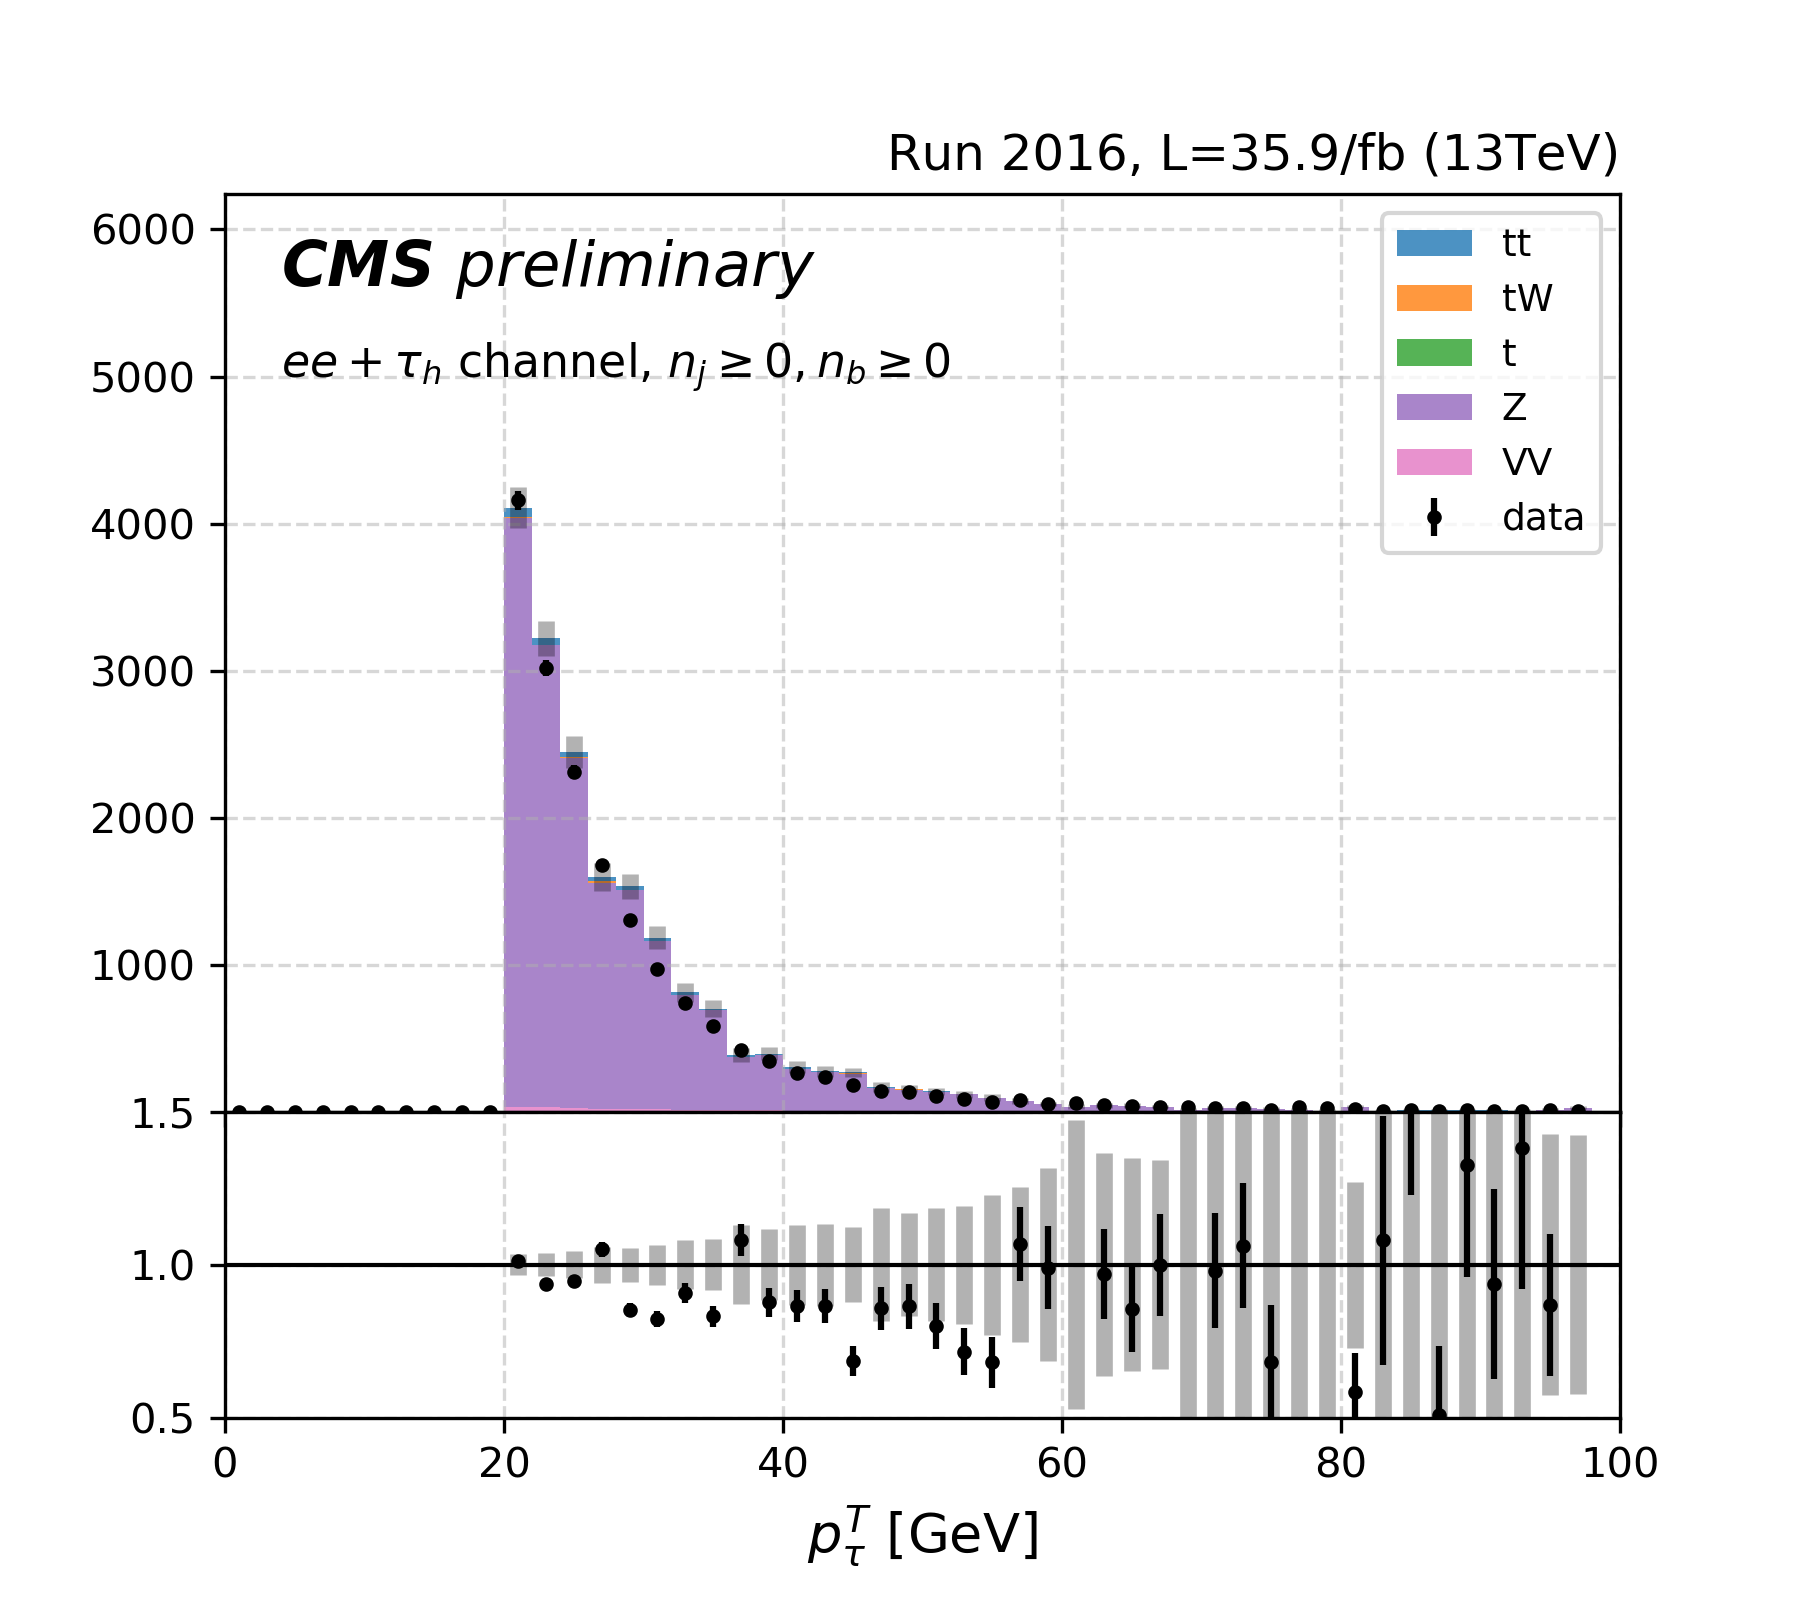
\includegraphics[width=0.4\textwidth]{chapters/Analysis/sectionCalibration/figures/jetToTauh/eetau_tauPt_pickles_lltauVTight.png}
    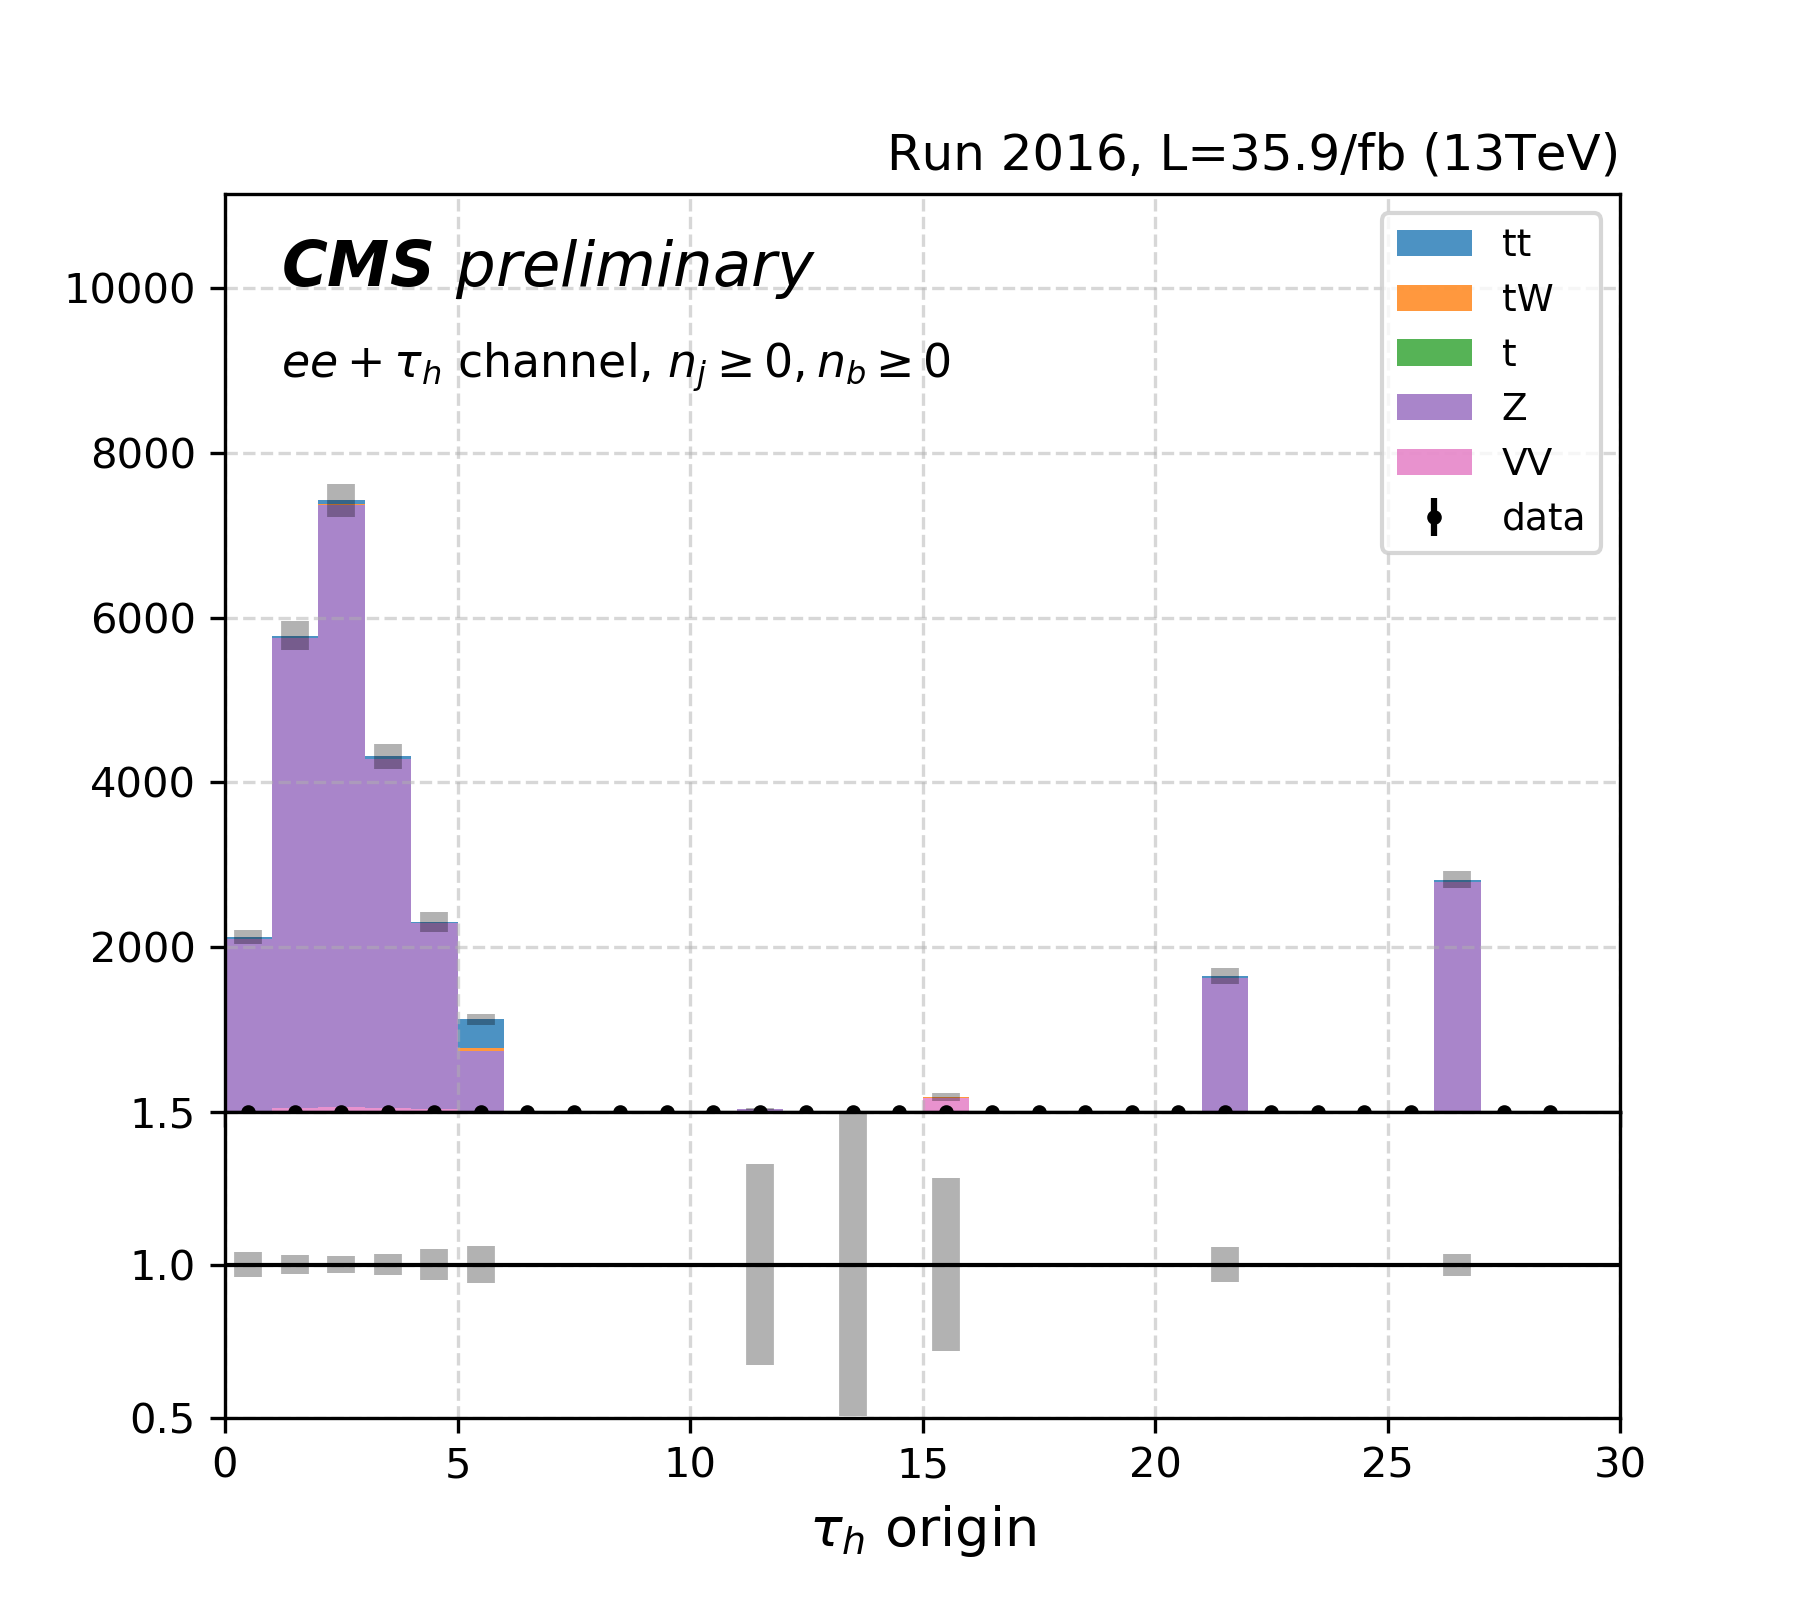
\includegraphics[width=0.4\textwidth]{chapters/Analysis/sectionCalibration/figures/jetToTauh/eetau_tauGenFlavor_pickles_lltauTight.png}
    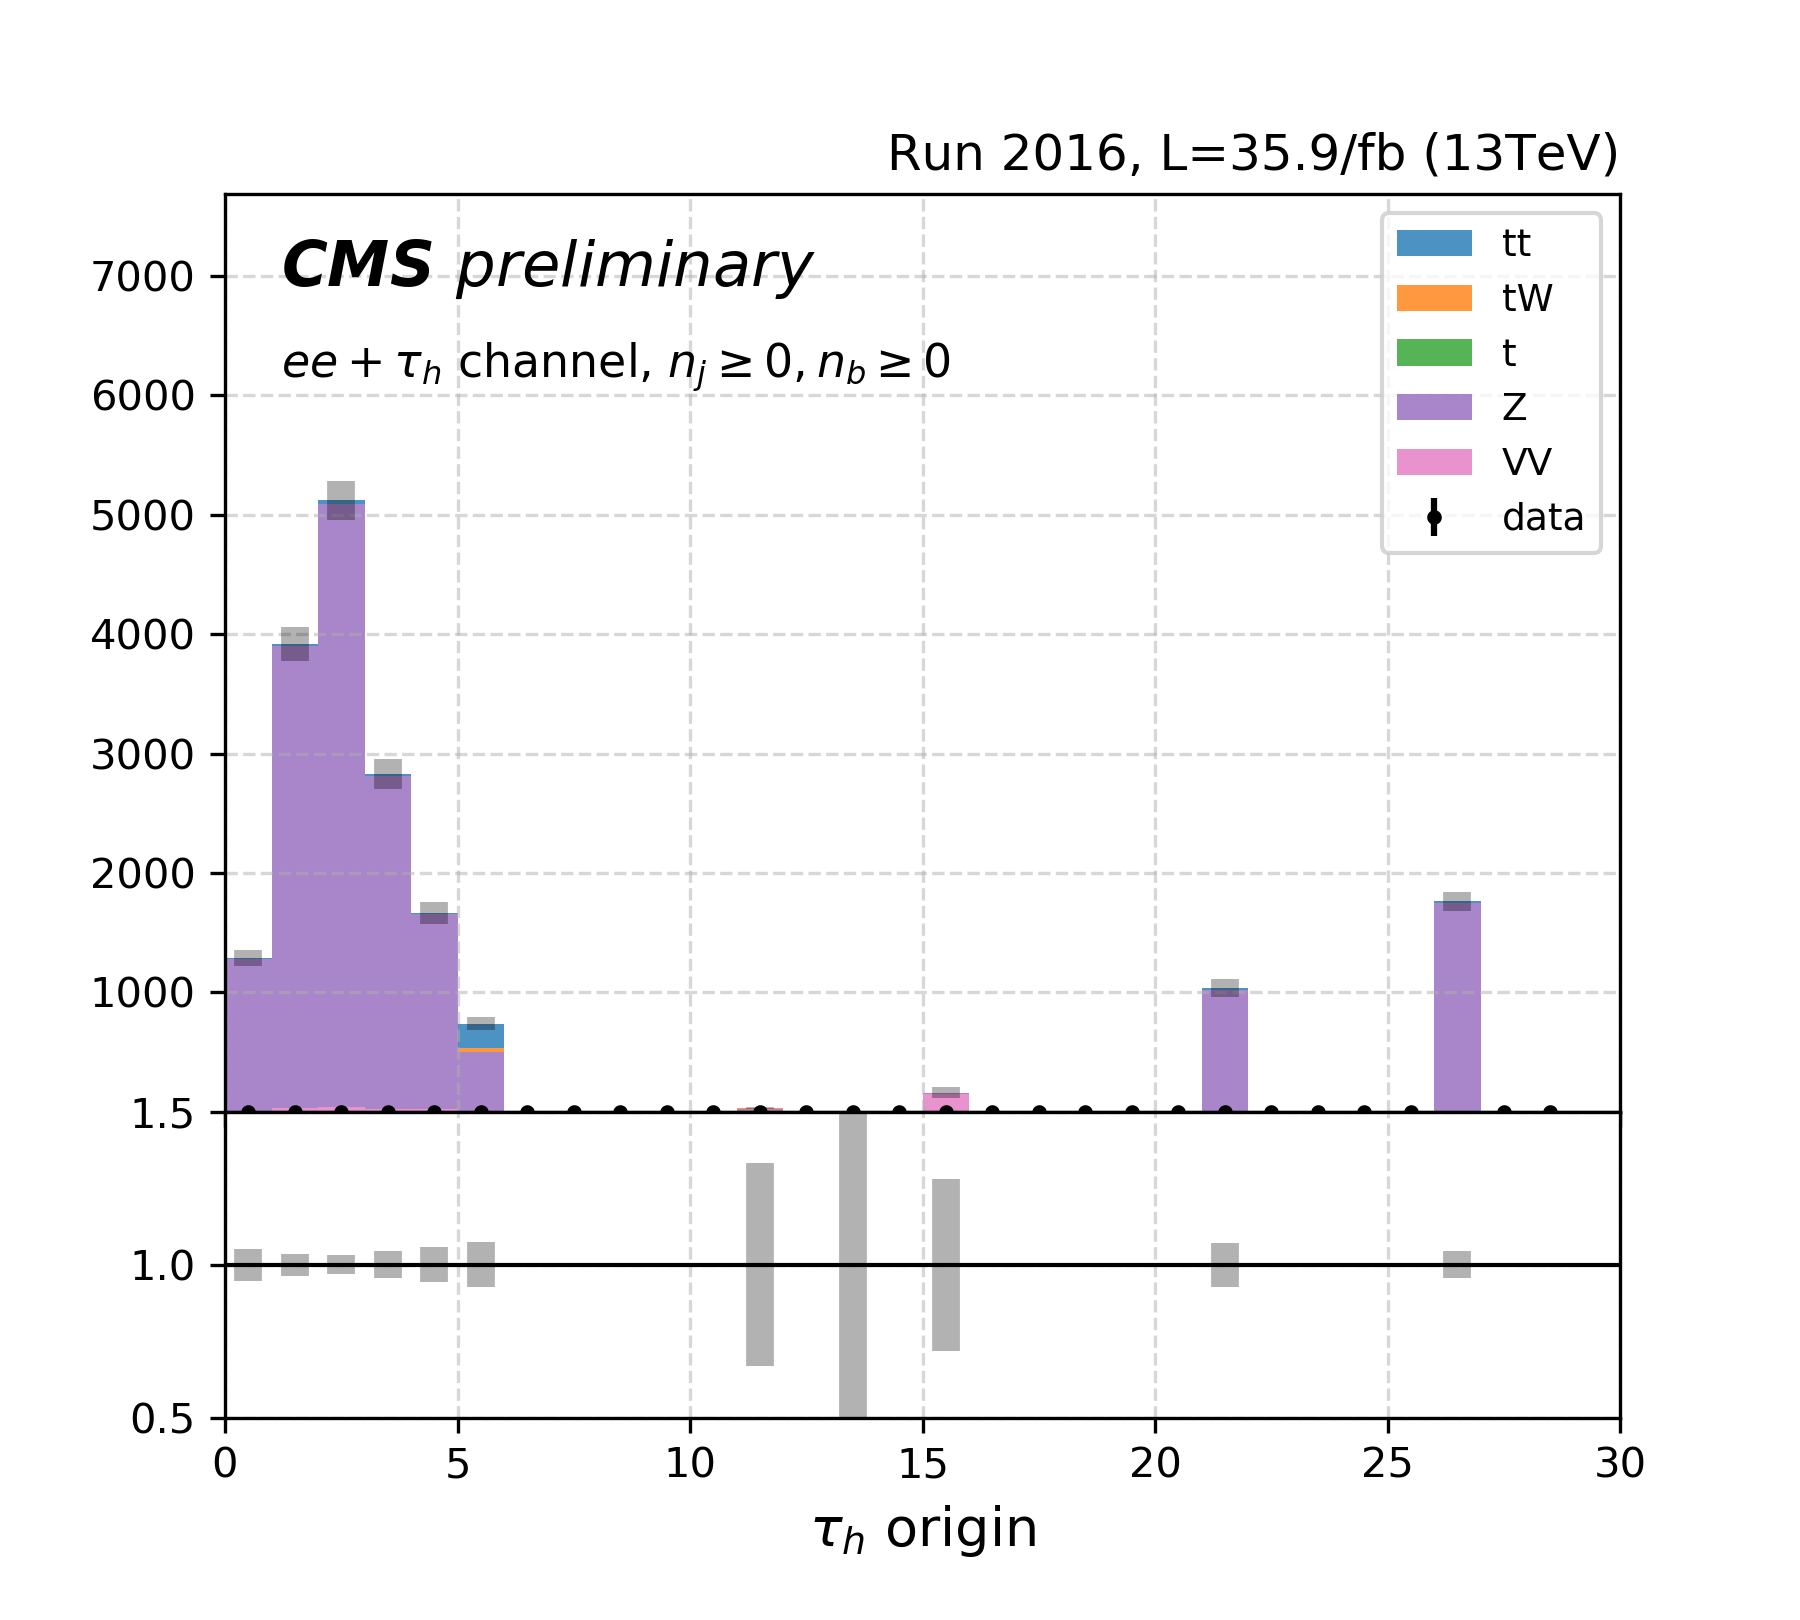
\includegraphics[width=0.4\textwidth]{chapters/Analysis/sectionCalibration/figures/jetToTauh/eetau_tauGenFlavor_pickles_lltauVTight.png}
    \caption{Distributions of $m_{ee}$, $\tau_h$ \pt and gen-level $\tau_h$ origin in the $ee+\tau$ channel. The left and right column shows the Tight and VTight $\tau_h$ WP respectively.}
    \label{fig:appendix:fakeTauId:eetau}
\end{figure}


The \pt spectrum of $\tau_h$ in $\mu\mu+\tau_h$, $ee+\tau_h$ and $e\mu+\tau_h$ final states are shown in figure~\ref{fig:misidprefit}. Because jet modeling of Z+jet is off in $n_j=0$ but good $n_j \geq 1$, the events are split into $n_j=0$ and $n_j \geq 1$ to deal with jet modeling in the Z+jet simulation. Both Tight and VTight working points for $\tau_h$ isolation are included.



\begin{figure}
    \centering
    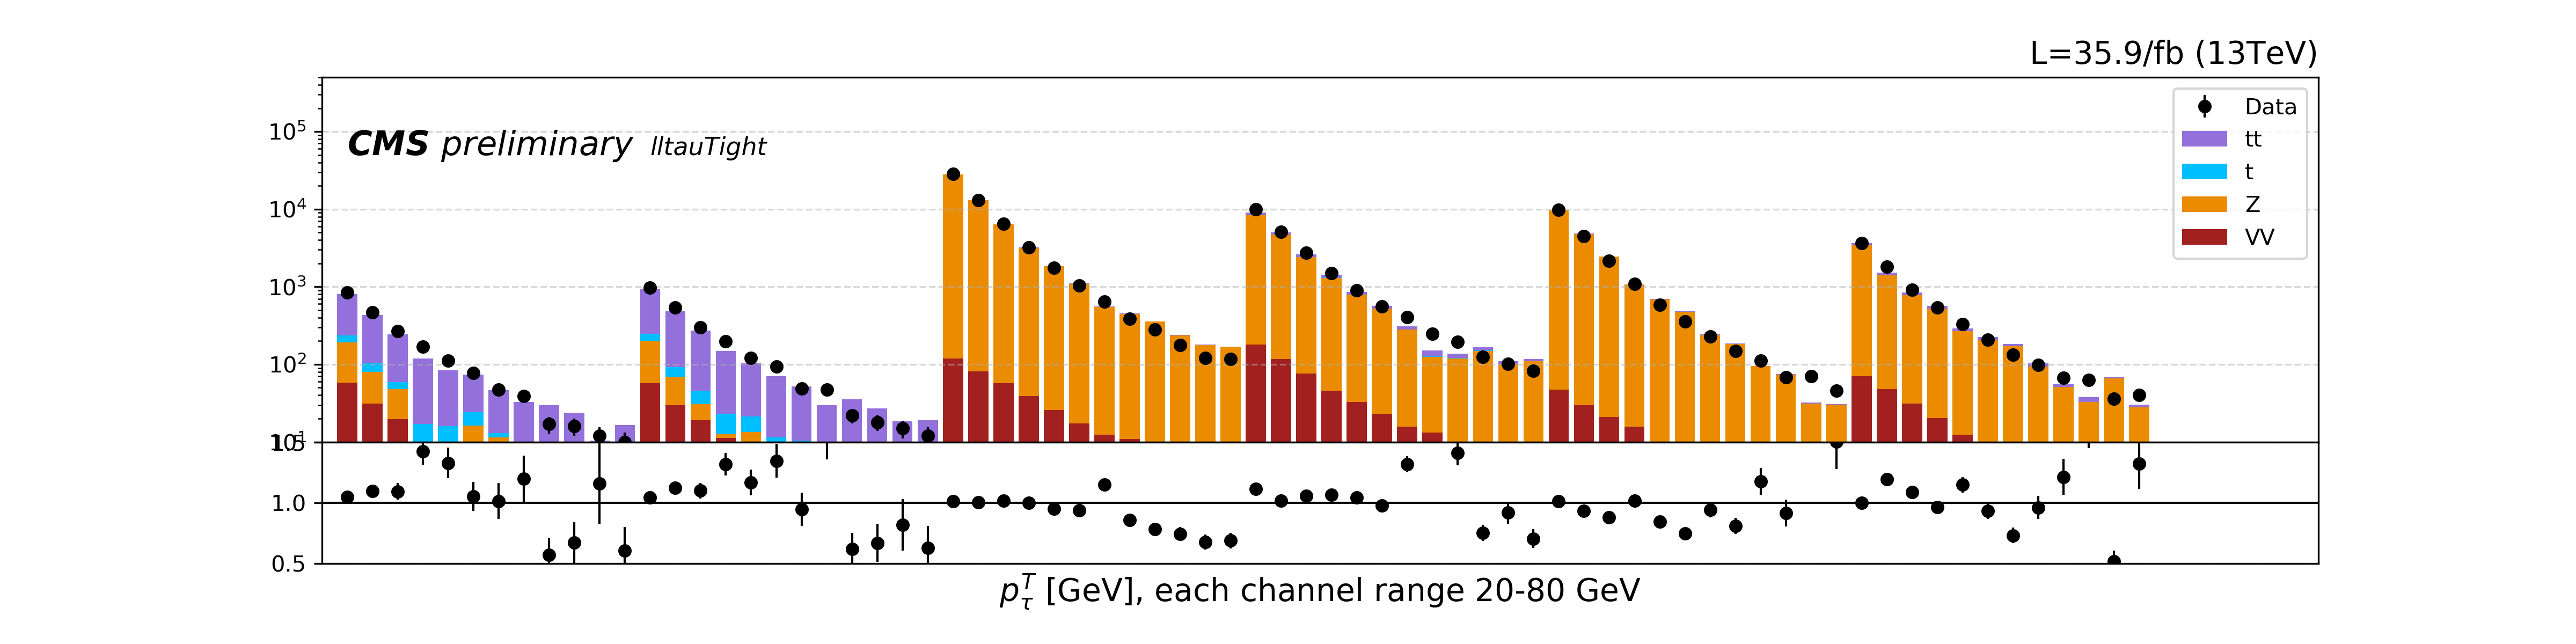
\includegraphics[width=0.99\textwidth]{chapters/Analysis/sectionCalibration/figures/jetToTauh/2020_tauID_prefit_lltauTight.png}
    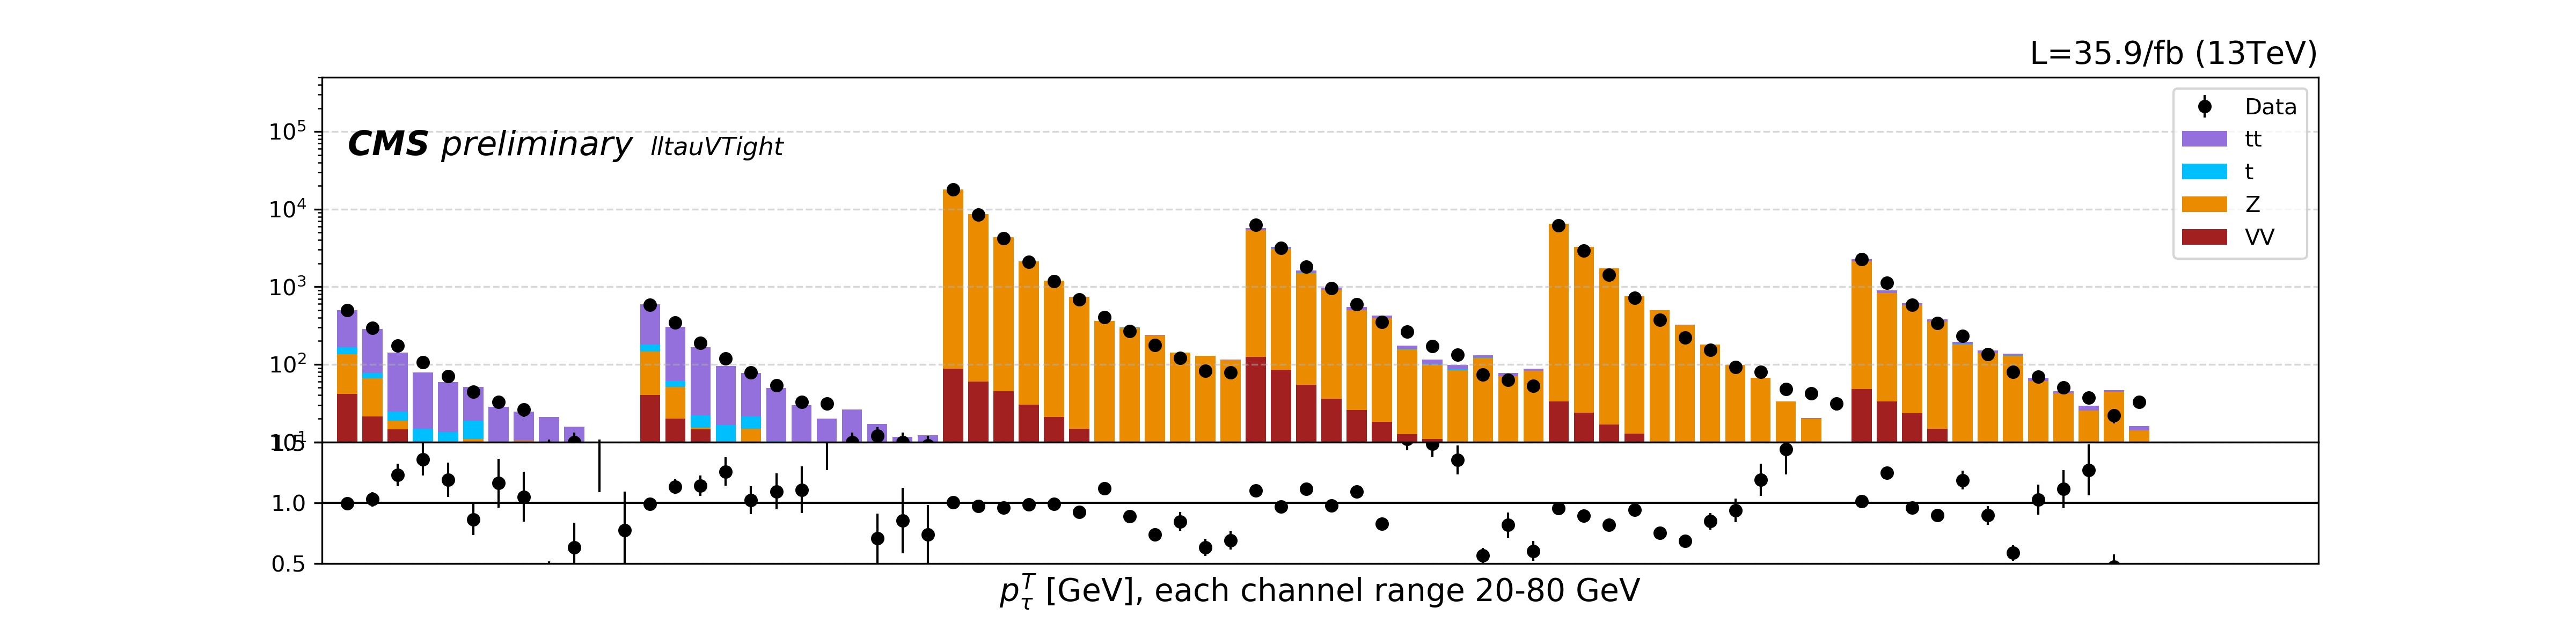
\includegraphics[width=0.99\textwidth]{chapters/Analysis/sectionCalibration/figures/jetToTauh/2020_tauID_prefit_lltauVTight.png}
    \caption{Prefit distributions of $\tau_h$ \pt. Upper and lower are the Tight and VTight WP.}
    \label{fig:appendix:fakeTauId:prefit}
\end{figure}

% \begin{figure}
%     \centering
%     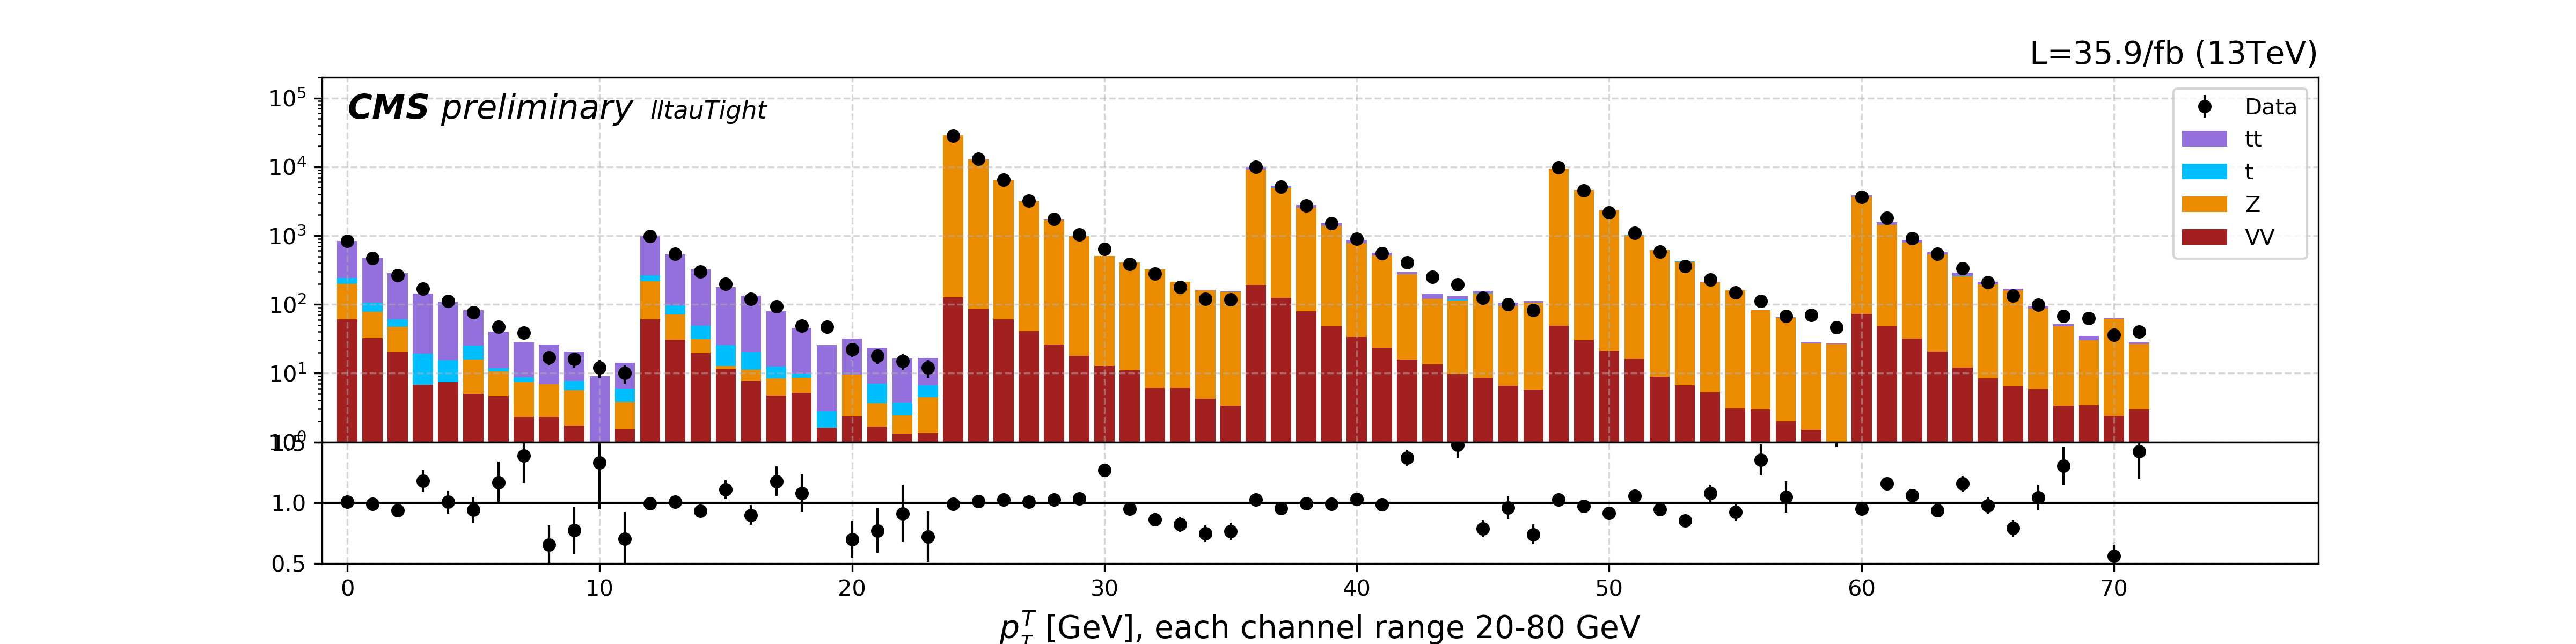
\includegraphics[width=0.99\textwidth]{chapters/Analysis/sectionCalibration/figures/jetToTauh/2020_tauID_postfit_lltauTight.png}
%     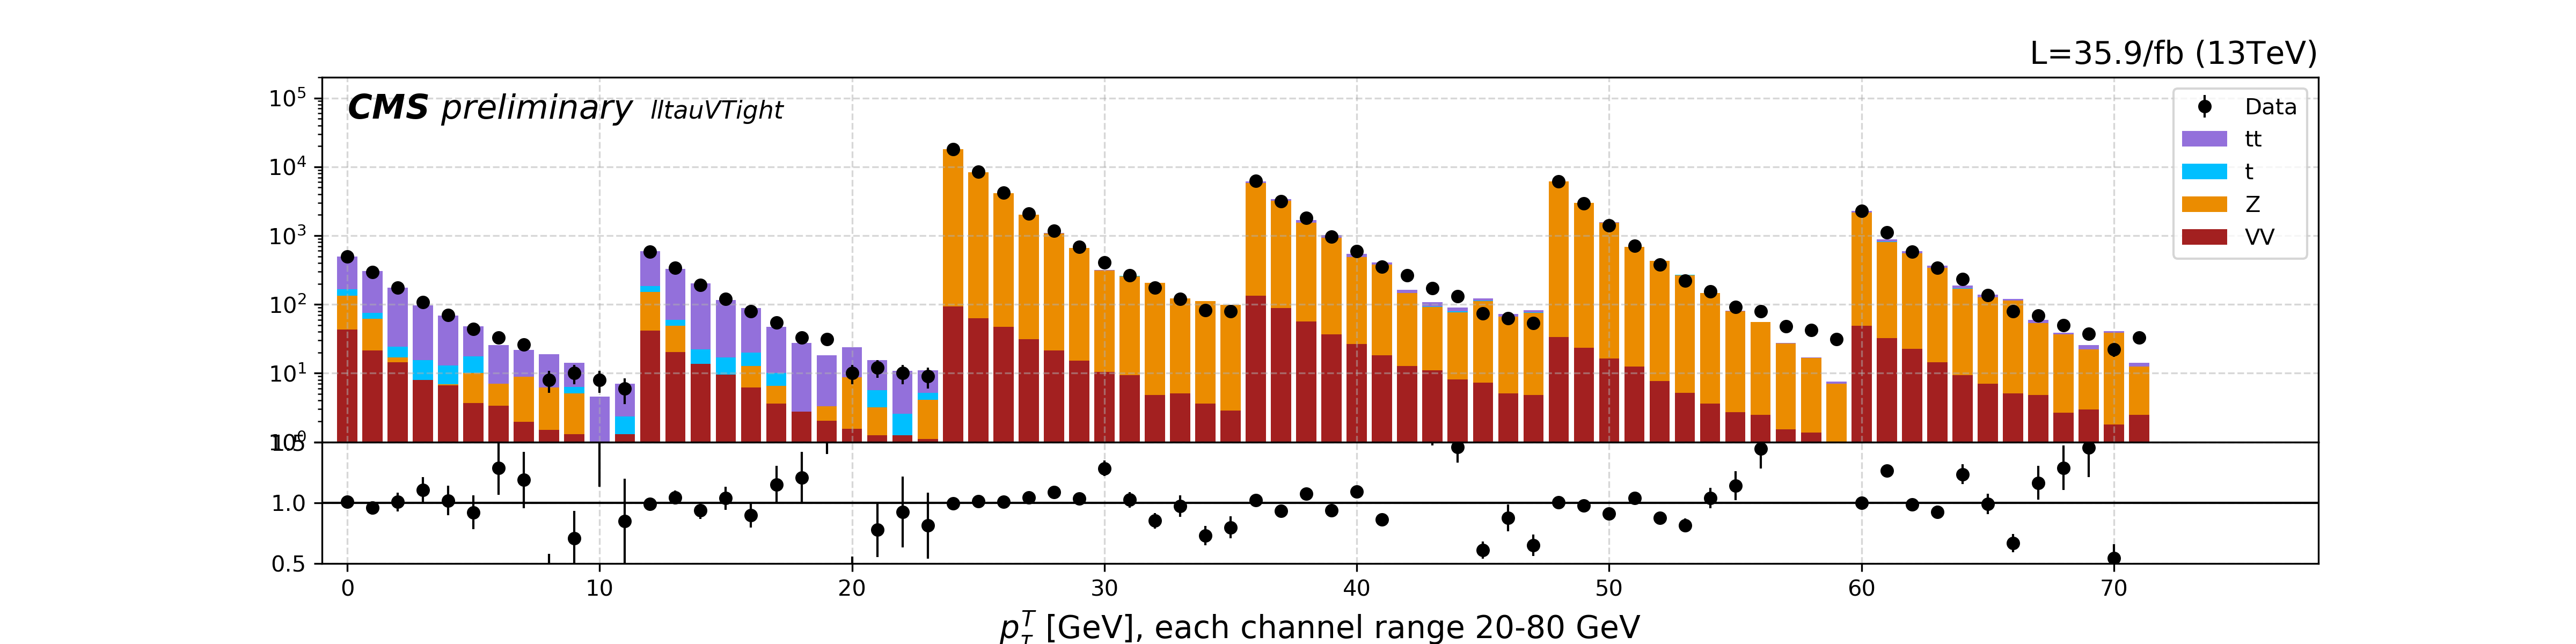
\includegraphics[width=0.99\textwidth]{chapters/Analysis/sectionCalibration/figures/jetToTauh/2020_tauID_postfit_lltauVTight.png}
%     \caption{Post distributions of $\tau_h$ \pt. Upper and lower are the Tight and VTight WP. }
%     \label{fig:appendix:fakeTauId:postfit}
% \end{figure}




To measure $SF (q\to \tau_h)$  and $SF (b\to \tau_h)$, a template fit to the $\tau_h$ \pt is performed.   The free parameters are $SF (q\to \tau_h)$  and $SF (b\to \tau_h)$ in 5 \pt bins from 20-80 GeV.  The systematical uncertainties, including cross sections, luminosity, electron/muon efficiency, are taken into account as nuisance parameters in the fit.



% \subsection{Result of the Scale Factors}



\begin{figure}
    \centering
    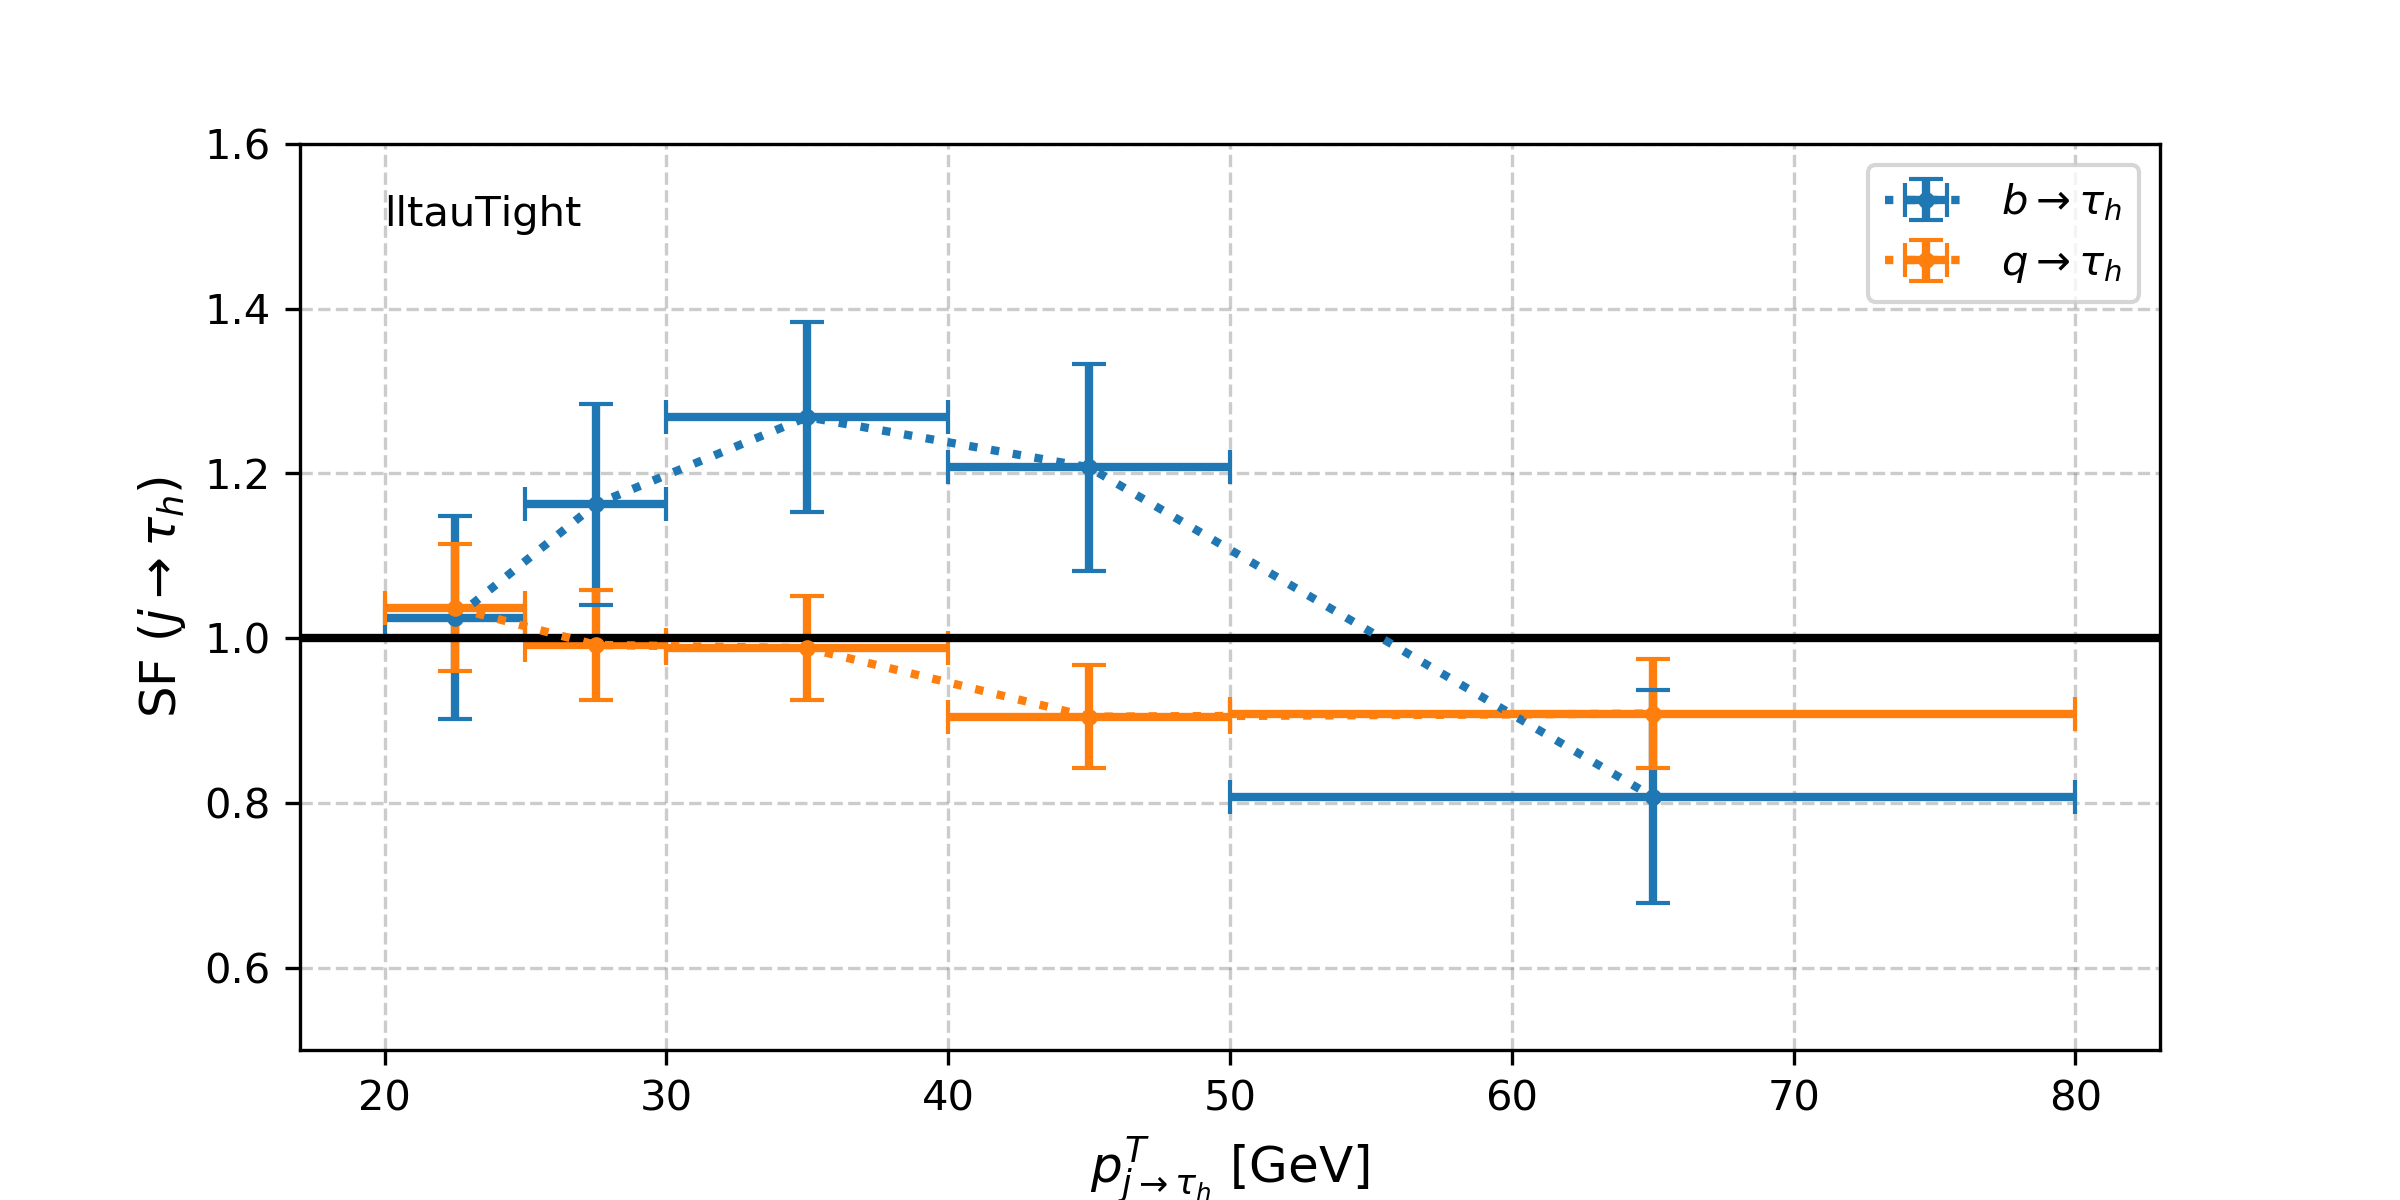
\includegraphics[width=0.49\textwidth]{chapters/Analysis/sectionCalibration/figures/jetToTauh/fit2_ptflavor2_lltauTight.png}
    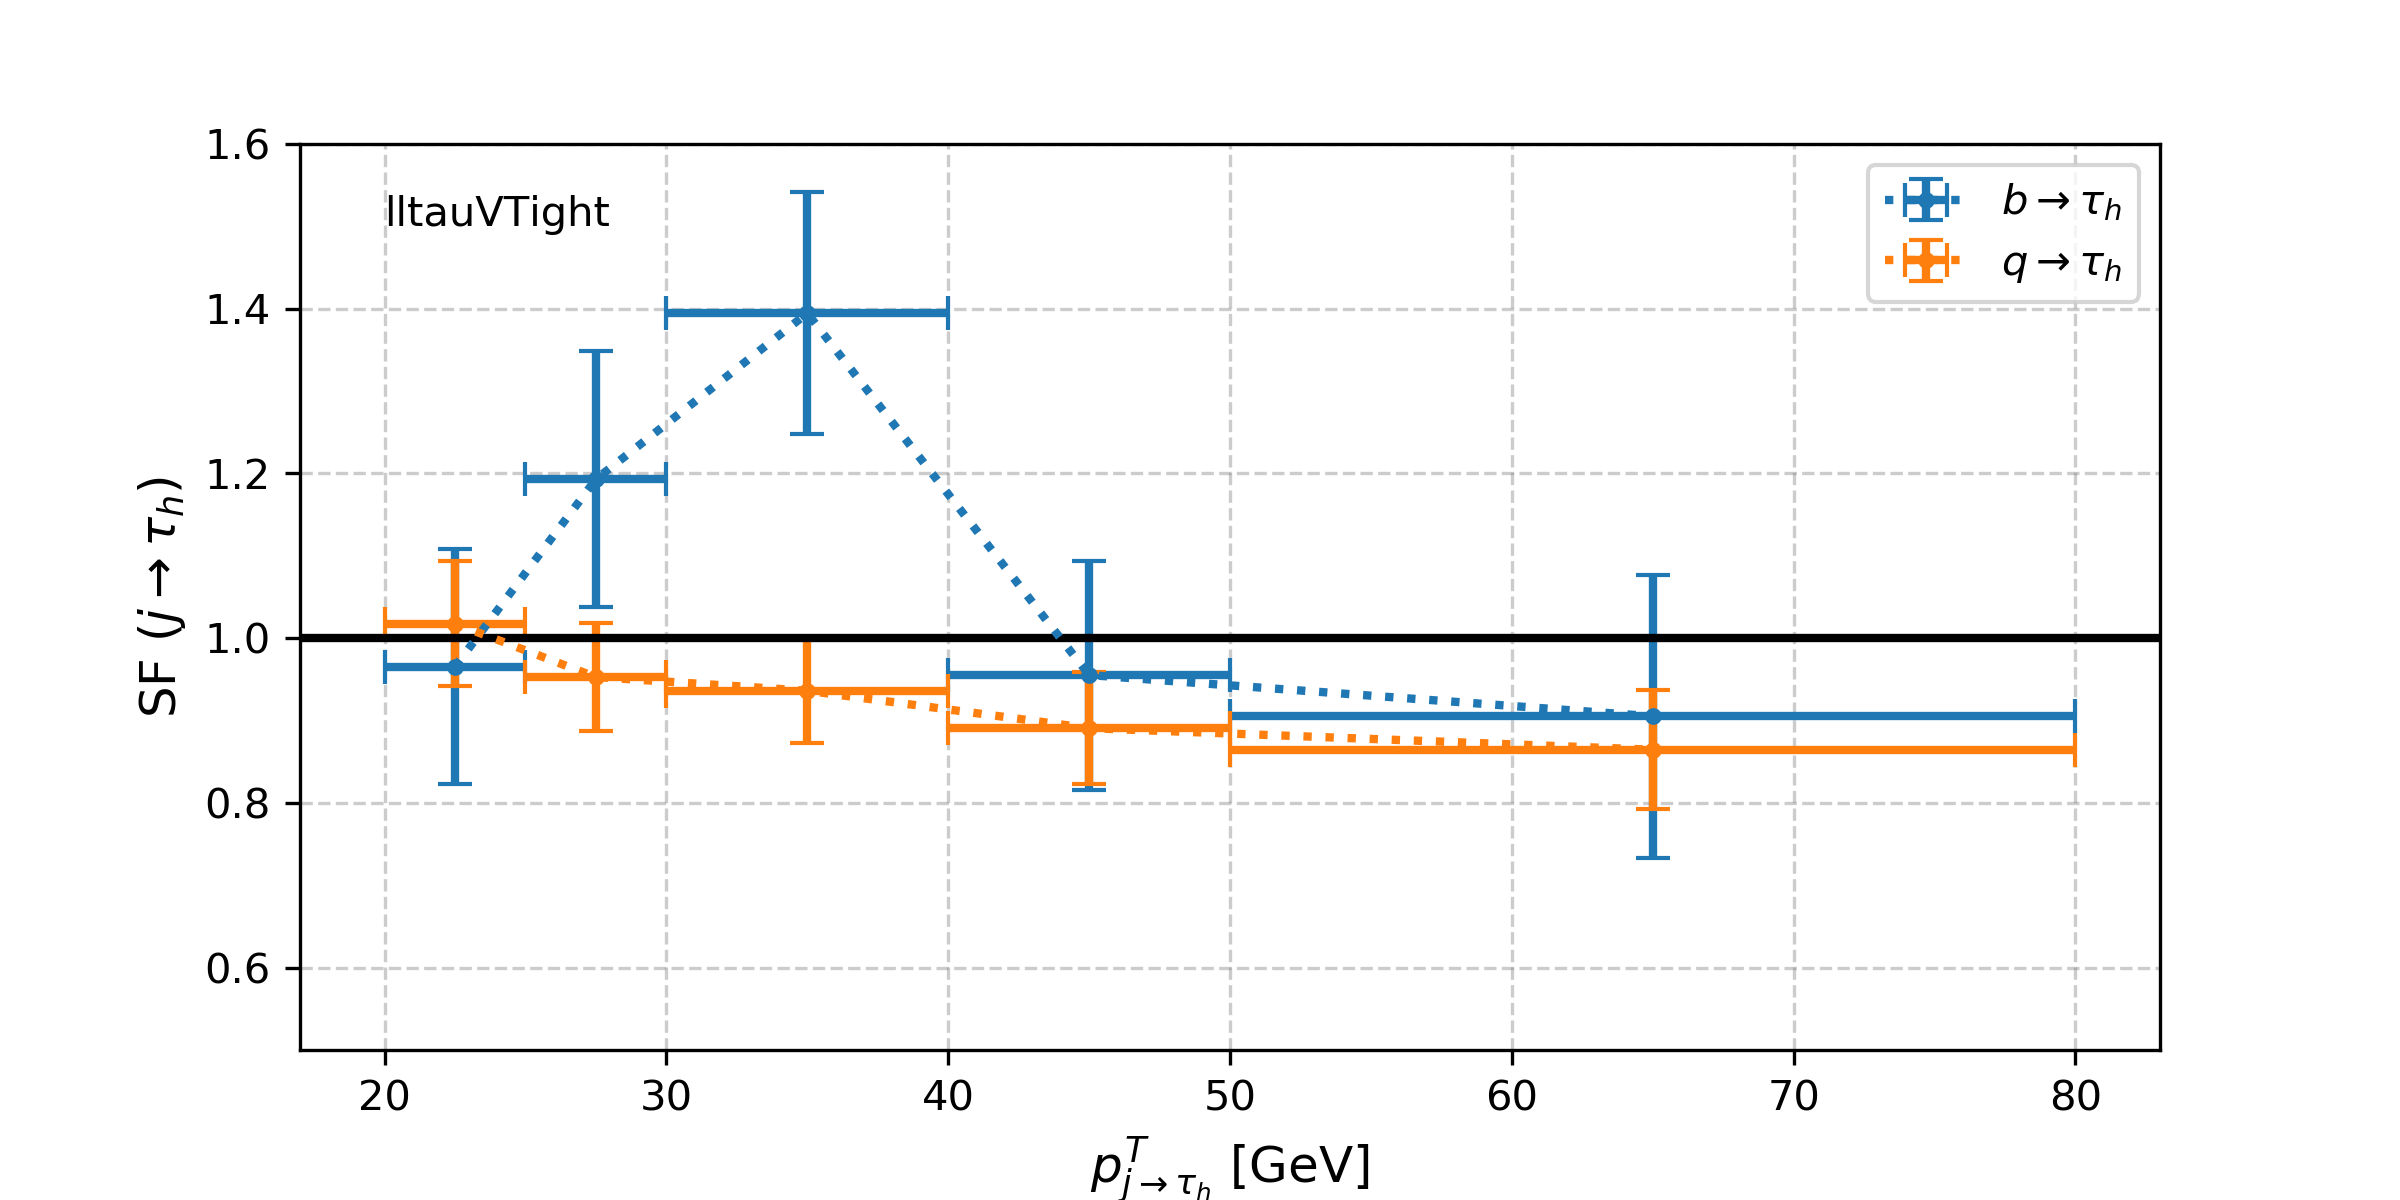
\includegraphics[width=0.49\textwidth]{chapters/Analysis/sectionCalibration/figures/jetToTauh/fit2_ptflavor2_lltauVTight.png}
    \caption{$SF (j\to \tau_h)$ for Tight and VTight tau.}
    \label{fig:appendix:fakeTauId:fit}
\end{figure}



The result of $SF (j\to \tau_h)$ for Tight and VTight WP are shown in figure~\ref{fig:appendix:fakeTauId:fit} and table~\ref{tab:appendix:fakeTauId:fit} The pulls and correlation matrix of the template fit are shown in Figure~\ref{fig:appendix:fakeTauId:fitparam}

In shape analysis, the uncertainty of $SF (j \to \tau_h)$ will be used as prefit uncertainty of the corresponding nuisance parameters.  In counting analysis,  the measured $SF (j \to \tau_h)$ will be variate according to the measured uncertainties.




\begin{figure}
    \centering
    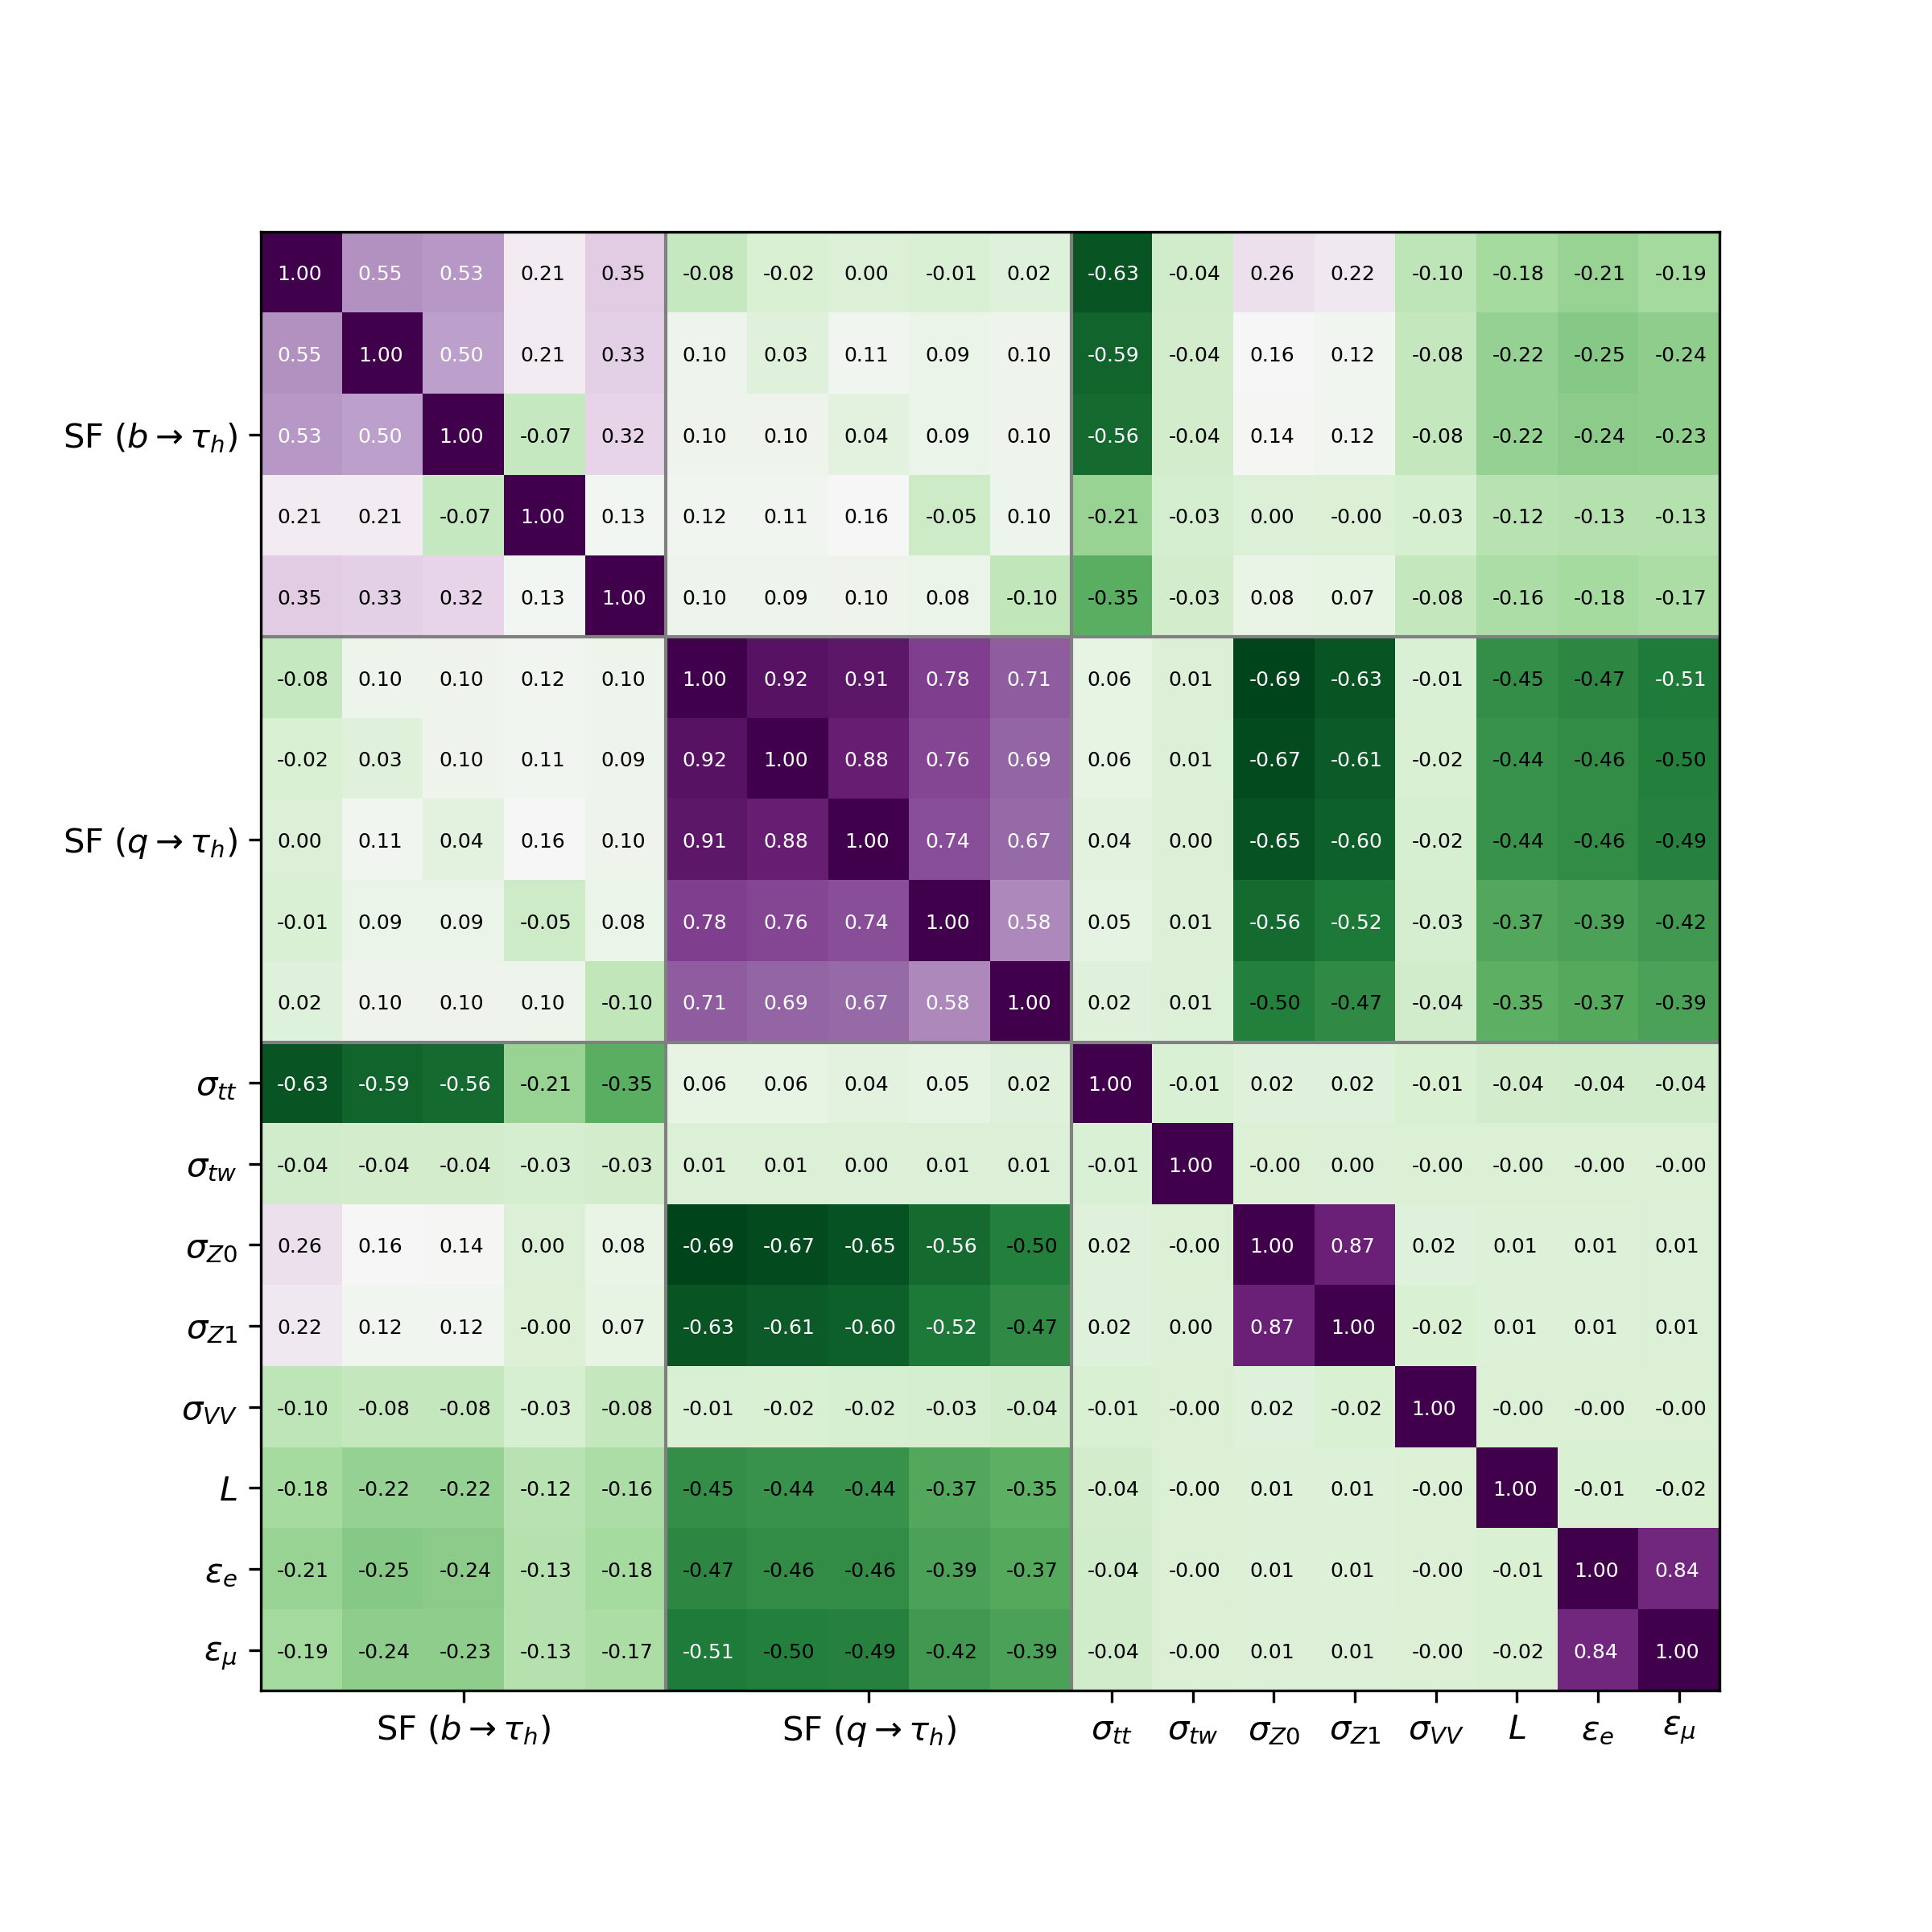
\includegraphics[width=0.49\textwidth]{chapters/Analysis/sectionCalibration/figures/jetToTauh/corr2_lltauTight_splitJetFlavor.png}
    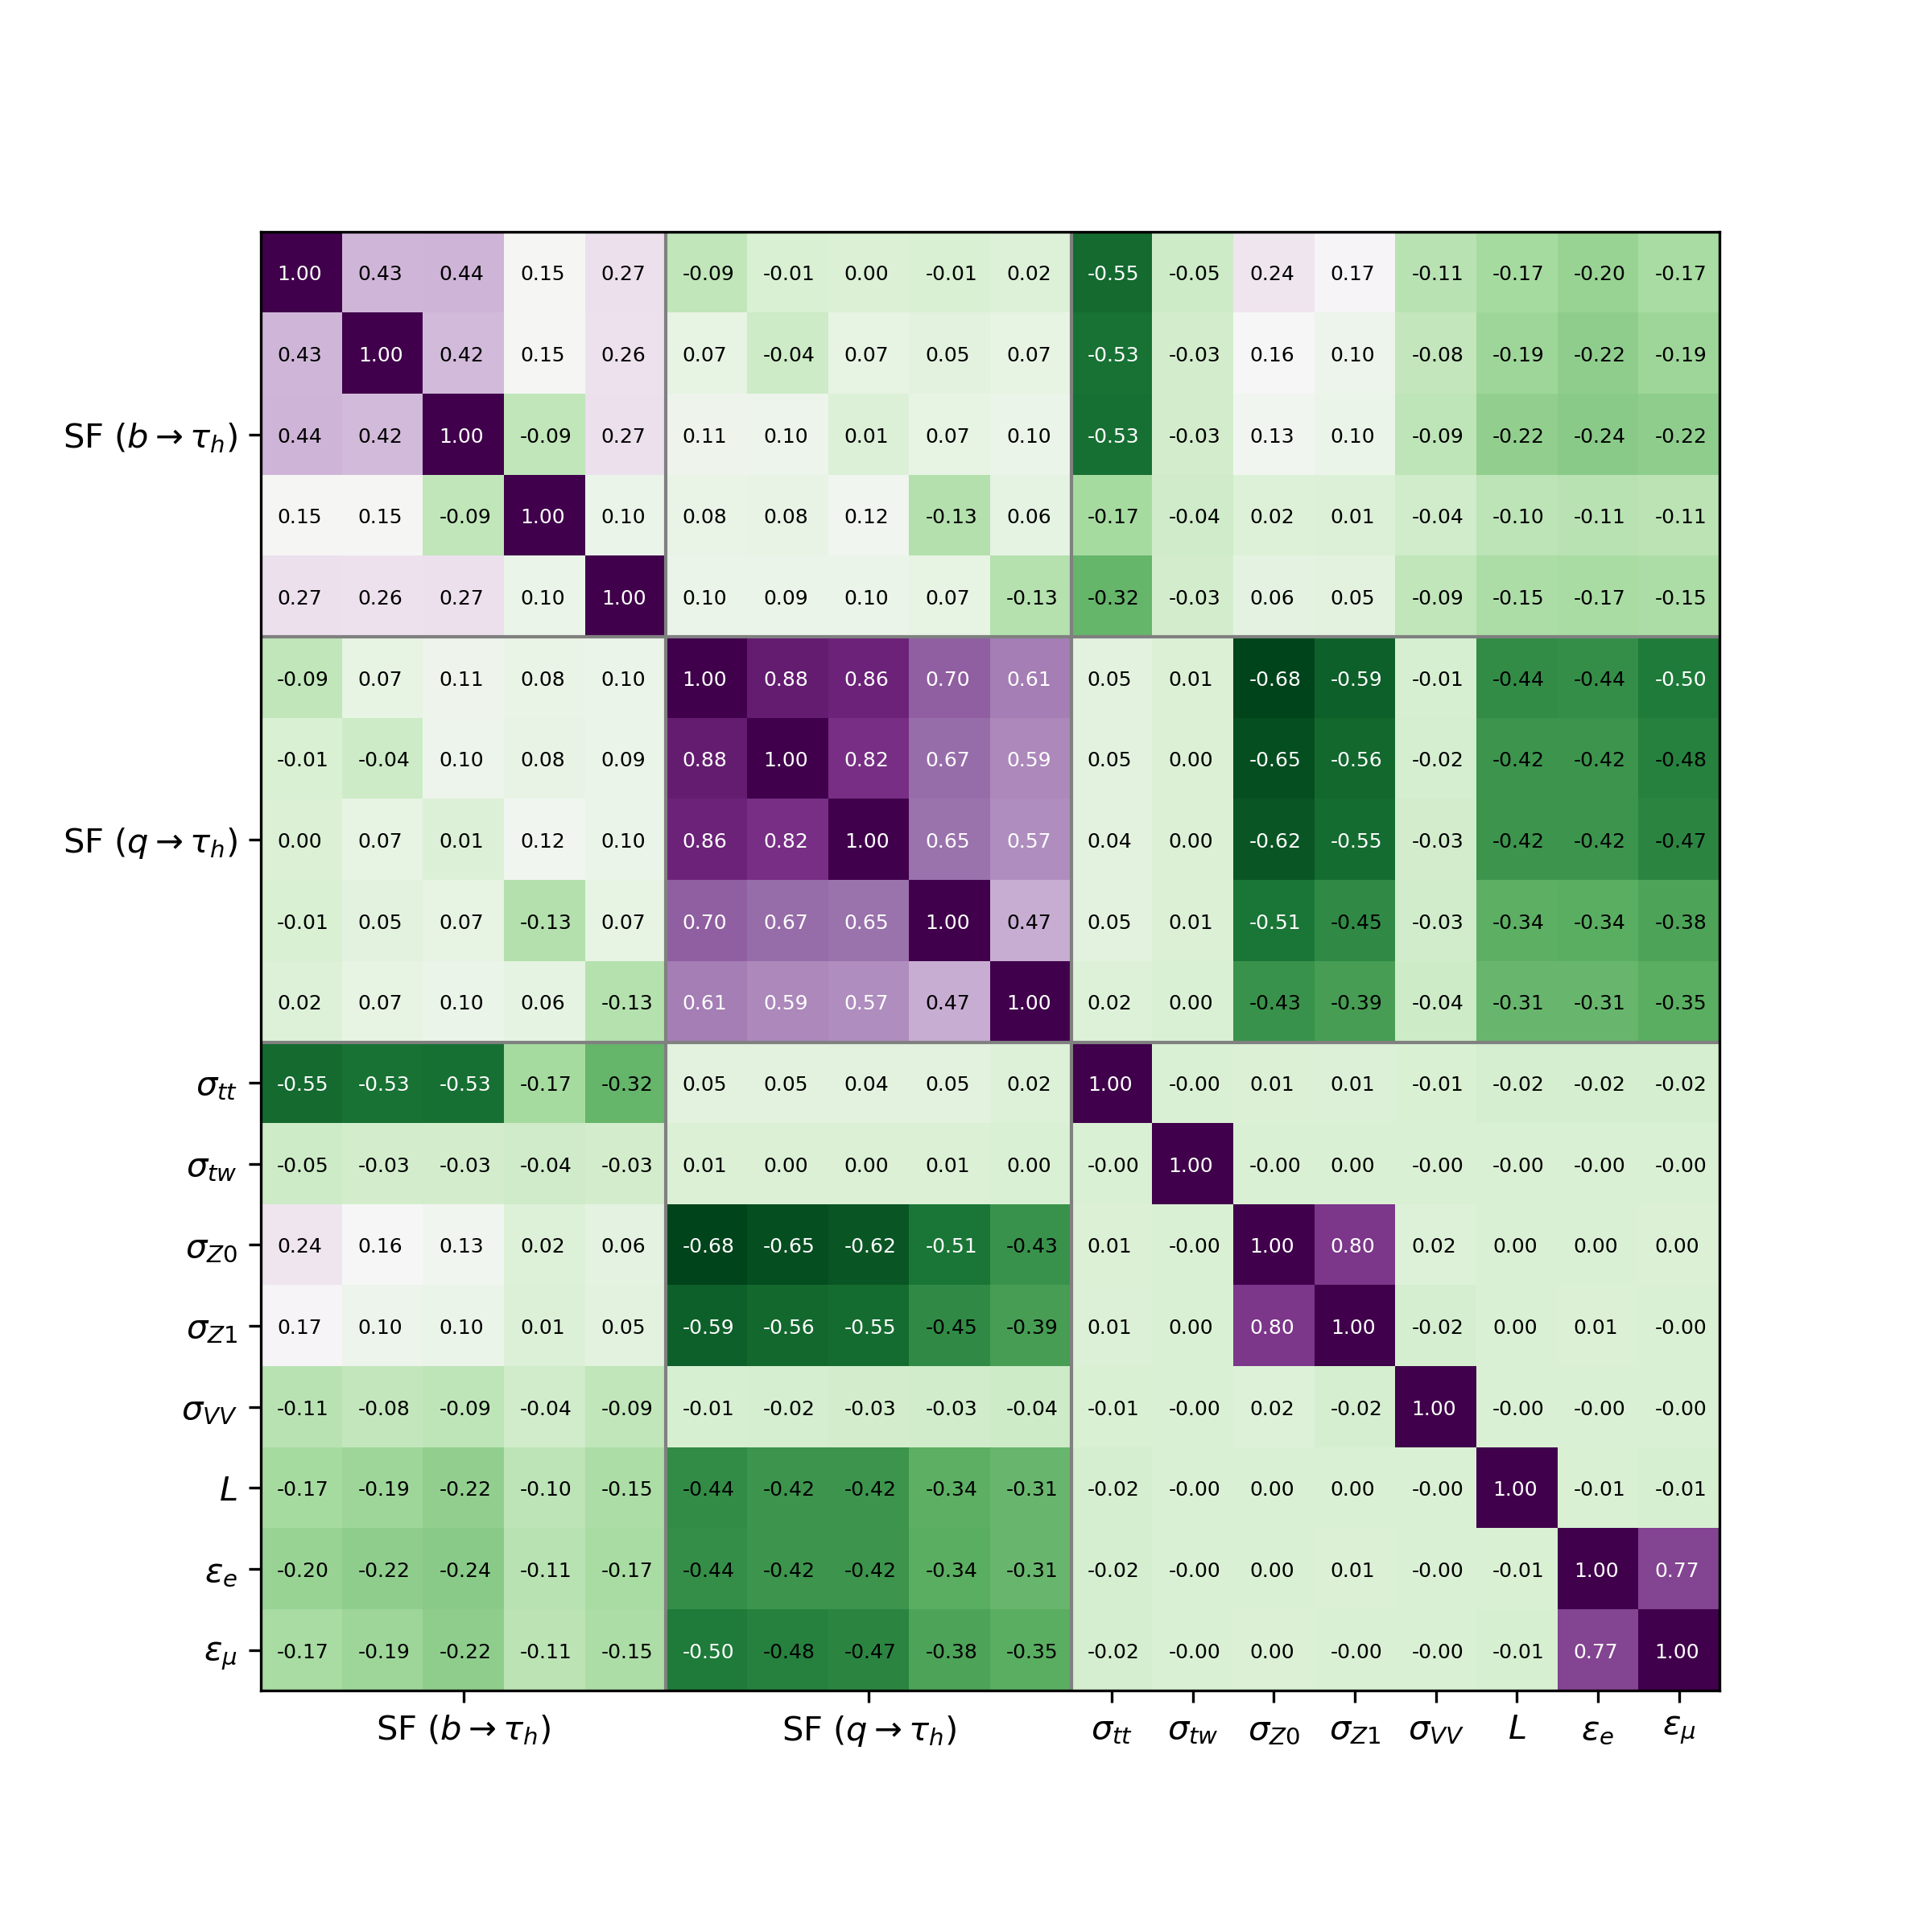
\includegraphics[width=0.49\textwidth]{chapters/Analysis/sectionCalibration/figures/jetToTauh/corr2_lltauVTight_splitJetFlavor.png}
    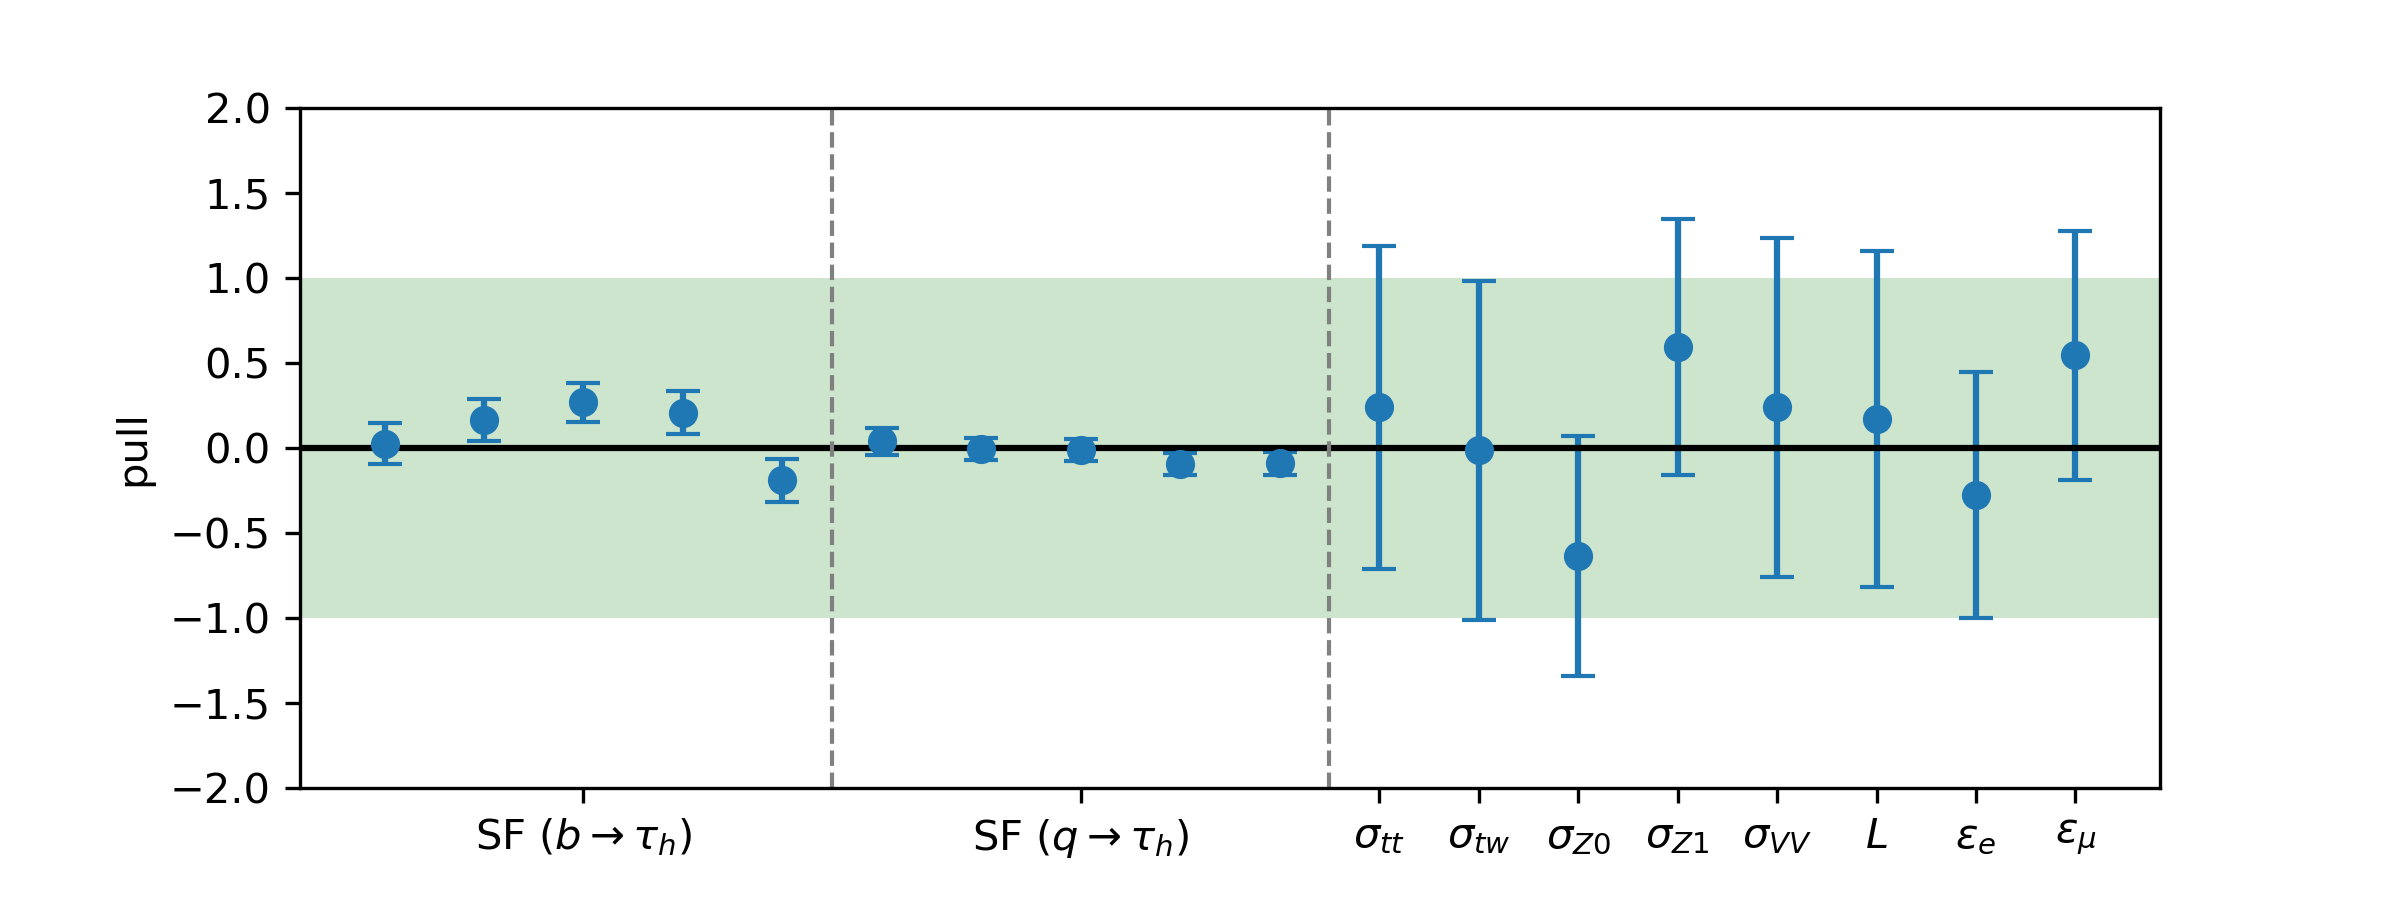
\includegraphics[width=0.49\textwidth]{chapters/Analysis/sectionCalibration/figures/jetToTauh/pull2_lltauTight_splitJetFlavor.png}
    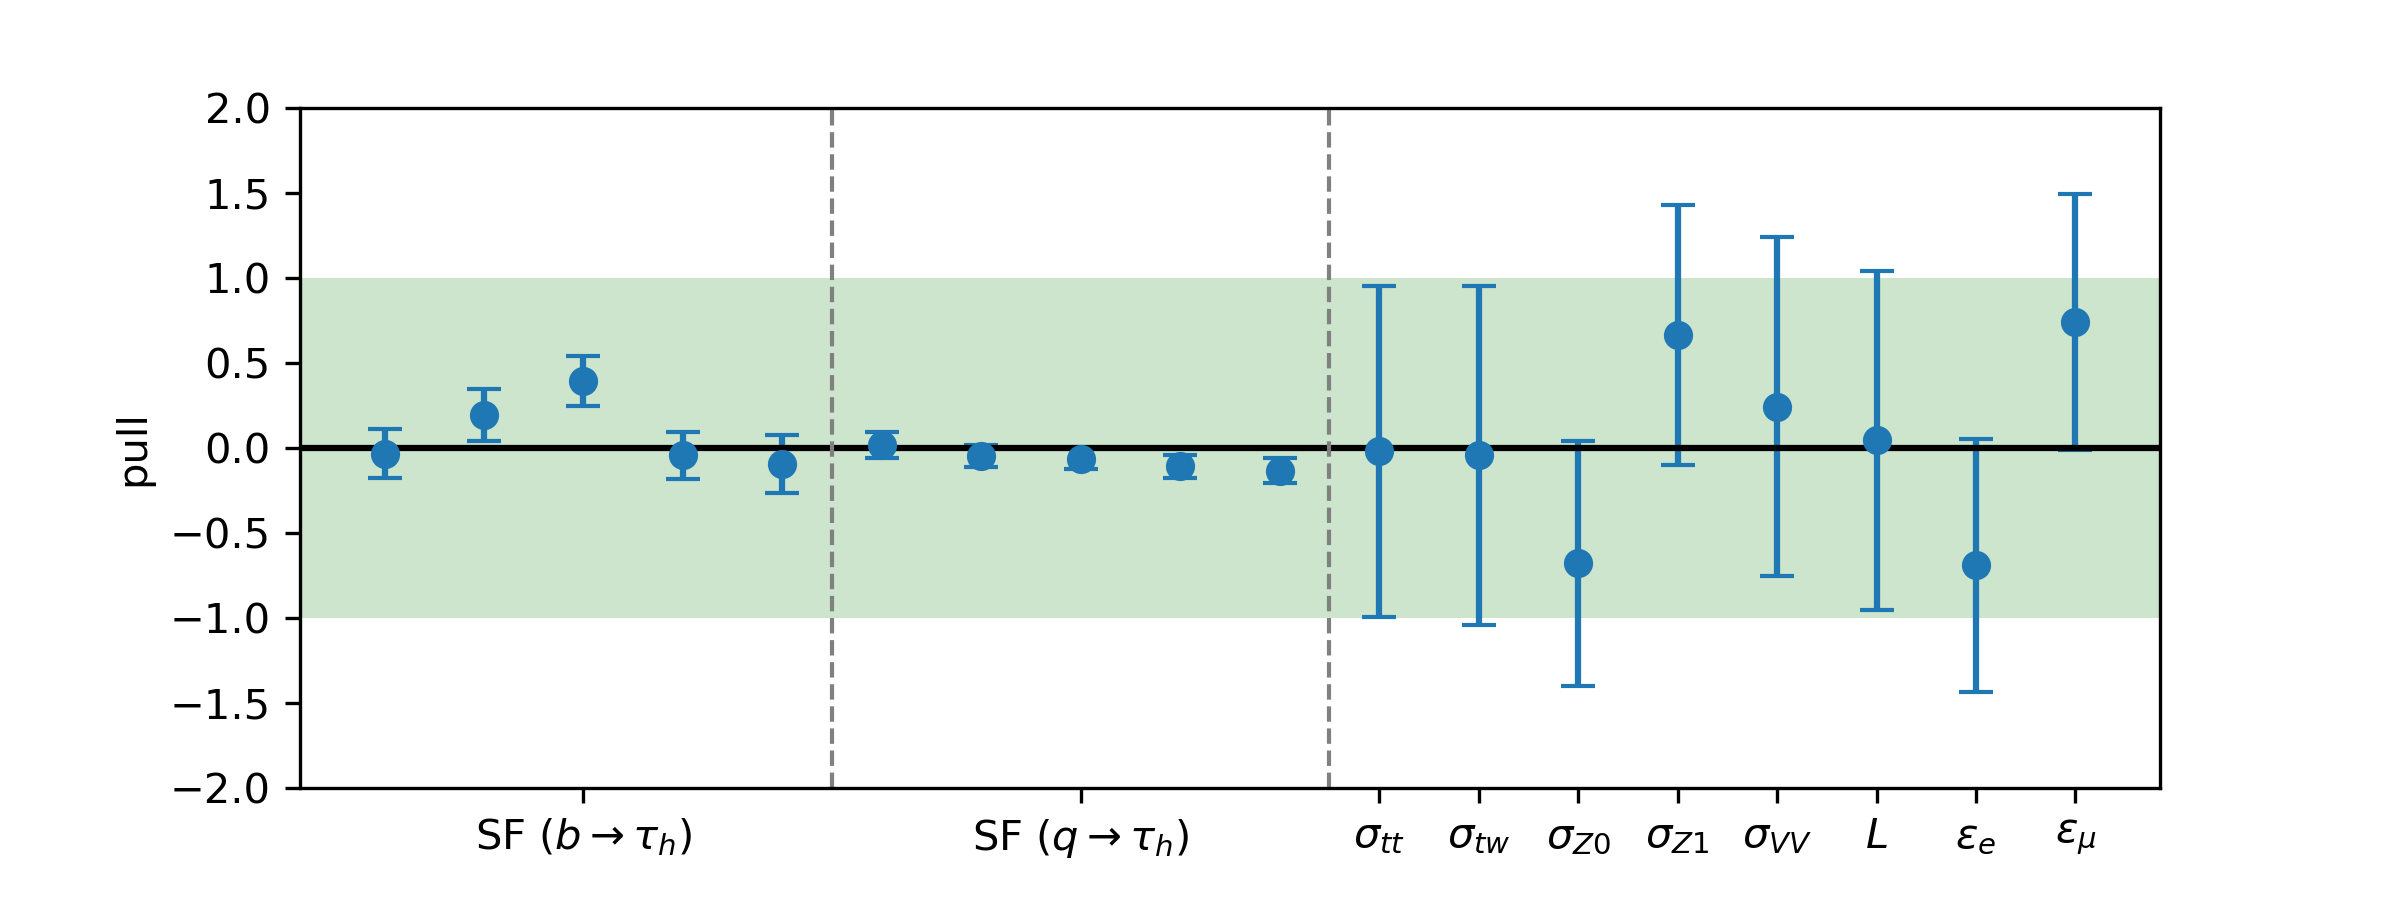
\includegraphics[width=0.49\textwidth]{chapters/Analysis/sectionCalibration/figures/jetToTauh/pull2_lltauVTight_splitJetFlavor.png}
    \caption{The correlation matrix and the pulls of the fitting parameters for Tight (left) and VTight (right) $\tau_h$. }
    \label{fig:appendix:fakeTauId:fitparam}
\end{figure}



\begin{table}[h]
    \setlength{\tabcolsep}{6pt} % Default value: 6pt
    \renewcommand{\arraystretch}{1.5} % Default value: 1
    \caption{ $SF (j\to \tau_h)$ for Tight and VTight tau.}
    
    \begin{tabular}{c|ccccc}
    \hline
    $p^T_{\tau_h}$ [GeV]  & 20-25         & 25-30         & 30-40         & 40-50         & 50-80         \\
    \hline
    $SF(b\to \rm{Tight} \; \tau_h)$  & $1.02\pm0.12$ & $1.16\pm0.12$ & $1.27\pm0.11$ & $1.21\pm0.13$ & $0.81\pm0.13$ \\
    $SF(q\to \rm{Tight} \;  \tau_h)$  & $1.04\pm0.08$ & $0.99\pm0.07$ & $0.99\pm0.06$ & $0.90\pm0.06$ & $0.91\pm0.07$ \\
    \hline
    $SF(b\to \rm{VTight} \; \tau_h)$ & $0.97\pm0.14$ & $1.19\pm0.16$ & $1.39\pm0.15$ & $0.96\pm0.14$ & $0.91\pm0.17$ \\
    $SF(q\to \rm{VTight} \; \tau_h)$ & $1.02\pm0.08$ & $0.95\pm0.07$ & $0.94\pm0.06$ & $0.89\pm0.07$ & $0.86\pm0.07$ \\
    \hline
    \end{tabular}
 
    \label{tab:appendix:fakeTauId:fit}
\end{table}


\FloatBarrier




\subsection{Measurement of b-tag Efficiencies in Simulation}
\label{sec:analysis:calibration:btag}


% \subsection{Corrections for b-tag Efficiencies}


To account for differences of the b-tag efficiency in data and simulation, a method that modifies the b-tag status of a jet is adopted in the simulation. In the method, the status is modified based on a set of data-to-simulation scale factors derived by the b-tag POG, and the efficiencies for simulation which have been measured independently in this section.  The method of the b-tag correction for simulation works as follows:

\begin{itemize}

    \item jets are identified as originating from the decay of a b quark, c quark, or ``light" parton (usdg) from generator truth information. Depending on the parton flavor and jet \pt, the appropriate scale factor $f_{\epsilon}$ and efficiency from simulation $\epsilon$ are looked up from a map.
    
    \item if $f_{\epsilon} < 1$, then a b-tagged jet is downgraded to a non-b tagged jet with probability,
        \begin{equation}
            p = 1 - f_{\epsilon}.
        \end{equation}
        \noindent if it is not b-tagged, nothing is changed.
    
    
    \item if $f_{\epsilon} > 1$, then a non-b-tagged jet is upgraded to a b-tagged jet with probability,
        \begin{equation}
            p = \frac{1 - f_{\epsilon}}{1 - \frac{1}{\epsilon}}.
        \end{equation}
        \noindent If it is already b-tagged, its status is unchanged.
\end{itemize}

% \subsection{b-tag Efficiencies in the Simulation}

Measurement of the b-tag efficiency in simulation relies on knowing the flavor of the parton that gives rise to the jet.  This is done with official CMS tools that assign a jet flavor based on the characteristics of the quark and gluon content of a jet~\cite{twiki:jet_mc_flavor}.  The efficiencies are measured for the case of b, c, and light (usdg) flavor jets, and as a function of the jet \pt.  That is,
\begin{equation}
    \epsilon(\pt, \mathrm{flavor}) = \frac{ N_{\mathrm{pass}}(\pt, \mathrm{flavor})} {N(\pt, \mathrm{flavor})},
\end{equation}

\noindent where the numerator is the number of jets passing the b-tag working point, and the denominator is the total number of jets considered. These quantities are measured in both \ttbar and \PZ plus jet samples. The CSVv2 discriminator value for the two samples are shown in figures~\ref{fig:btag_csvv2} for the three jet flavor categories. The efficiency measurement uses the middle working point of CSVv2 discriminator, the same as the selection in the measurement of \PW branching fraction. The result of b-tagging efficiencies is shown in figure~\ref{fig:btag_eff}.  There is some level of disagreement between the two samples for the b quark jets that likely could be attributed to the \ttbar sample being generated with an NLO generator (\POWHEG) and the \PZ plus jet sample being generated with a LO generator (\MADGRAPH). The efficiencies from \ttbar sample is used for the b-tag correction. The events used for the selection require at least muon passing our analysis requirements, and the four leading \pt jets are considered in the measurement.

\begin{figure}[h!]
    \centering
    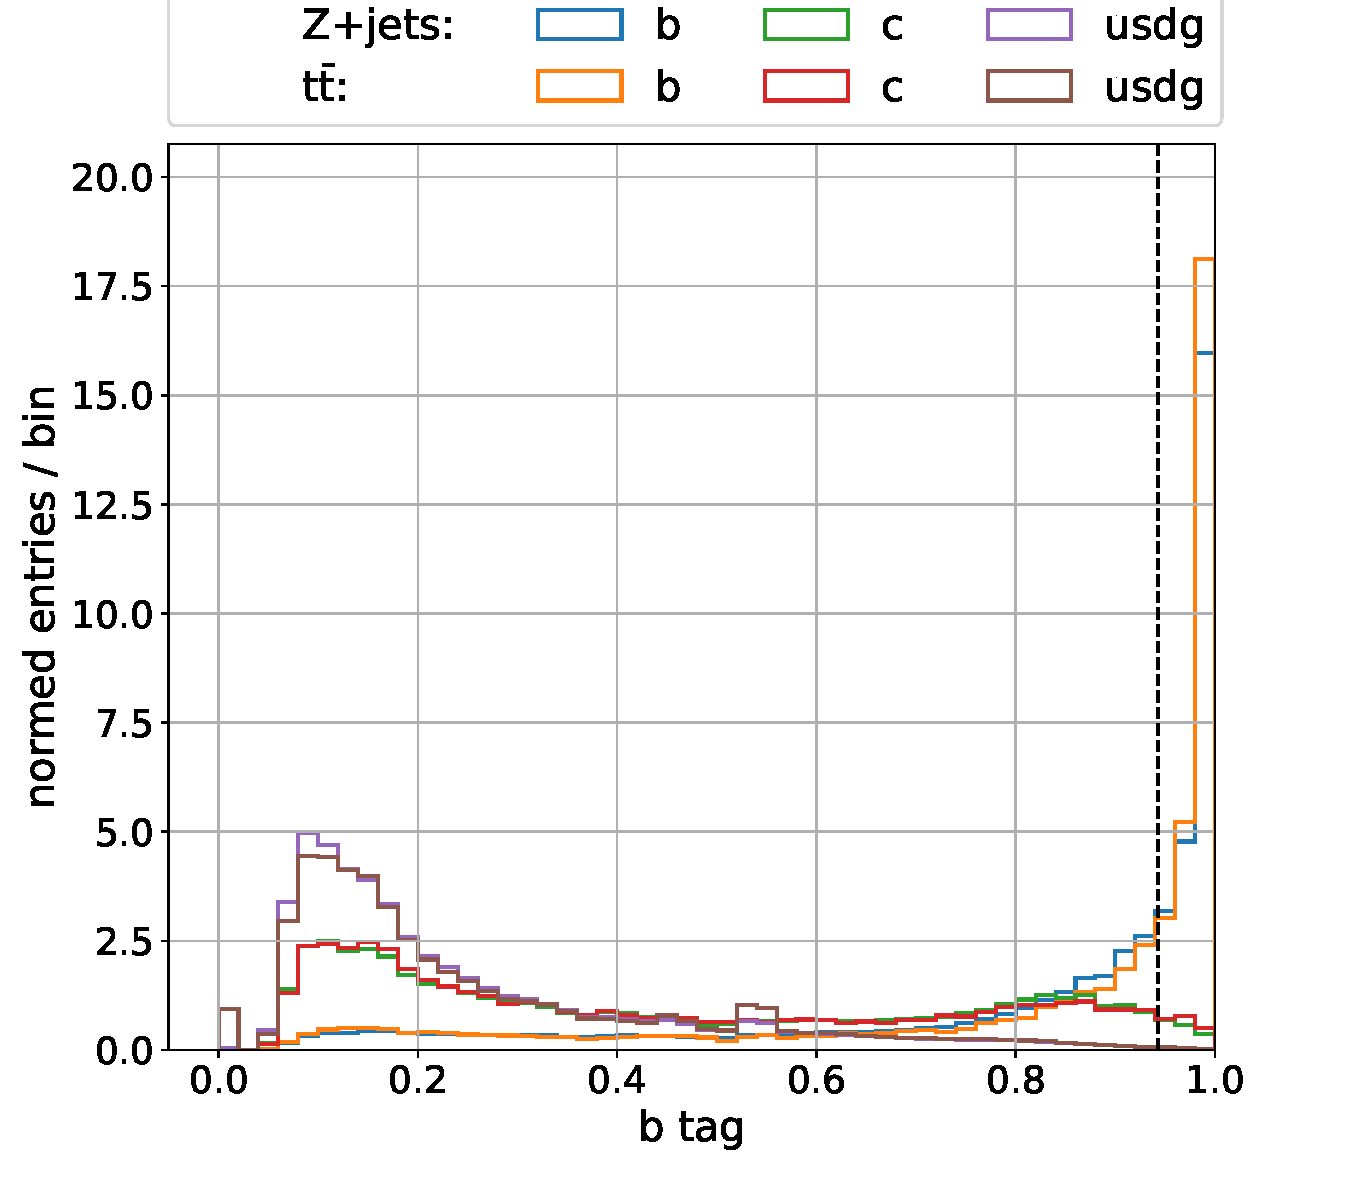
\includegraphics[width=0.45\textwidth]{chapters/Analysis/sectionCalibration/figures/btag/bmva_mc.pdf}
    \caption{Distribution of ``csv" b-tag discriminator for the three flavor categories under consideration for \PZ + jet and \ttbar events.      
    \label{fig:btag_csvv2}}
\end{figure}

\begin{figure}[h!]
    \centering
    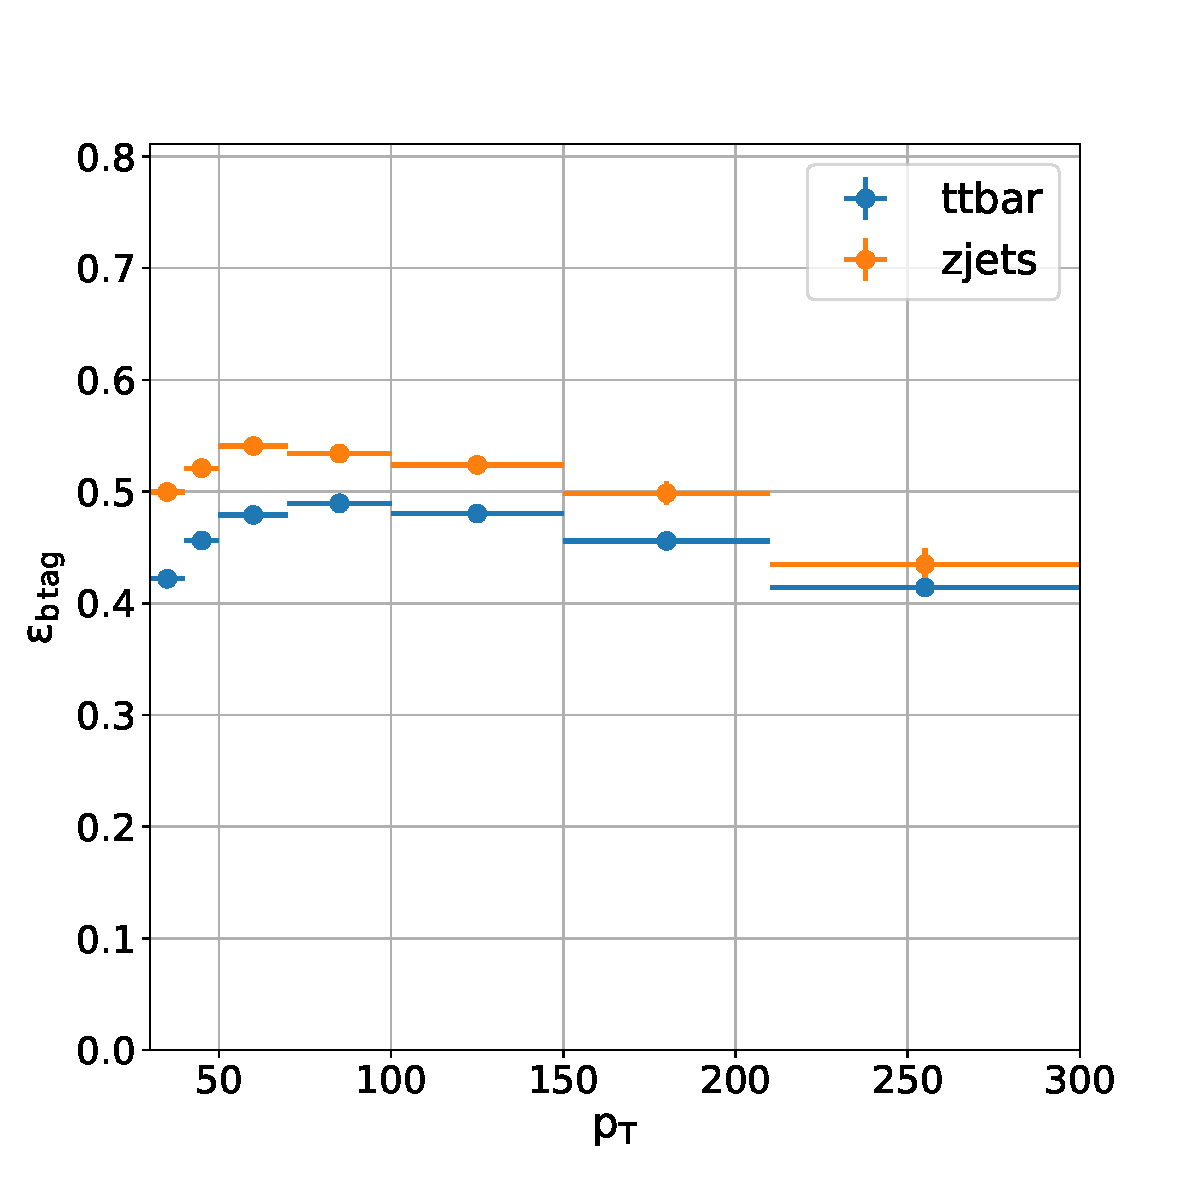
\includegraphics[width=0.3\textwidth]{chapters/Analysis/sectionCalibration/figures/btag/bmva_mceff_vs_pt_b}
    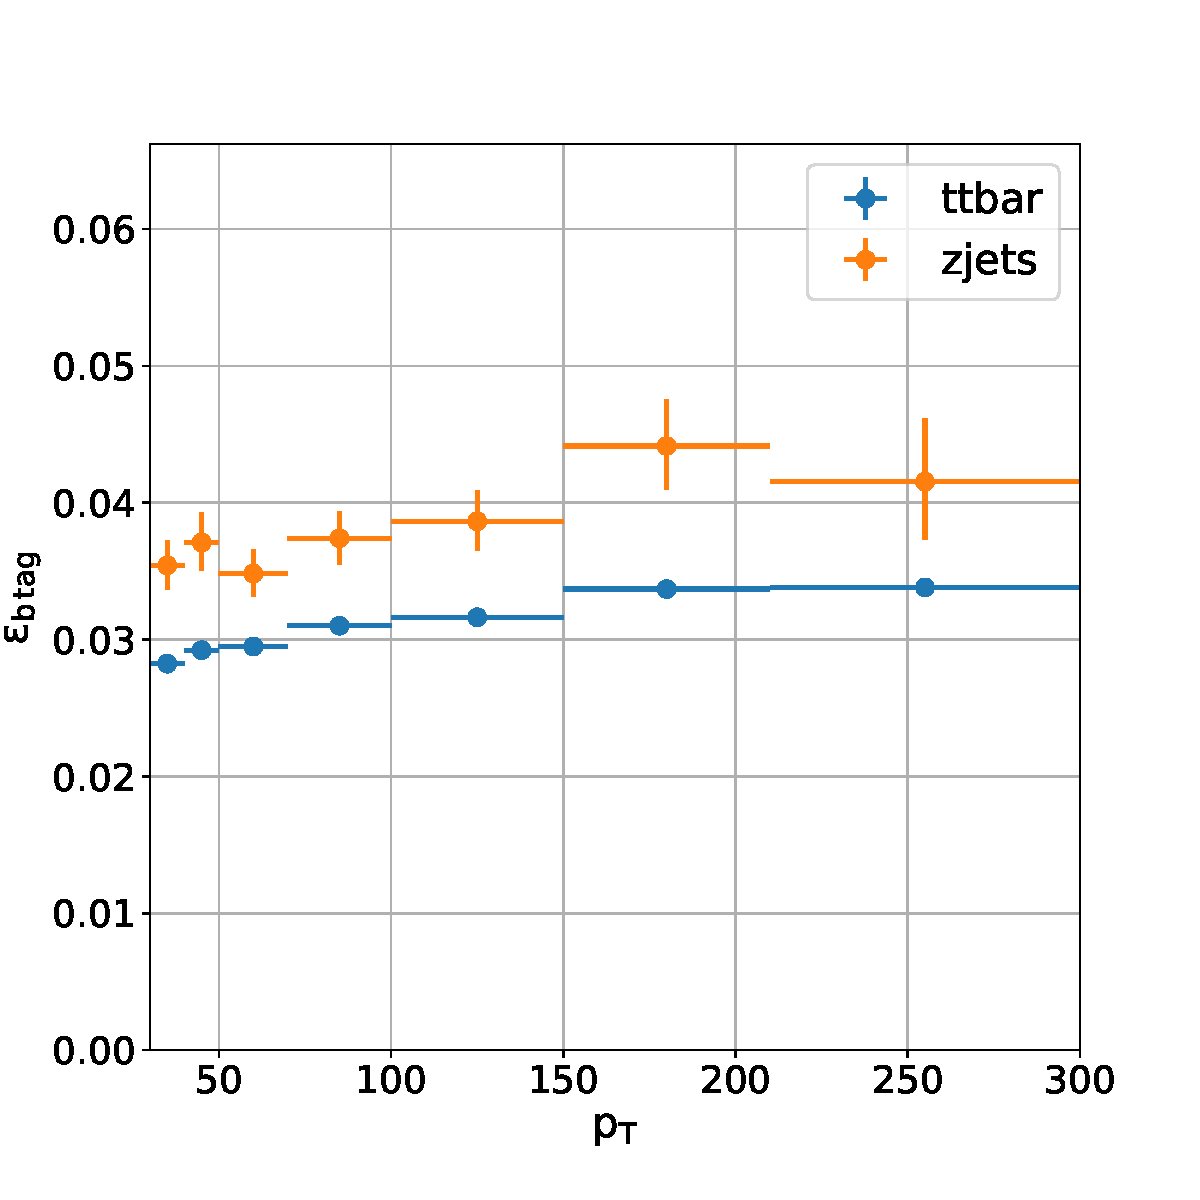
\includegraphics[width=0.3\textwidth]{chapters/Analysis/sectionCalibration/figures/btag/bmva_mceff_vs_pt_c}
    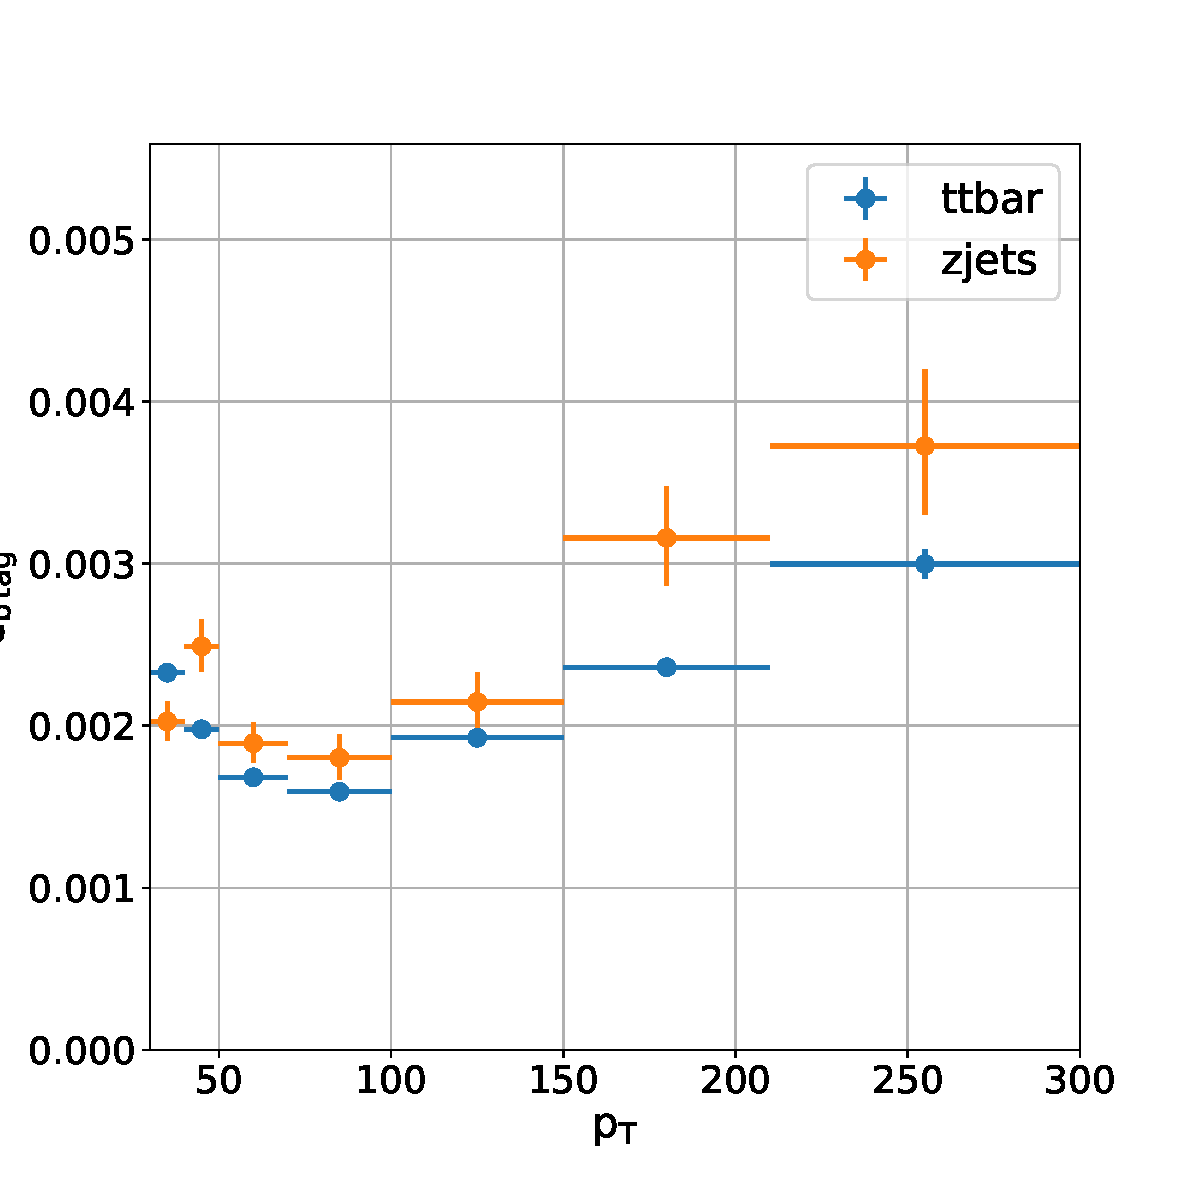
\includegraphics[width=0.3\textwidth]{chapters/Analysis/sectionCalibration/figures/btag/bmva_mceff_vs_pt_usdg}
    \caption{Efficiency to b-tag a jet originating from a b quark (left), c quark (middle), and light quark (right).
    \label{fig:btag_eff}
    }
\end{figure}

\FloatBarrier





\subsection{Reweight of Different Hadronic Tau Decay Modes in the Simulation}
\label{sec:analysis:calibration:tauBr}

The MC events with $\tau_h$ in the $e\tau$ and $\mu \tau$ channel is essential to the sensitivity of the $Br(W\to\tau)$ measurement. However, the tau's hadronic decay branching fraction $B(\tau \to  \rm{hadrons})$ in the MC simulation are different from the experimental world average in the PDG. The $\tau_h$ selection efficiency could be impacted by such difference because various tau's hadronic  decay mode have different efficiencies in the CMS $\tau_h$ reconstruction with SPH algorithm.

Thus it is necessary to reweight the MC events to correct the deviation of tau's decay in the simulation with respect to the PDG values. For the values in the \PYTHIA simulation assumption and the PDG world average, tau's hadronic decay branching fractions are listed in table~\ref{tab:tauhReweighting}. The difference between values in \PYTHIA8 and PDG is about $0.5\%$. The ratios of PDG and \PYTHIA values are also included, which are the event weights applied for the $\tau \to h$ reweighting.

    
    
\begin{table}[ht]
  \centering
  \setlength{\tabcolsep}{1 em}
  \renewcommand{\arraystretch}{1.5}
  \caption{ The values of $B(\tau \to  \rm{hadrons})$ in PYTHIA8 and in PDG.}
  \begin{tabular}{l|c|c|c}
  \hline
                              & PDG        & \PYTHIA   & PDG / \PYTHIA \\
  \hline
  $B(\tau\to \pi^\pm)$       & 0.1082(5)  & 0.1076825 & 1.00481       \\
  $B(\tau\to \pi^\pm+ \pi^0)$& 0.2549(9)  & 0.2537447 & 1.00455       \\
  $B(\tau\to \pi^\pm+2\pi^0)$& 0.0926(10) & 0.0924697 & 1.00141       \\
  $B(\tau\to3\pi^\pm)$       & 0.0931(5)  & 0.0925691 & 1.00574       \\
  $B(\tau\to3\pi^\pm+ \pi^0)$& 0.0462(5)  & 0.0459365 & 1.00574       \\
  \hline
  \end{tabular}
  \label{tab:tauhReweighting}
\end{table}


\begin{figure}
    \centering
    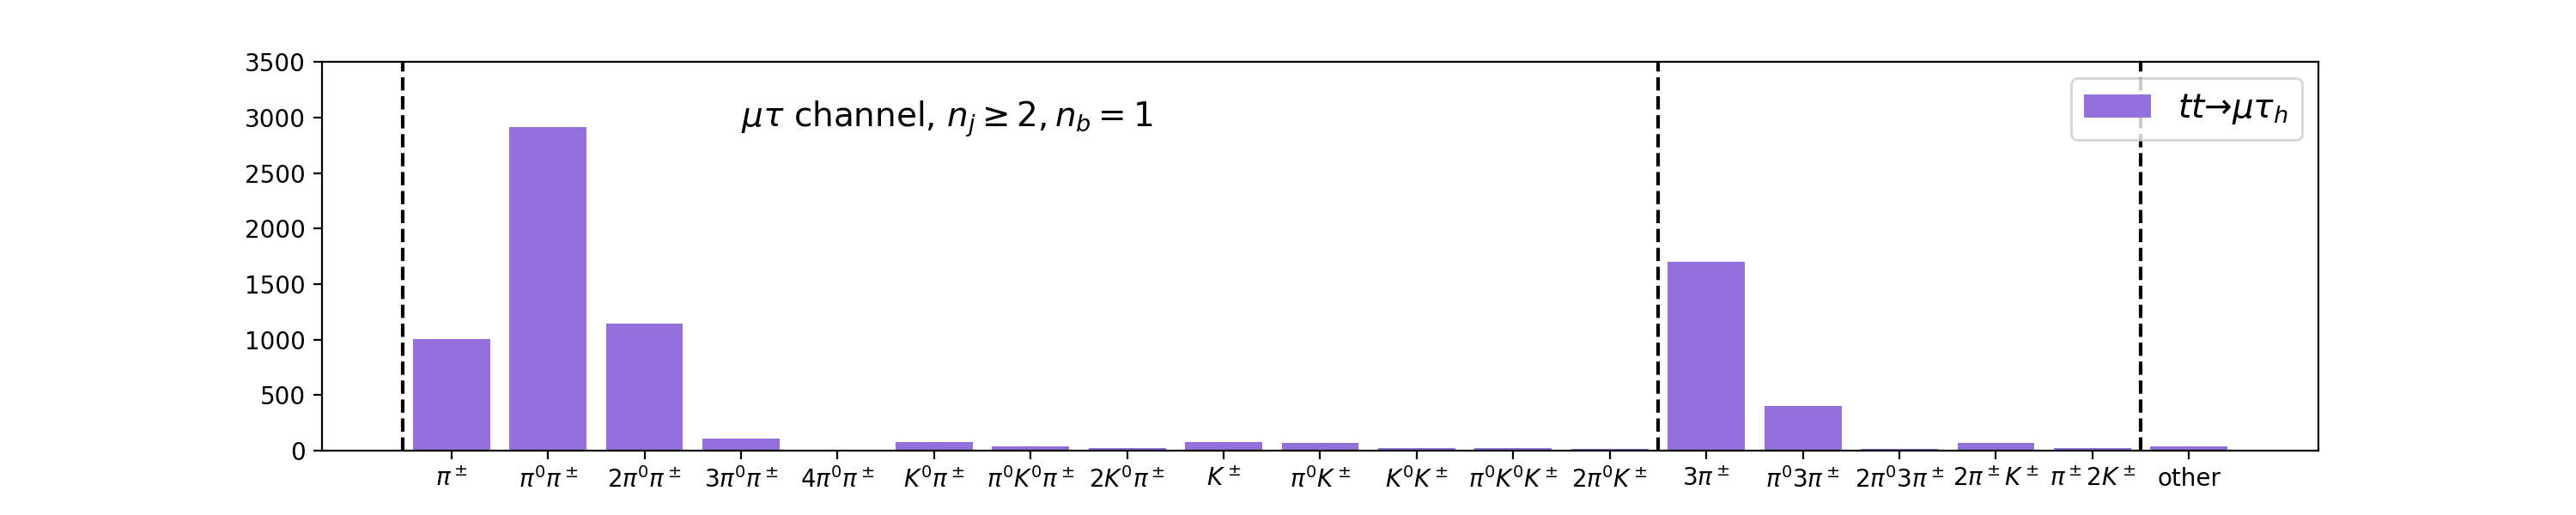
\includegraphics[width=0.99\textwidth]{chapters/Analysis/sectionCalibration/figures/tauBr/tauhDecay_mutau.png}
    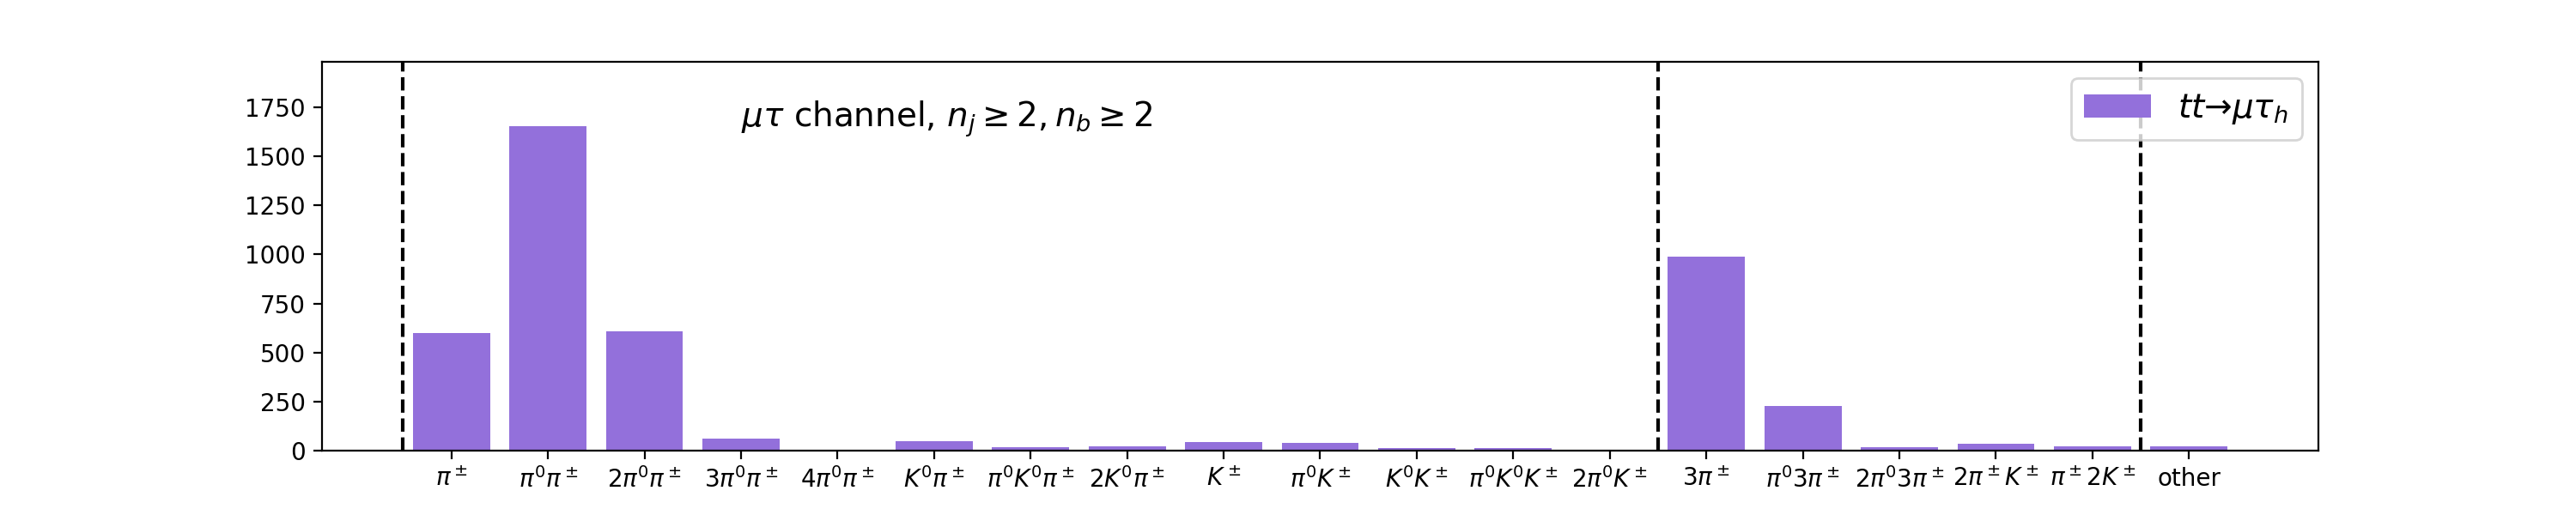
\includegraphics[width=0.99\textwidth]{chapters/Analysis/sectionCalibration/figures/tauBr/tauhDecay_mutau2.png}
    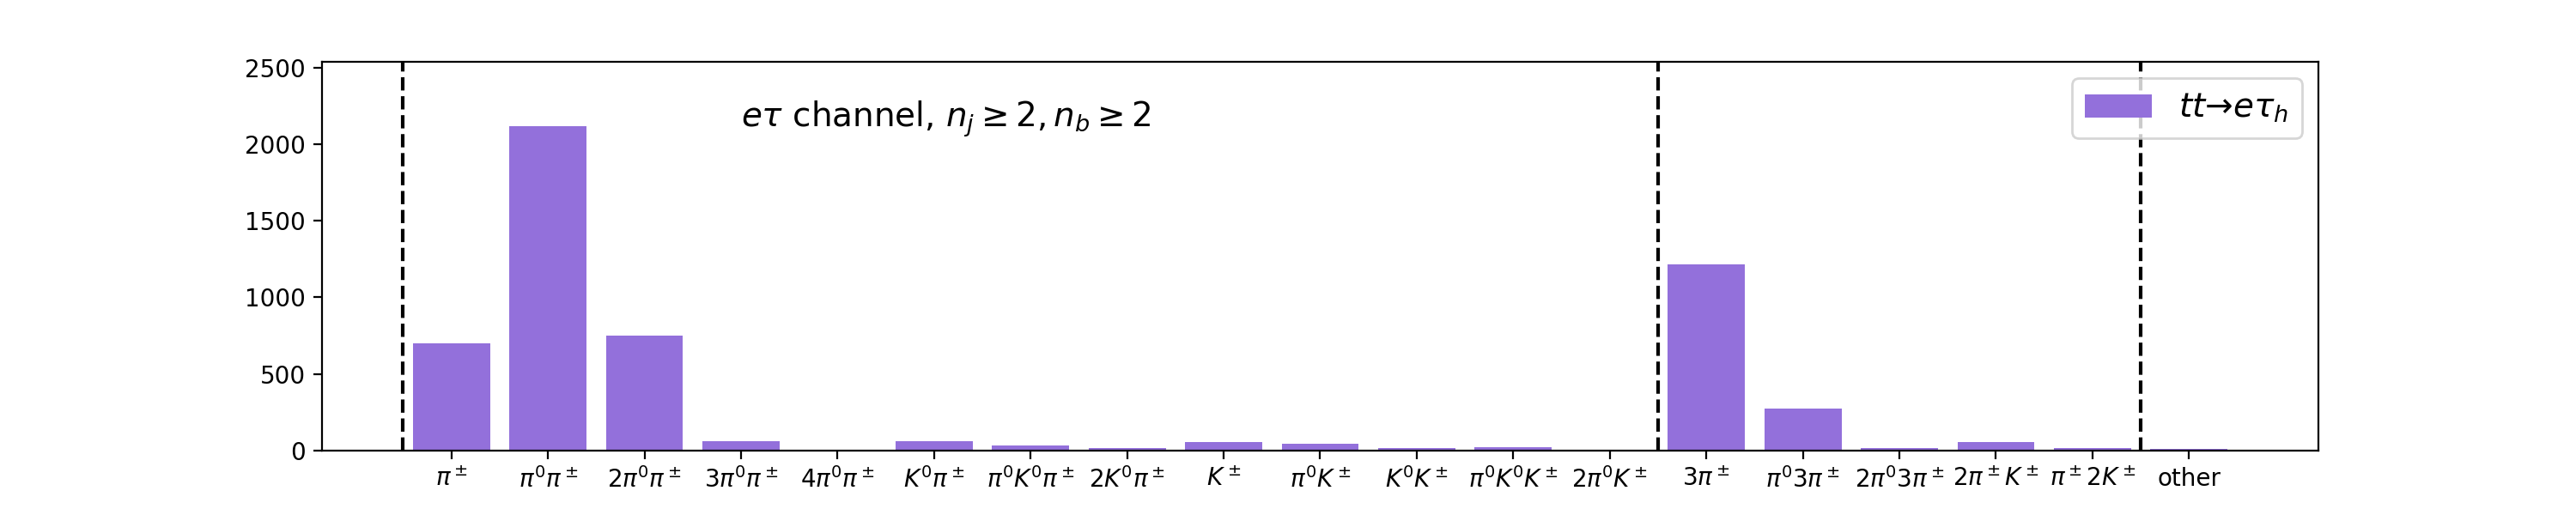
\includegraphics[width=0.99\textwidth]{chapters/Analysis/sectionCalibration/figures/tauBr/tauhDecay_etau.png}
    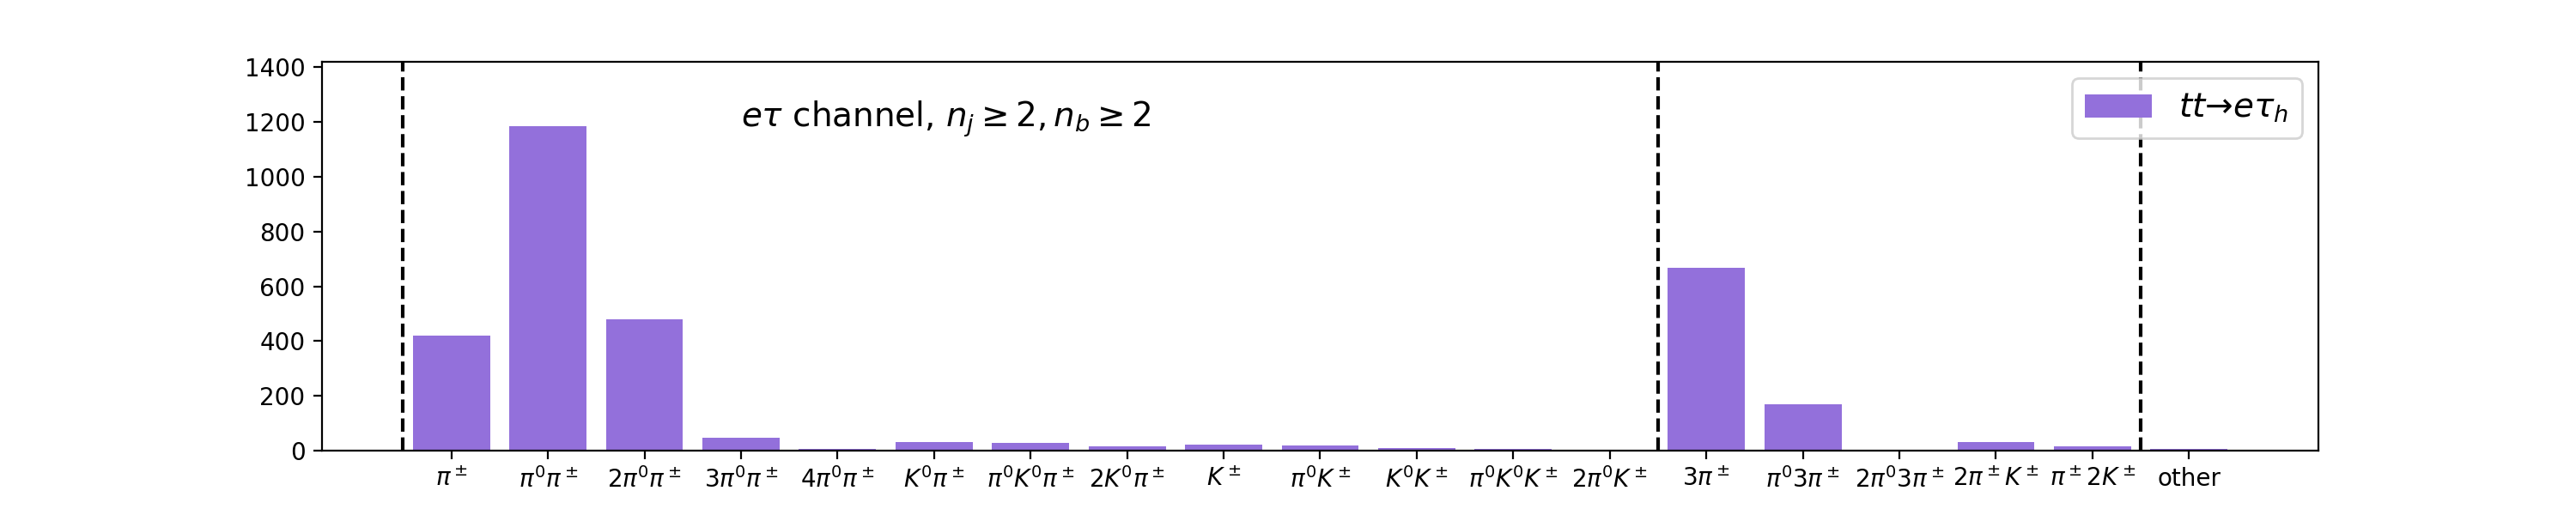
\includegraphics[width=0.99\textwidth]{chapters/Analysis/sectionCalibration/figures/tauBr/tauhDecay_etau2.png}
    \caption{The gen-level daughter mesons from hadronicly decaying taus in the $tt\to \mu \tau_h, e \tau_h$ events passing $\mu \tau$ and $e \tau$ selection.}
    \label{fig:appendix:reweightTauhBr:tauhBr}
\end{figure}


In MC events, the gen-level daughter mesons from hadronically decaying taus are saved.  The $\tau_h$'s daughter mesons in the $tt\to \mu \tau_h, e \tau_h$ events  passing $\mu \tau$ and $e \tau$ selection are shown in Fig~\ref{fig:appendix:reweightTauhBr:tauhBr} The leading contributions to the reconstructed $\tau_h$ are $\tau\to \pi^\pm+\pi^0 $, $\tau\to 3\pi^\pm$, $\tau\to \pi^\pm+2\pi^0$, $\tau\to \pi^\pm$, $\tau\to 3\pi^\pm + \pi^0$.  MC events with taus in those five decay modes are reweighted by 

\begin{equation}
  w = \frac{^{\rm PDG} B(\tau \to  \rm{hadrons}) }{^{\rm \PYTHIA} B( \tau \to \rm{hadrons} )}. 
\end{equation} 


\noindent The uncertainties of the weights are from the the PDG uncertainties.  The systematical uncertainty due to the uncertainties of $B(\tau \to  \rm{hadrons})$ reweighting can be estimated. The effect of the $B(\tau \to  \rm{hadrons})$  reweighting on the $B(W)$ result is small. The relative systematics from $B(\tau \to  \rm{hadrons})$ reweighting are about $0.003 - 0.146 \%$,  shown in table~ \ref{tab:syst_tauhReweighting}.



\begin{table}[p]
  \centering
  \caption{ Relative systematic uncertainty ($\%$) due to $B(\tau \to  \rm{hadrons})$ reweighting.}
  \setlength{\tabcolsep}{0.5 em}
  \renewcommand{\arraystretch}{2}
  \resizebox{\textwidth}{!}{
  \begin{tabular}{|l|ccc|ccc|ccc|ccc|ccc|}
    \hline
    Error Source & \multicolumn{3}{c|}{$\mu$-1b} & \multicolumn{3}{c|}{$\mu$-2b} & \multicolumn{3}{c|}{$e$-1b} & \multicolumn{3}{c|}{$e$-2b} \\
    \hline
                  & $B_e$ & $B_\mu$ & $B_\tau$ & $B_e$ & $B_\mu$ & $B_\tau$ & $B_e$ & $B_\mu$ & $B_\tau$ & $B_e$ & $B_\mu$ & $B_\tau$ \\
    \hline
    0.5$\%$ err of $Br_{\tau\to\pi^\pm}$       & 0.009 & 0.013 & 0.055 & 0.009 & 0.012 & 0.051 & 0.009 & 0.012 & 0.052 & 0.010 & 0.012 & 0.057 \\ 
    0.5$\%$ err of $Br_{\tau\to\pi^\pm\pi^0}$  & 0.025 & 0.033 & 0.141 & 0.026 & 0.033 & 0.147 & 0.024 & 0.032 & 0.146 & 0.025 & 0.032 & 0.146 \\ 
    0.2$\%$ err of $Br_{\tau\to\pi^\pm2\pi^0}$ & 0.003 & 0.004 & 0.017 & 0.003 & 0.004 & 0.015 & 0.003 & 0.004 & 0.017 & 0.003 & 0.004 & 0.019 \\ 
    0.6$\%$ err of $Br_{\tau\to3\pi^\pm}$      & 0.017 & 0.022 & 0.101 & 0.019 & 0.023 & 0.111 & 0.017 & 0.023 & 0.107 & 0.017 & 0.022 & 0.107 \\ 
    0.6$\%$ err of $Br_{\tau\to3\pi^\pm\pi^0}$ & 0.005 & 0.006 & 0.024 & 0.005 & 0.006 & 0.022 & 0.004 & 0.006 & 0.022 & 0.005 & 0.006 & 0.025 \\ 
    \hline
  \end{tabular}}
  \label{tab:syst_tauhReweighting}
\end{table}
\FloatBarrier
